\documentclass[UTF8]{ctexart}

%----------- 版式与字体 ----------------
\usepackage{geometry}
\geometry{a4paper,margin=2.5cm}
\setlength{\parindent}{2em}
\setlength{\parskip}{0.5em}
\renewcommand{\baselinestretch}{1.3}

%----------- 列表与颜色 ----------------
\usepackage[shortlabels]{enumitem}
\setlist[enumerate]{label=\arabic*.}
\usepackage{xcolor}
\usepackage{titlesec}

%----------- 数学宏包 ------------------
\usepackage{amsmath}
\usepackage{amsfonts}
\usepackage{amssymb}

% 添加必要的宏包
\usepackage{graphicx} % 支持插入图片
\usepackage{subcaption} % 支持子图
\usepackage{siunitx}
\usepackage{listings}
\lstset{language=Python, basicstyle=\ttfamily\footnotesize, showstringspaces=false, tabsize=4}


%----------- 题注样式(节标题) ---------
\titleformat{\section}
  {\zihao{4}\bfseries}{\chinese{section}、}{0.5em}{}
\titleformat{\subsection}
  {\zihao{5}\bfseries}{\arabic{section}.\arabic{subsection}}{0.5em}{}

%----------- 正文开始 ------------------
\begin{document}

\begin{center}
  {\zihao{3}\bfseries 人工智能实验报告}\\[1ex]
  {\zihao{4} 实验二\quad 传统机器学习方法}
\end{center}

% ----------- 信息栏 -------------------
\renewcommand{\arraystretch}{1.6}
\begin{tabular}{p{5cm}p{5.5cm}p{3cm}p{5.5cm}}
  学院:计算机与通信工程 & 专业:计算机科学与技术 & 班级:计221\\
  姓名:乔彦博 & 学号:U202242223 & 日期:2025.5.9\\
\end{tabular}

% ----------- 一、实验目标 --------------
\section*{实验目标}
\begin{enumerate}
  \item 掌握传统机器学习的基本流程和方法,包括熟悉数据预处理、特征工程、模型训练与评估展示等完整流程;理解传统机器学习算法的核心原理(如分类、回归、聚类等)。
  
  \item 通过监督学习和无监督学习实验,理解不同算法的应用场景和效果评估。监督学习例如分类算法(如KNN、决策树、SVM等),对比分类性能;无监督学习例如聚类算法(如K-Means、层次聚类等),分析聚类效果。
  
  \item 通过可视化展示,深入理解数据和模型,包括:
    \begin{itemize}
      \item 数据可视化:使用散点图、箱线图、平行坐标图等展示数据集特征分布和类别差异
      \item 模型可视化:对监督学习模型,绘制决策边界(如决策树、SVM)或特征重要性(如随机森林);对无监督学习模型,展示聚类结果(如K-Means的聚类中心、聚类分布)等
      \item 效果可视化:使用混淆矩阵热力图、ROC曲线等展示分类模型的性能;使用肘部法则图、轮廓系数图等展示聚类模型的效果
    \end{itemize}
\end{enumerate}

% ----------- 二、实验内容 --------------
\section*{实验内容}
\subsection*{1. 任务分析}
本实验主要针对传统机器学习方法的应用与实践,包含两大核心任务:

\begin{enumerate}
  \item \textbf{监督学习任务}:选择合适的分类数据集,实现并对比多种分类算法(如KNN、决策树、SVM等)的性能。需要完成数据预处理、特征选择、模型训练、参数调优及结果评估等步骤。通过混淆矩阵、精确率、召回率、F1分数等指标对各算法效果进行全面评估。
  
  \item \textbf{无监督学习任务}:选择适合聚类的数据集,实现K-Means、层次聚类等算法,并通过轮廓系数、肘部法则等方法评估聚类效果。重点分析不同聚类算法的特点及适用场景。
\end{enumerate}

两项任务均要求通过可视化技术增强对数据特征和算法性能的直观理解,包括数据分布可视化、决策边界可视化和评估指标可视化等。

\subsection*{2. 实现工具}
本实验采用以下工具和技术栈:

\begin{itemize}
  \item \textbf{编程语言}:Python 3.11.12,采用3.11最新版本,安全性更好
  
  \item \textbf{数据处理库}:
    \begin{itemize}
      \item NumPy:用于高效的数值计算和数组操作
      \item Pandas:用于数据加载、清洗和预处理
    \end{itemize}
  
  \item \textbf{机器学习库}:
    \begin{itemize}
      \item Scikit-learn:提供各种监督学习和无监督学习算法实现
      \item SciPy:用于科学计算的高级函数
    \end{itemize}
  
  \item \textbf{可视化工具}:
    \begin{itemize}
      \item Matplotlib:基础绘图库,用于生成各类统计图表
      \item Seaborn:基于Matplotlib的统计数据可视化库,用于生成更美观的图表
      \item Plotly:交互式可视化库(可选)
    \end{itemize}
    
  \item \textbf{开发环境}:Jupyter Notebook,便于代码与结果展示的交互式环境
\end{itemize}

\subsection*{3. 实现方案}
本实验的整体实施方案如下:

\begin{enumerate}
  \item \textbf{数据准备阶段}
    \begin{itemize}
      \item 监督学习:选择UCI机器学习仓库中的Iris数据集和Wine数据集
      \item 无监督学习:使用相同数据集但不使用标签信息
      \item 数据分析:统计特征、相关性分析、缺失值处理
      \item 数据可视化:绘制特征分布图、散点矩阵、箱线图等
    \end{itemize}
  
  \item \textbf{监督学习实验}
    \begin{itemize}
      \item 数据预处理:特征标准化、训练集与测试集划分(比例7:3)
      \item 模型实现:KNN(K=1,3,5,7)、决策树、随机森林、SVM(线性和RBF核)
      \item 模型评估:交叉验证、网格搜索最优参数
      \item 结果分析:计算准确率、精确率、召回率,绘制混淆矩阵、ROC曲线
      \item 可视化:绘制决策边界、特征重要性图表
    \end{itemize}
  
  \item \textbf{无监督学习实验}
    \begin{itemize}
      \item 数据预处理:特征标准化、降维(PCA)用于可视化
      \item 模型实现:K-Means(不同K值)、层次聚类(不同距离度量和链接方式)
      \item 最优聚类数确定:绘制肘部法则图、轮廓系数分析
      \item 聚类结果评估:与真实标签对比(如有)、聚类内/间距离计算
      \item 可视化:聚类结果散点图、聚类中心、层次聚类树状图
    \end{itemize}
  
  \item \textbf{结果分析与比较}
    \begin{itemize}
      \item 不同监督学习算法性能对比分析
      \item 不同无监督学习算法聚类效果对比
      \item 算法优缺点总结与适用场景分析
    \end{itemize}
\end{enumerate}

\subsection*{4. 实现内容}

\paragraph{4.1 监督学习模块(\texttt{task1.py})}
\begin{enumerate}[label=\arabic*)]
    \item \textbf{数据载入与缺失值注入}\\
          读取原始 \emph{Iris} 数据集后,以随机比例 \(\text{ratio}=0.1\) 将四个特征列注入缺失值,用于验证不同缺失值处理策略的鲁棒性。
    \item \textbf{缺失值处理策略}\\
          采用 \textit{drop}、\textit{mean}、\textit{median} 与 \textit{knn} 四种策略,对训练/测试集分别处理并保持标签一致。
    \item \textbf{特征缩放}\\
          填补或删除后使用 \texttt{StandardScaler} 归一化。
    \item \textbf{模型训练与评估}\\
          在四种策略下分别训练 \textbf{LogReg}、\textbf{Decision Tree}、\textbf{SVM (RBF)} 与 \textbf{KNN};记录 \emph{Accuracy} 与 \emph{Weighted \(F_1\)},并保存混淆矩阵。
\end{enumerate}

%----------------- 总体性能柱状图 -----------------
\begin{figure}[htbp]
    \centering
    \subfloat[Accuracy]{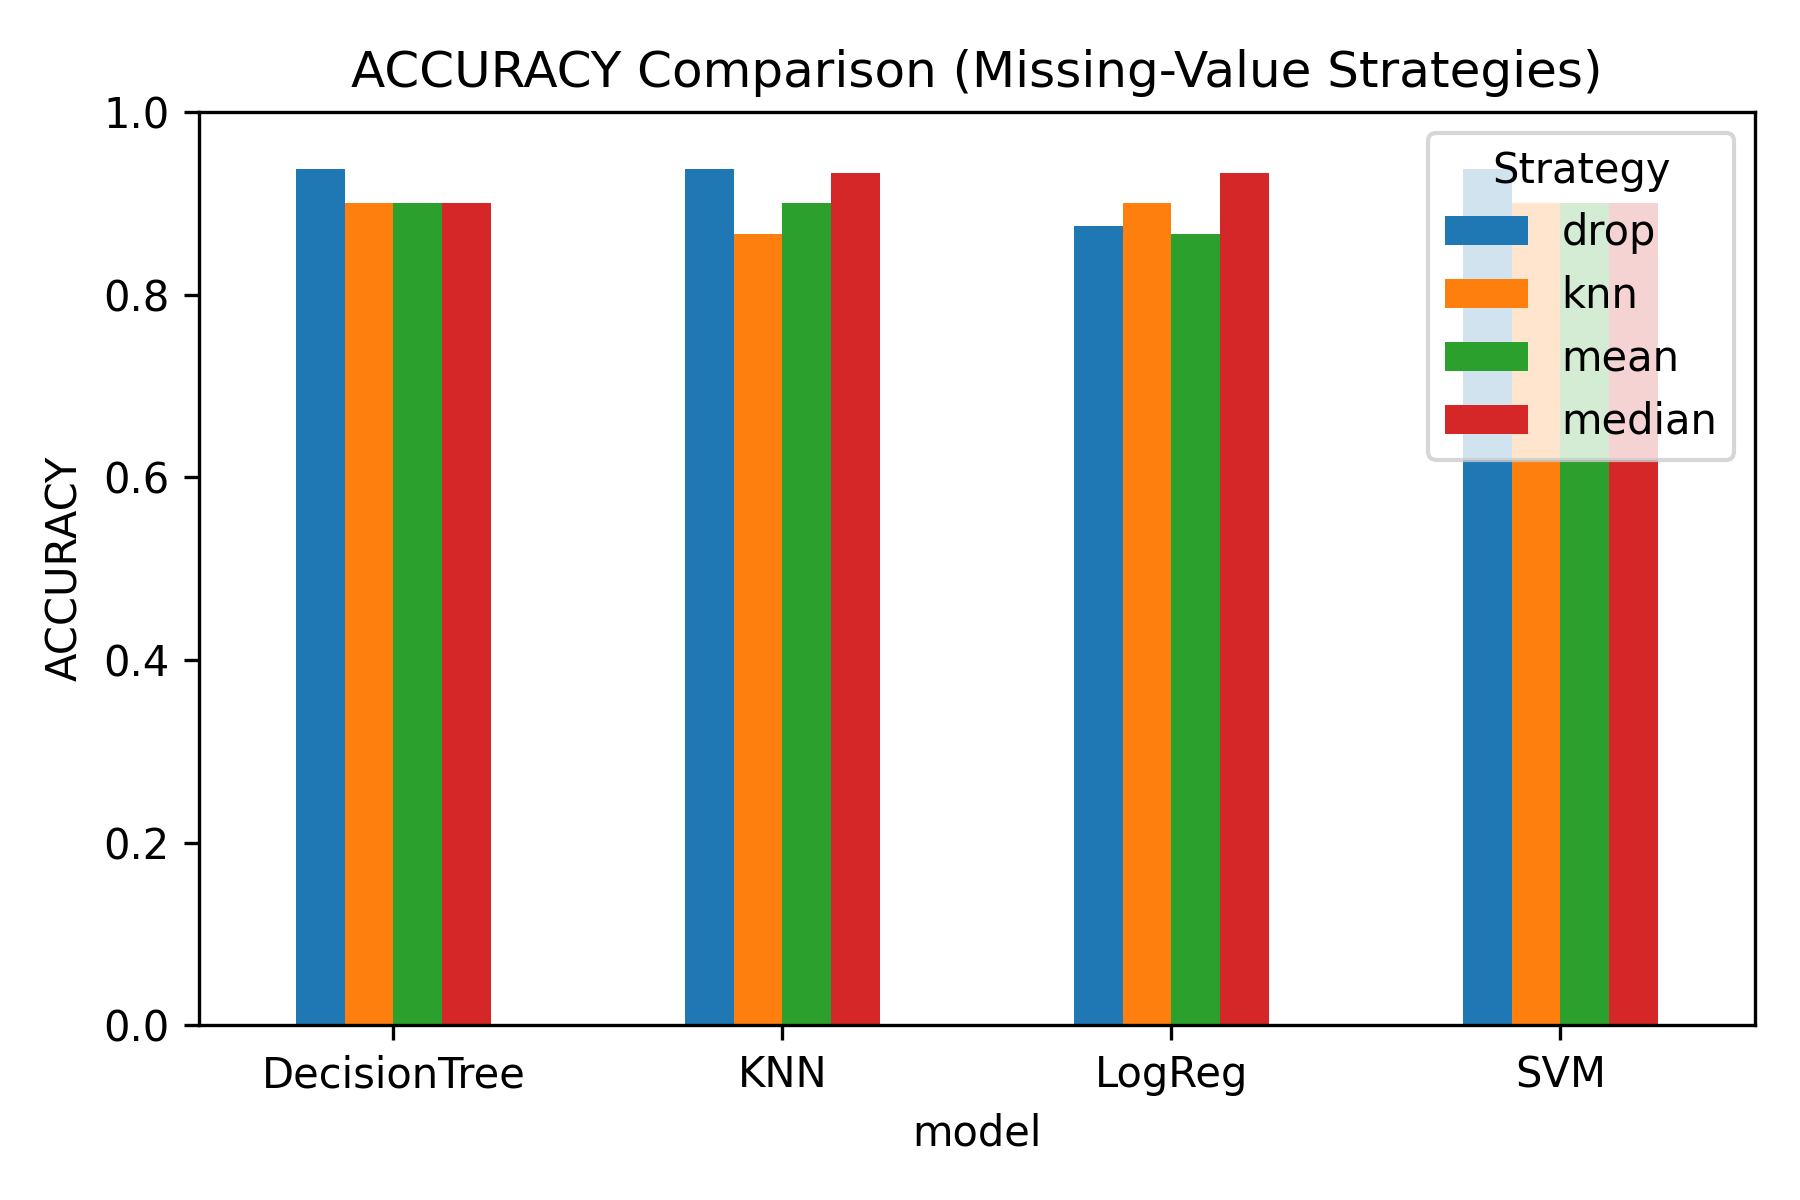
\includegraphics[width=0.45\linewidth]{figures/accuracy_comparison.png}}
    \hfill
    \subfloat[Weighted \(F_1\)]{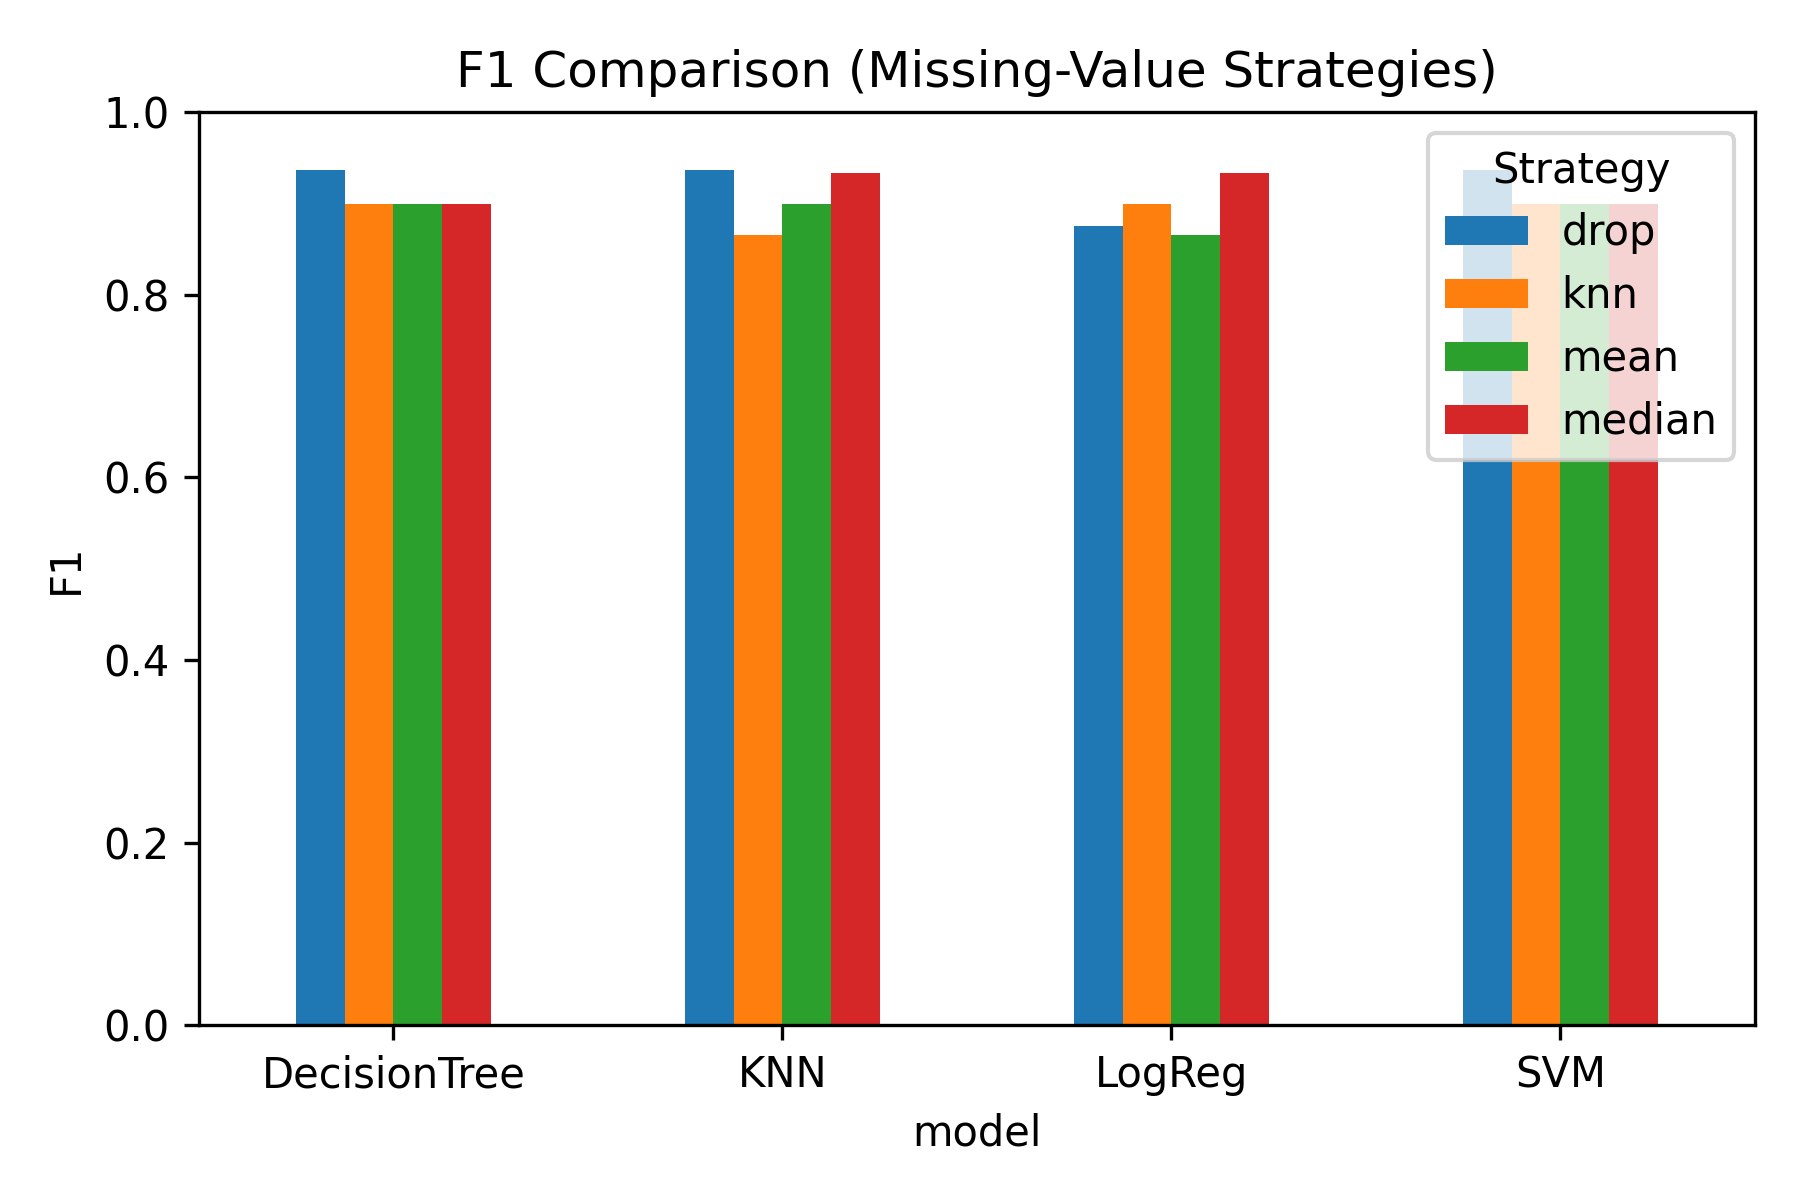
\includegraphics[width=0.45\linewidth]{figures/f1_comparison.png}}
    \caption{不同缺失值处理策略下四类模型的总体性能比较}
    \label{fig:acc_f1_bar}
\end{figure}

%----------------- 混淆矩阵 4×4 -----------------
\begin{figure}[htbp]
    \centering
    % --- drop ---
    \subfloat[drop--DecisionTree]{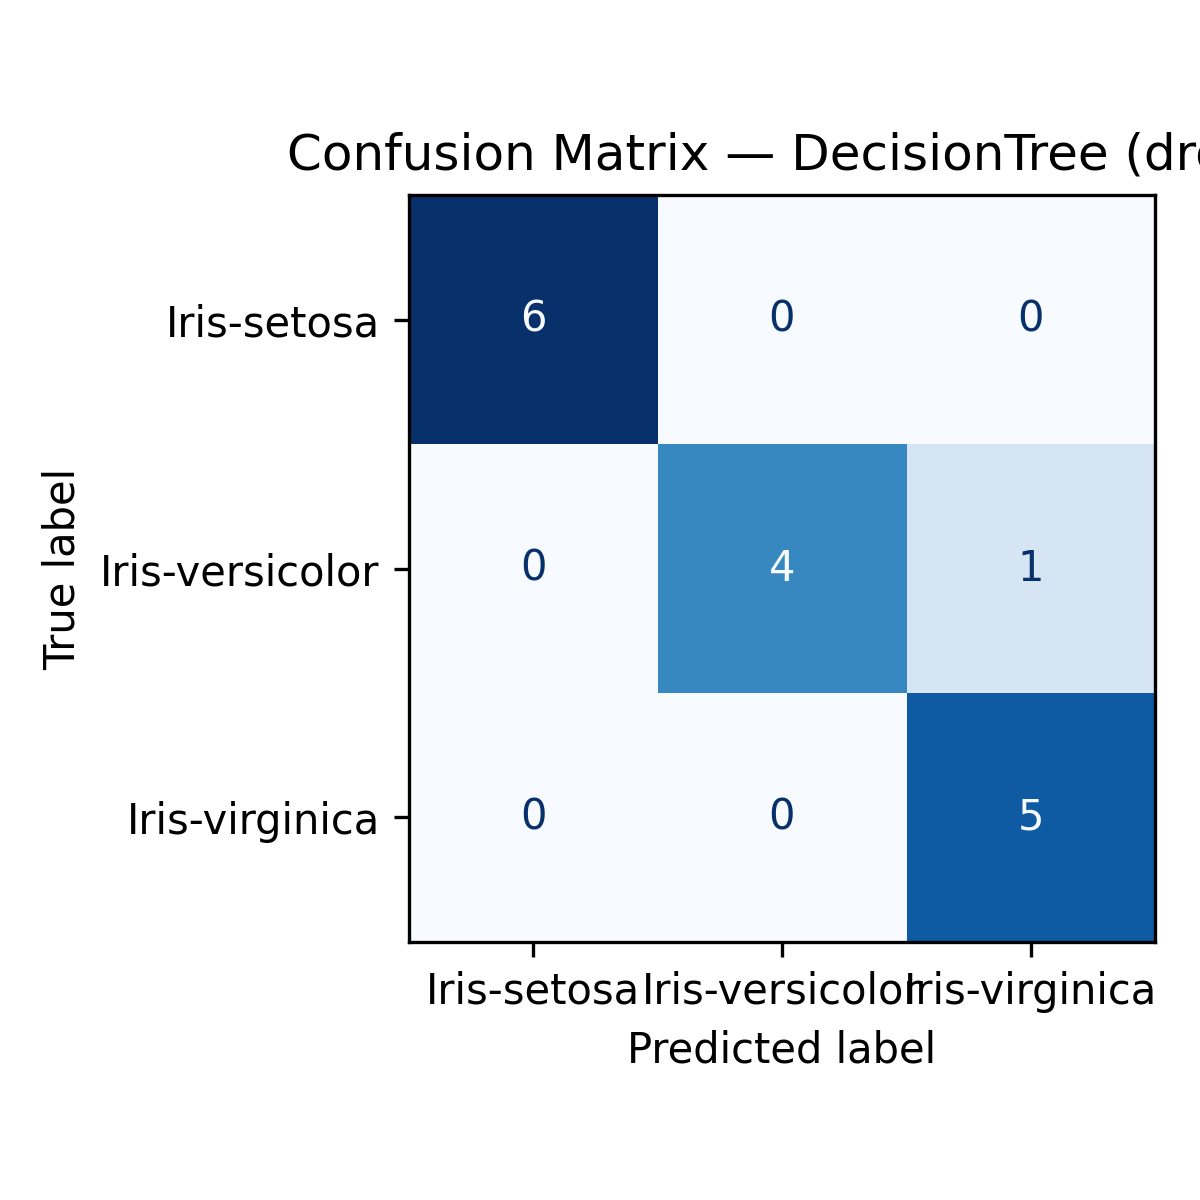
\includegraphics[width=0.22\linewidth]{figures/confmat_drop_DecisionTree.png}}
    \subfloat[drop--LogReg]{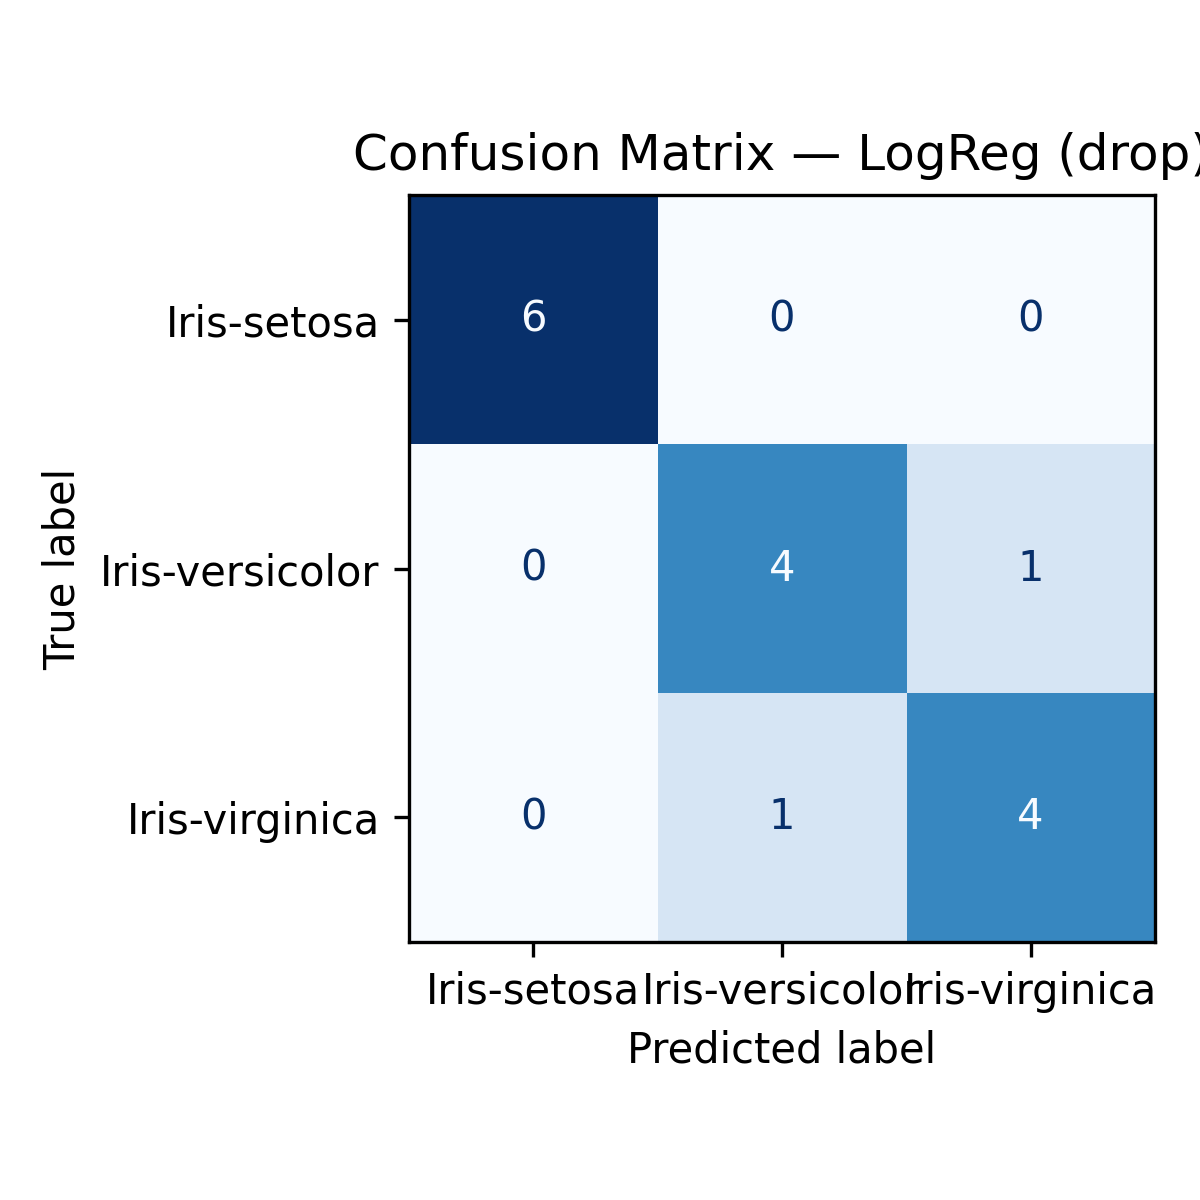
\includegraphics[width=0.22\linewidth]{figures/confmat_drop_LogReg.png}}
    \subfloat[drop--SVM]{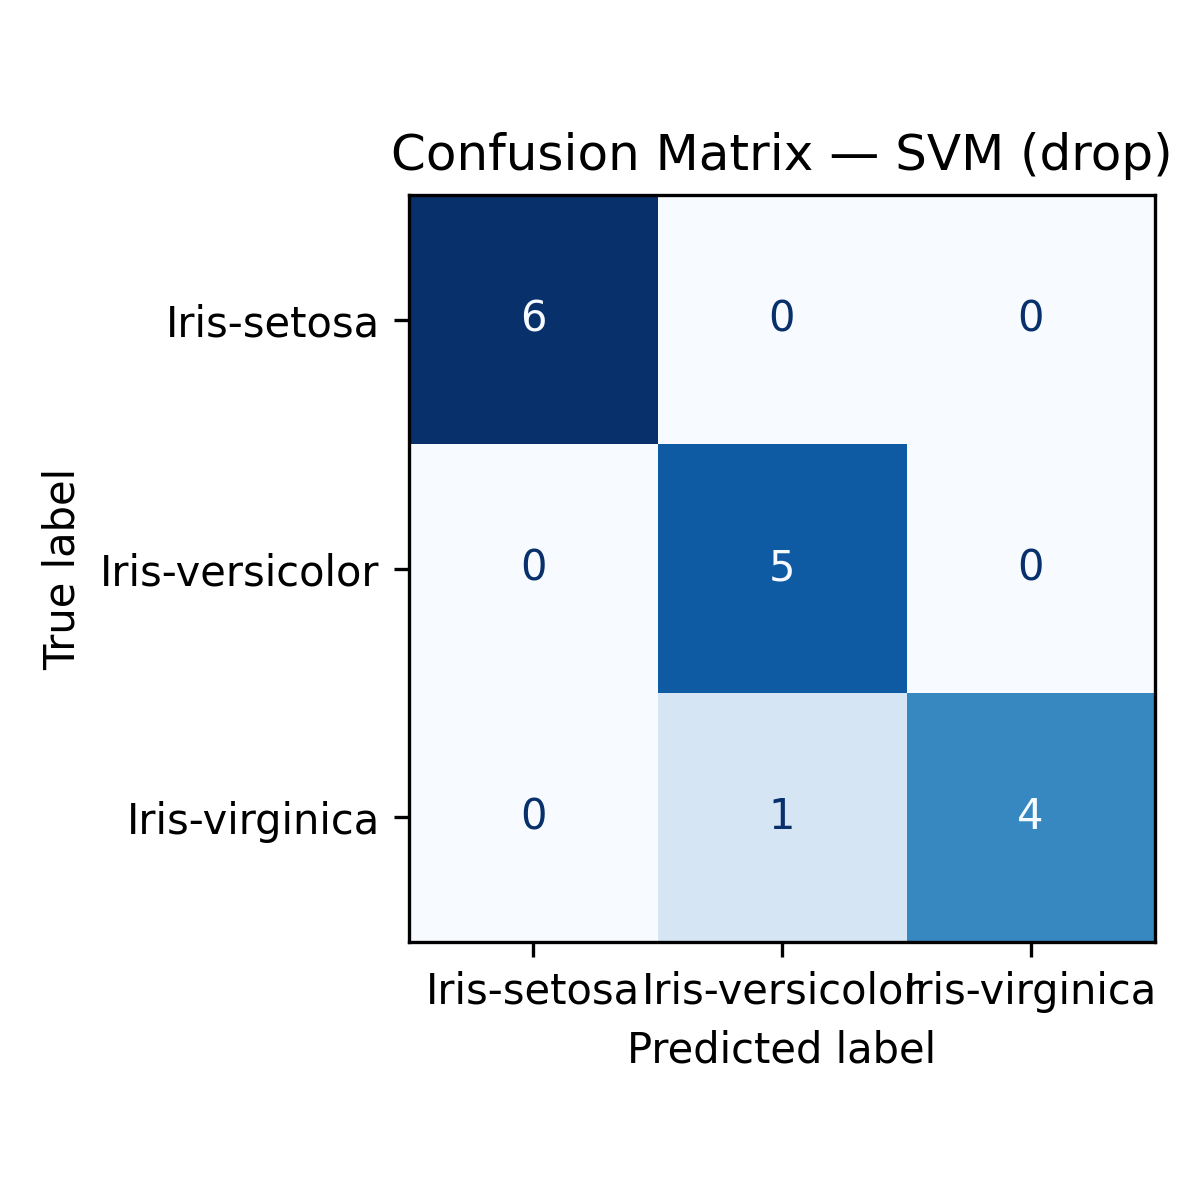
\includegraphics[width=0.22\linewidth]{figures/confmat_drop_SVM.png}}
    \subfloat[drop--KNN]{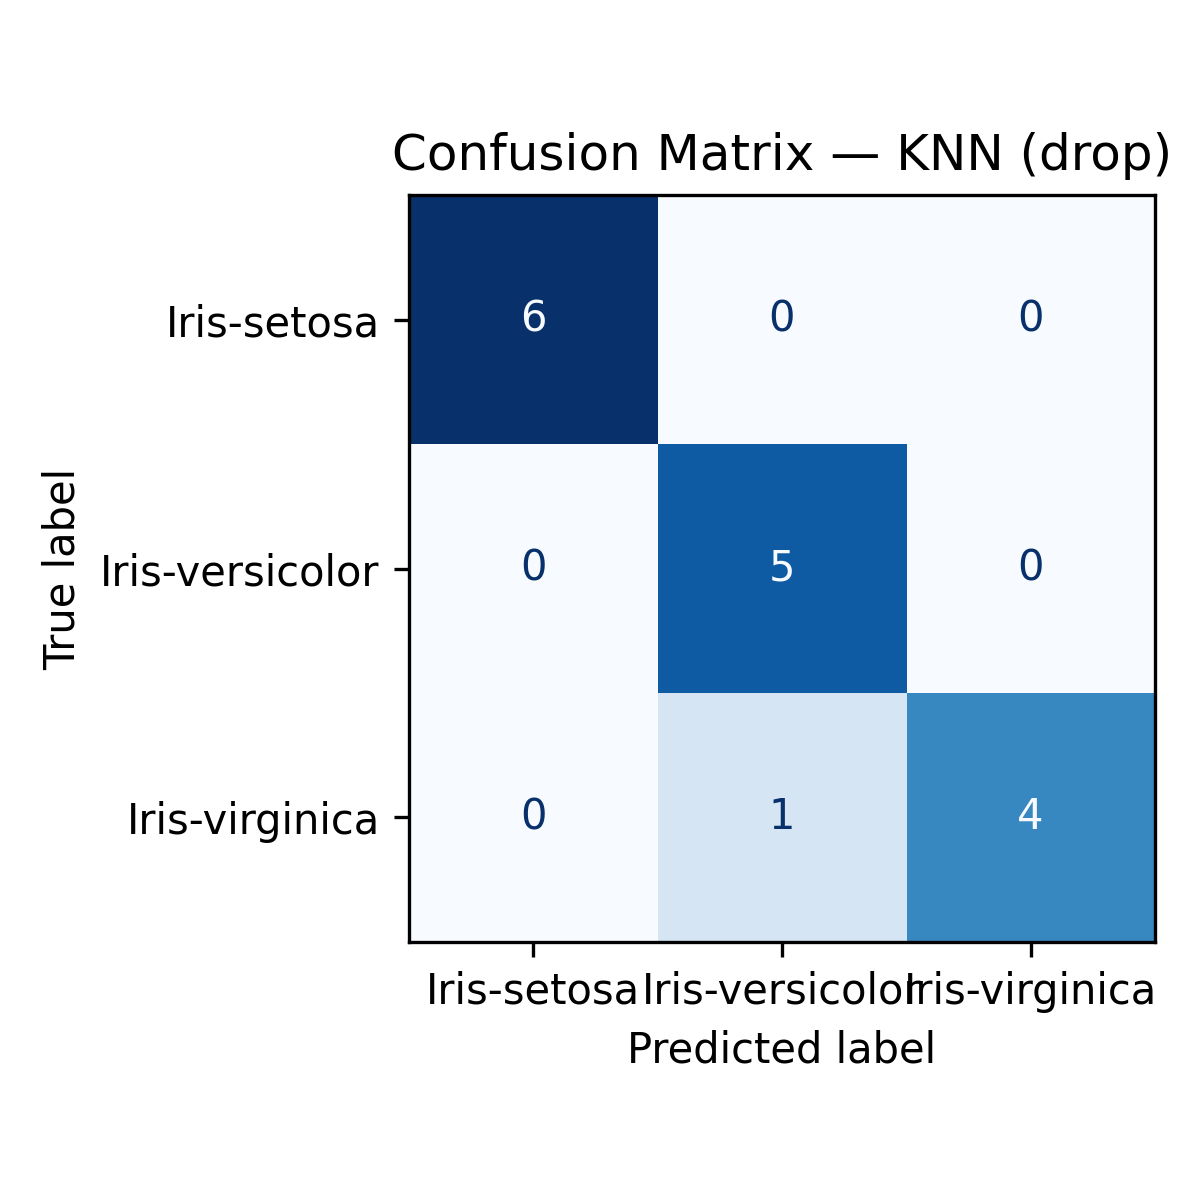
\includegraphics[width=0.22\linewidth]{figures/confmat_drop_KNN.png}}\\[0.4em]
    % --- mean ---
    \subfloat[mean--DecisionTree]{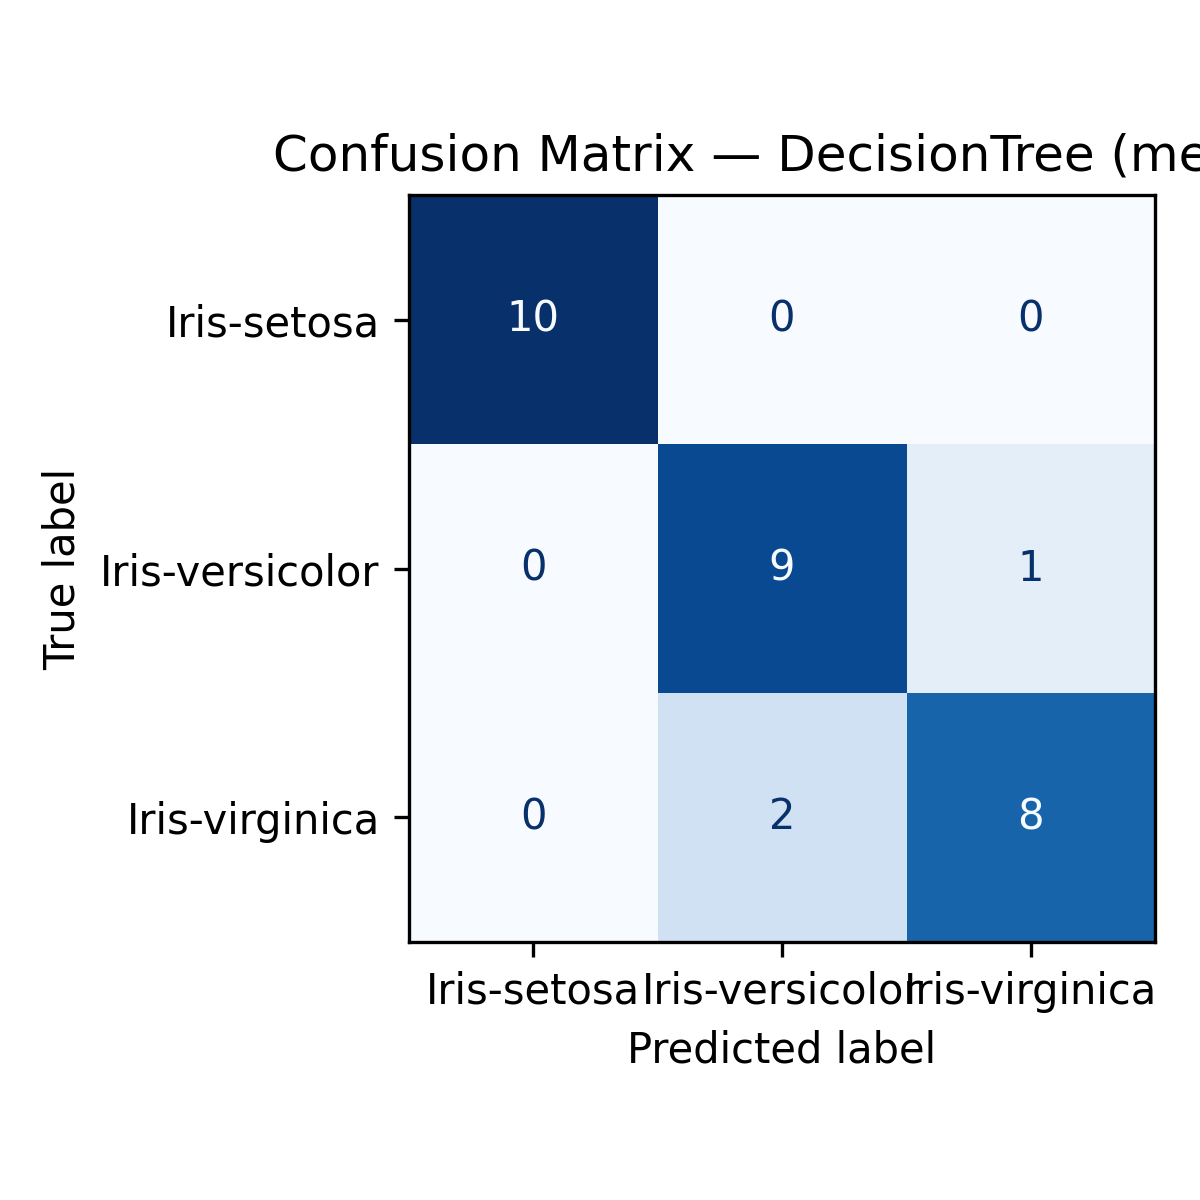
\includegraphics[width=0.22\linewidth]{figures/confmat_mean_DecisionTree.png}}
    \subfloat[mean--LogReg]{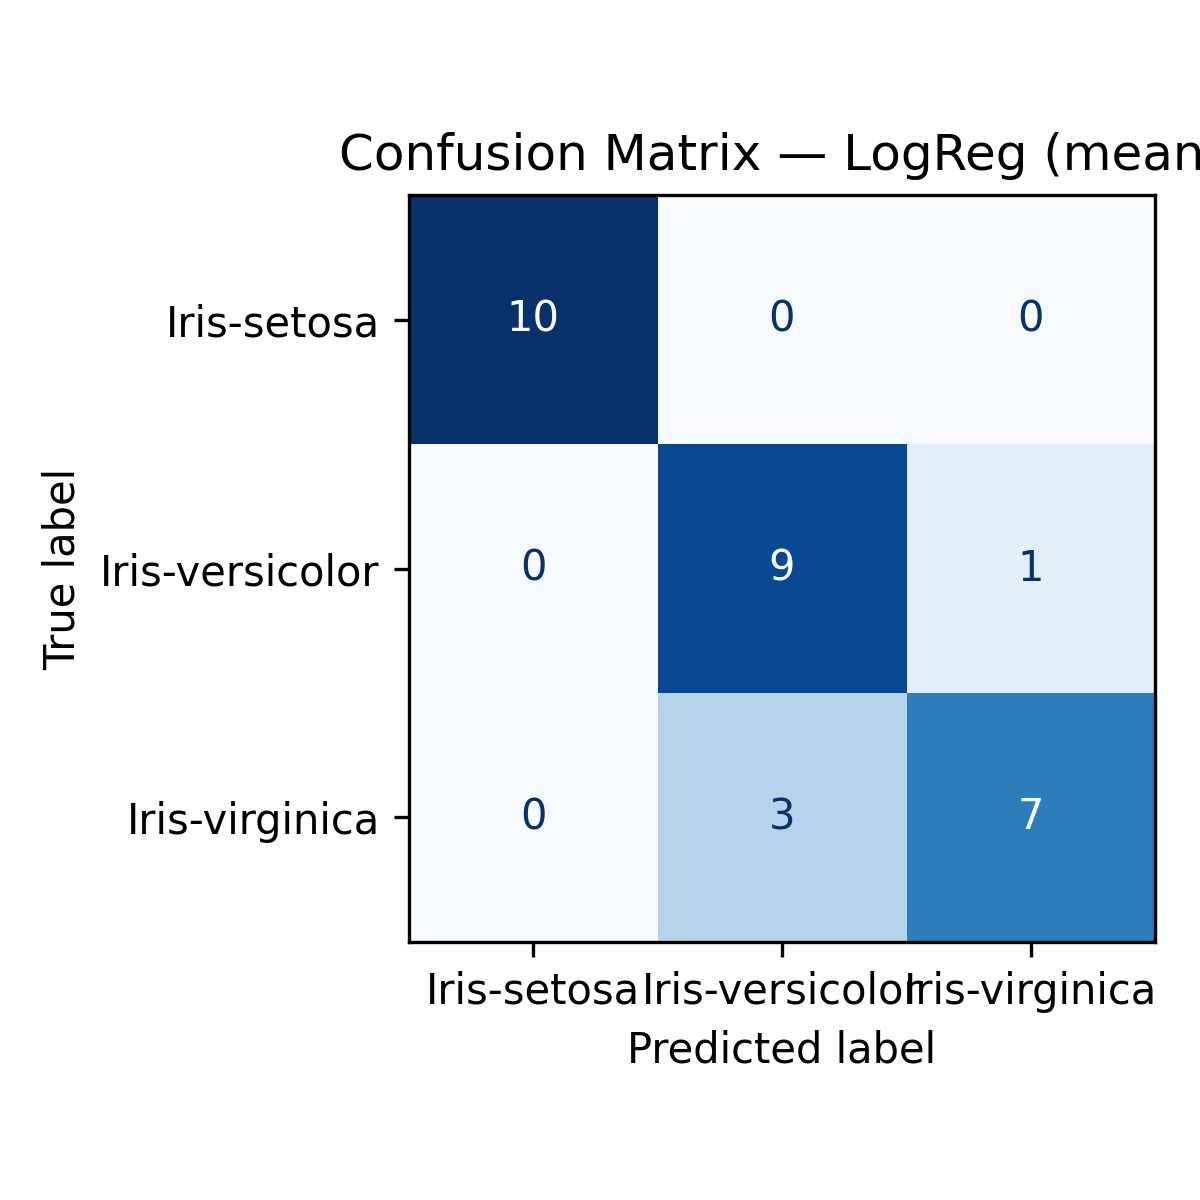
\includegraphics[width=0.22\linewidth]{figures/confmat_mean_LogReg.png}}
    \subfloat[mean--SVM]{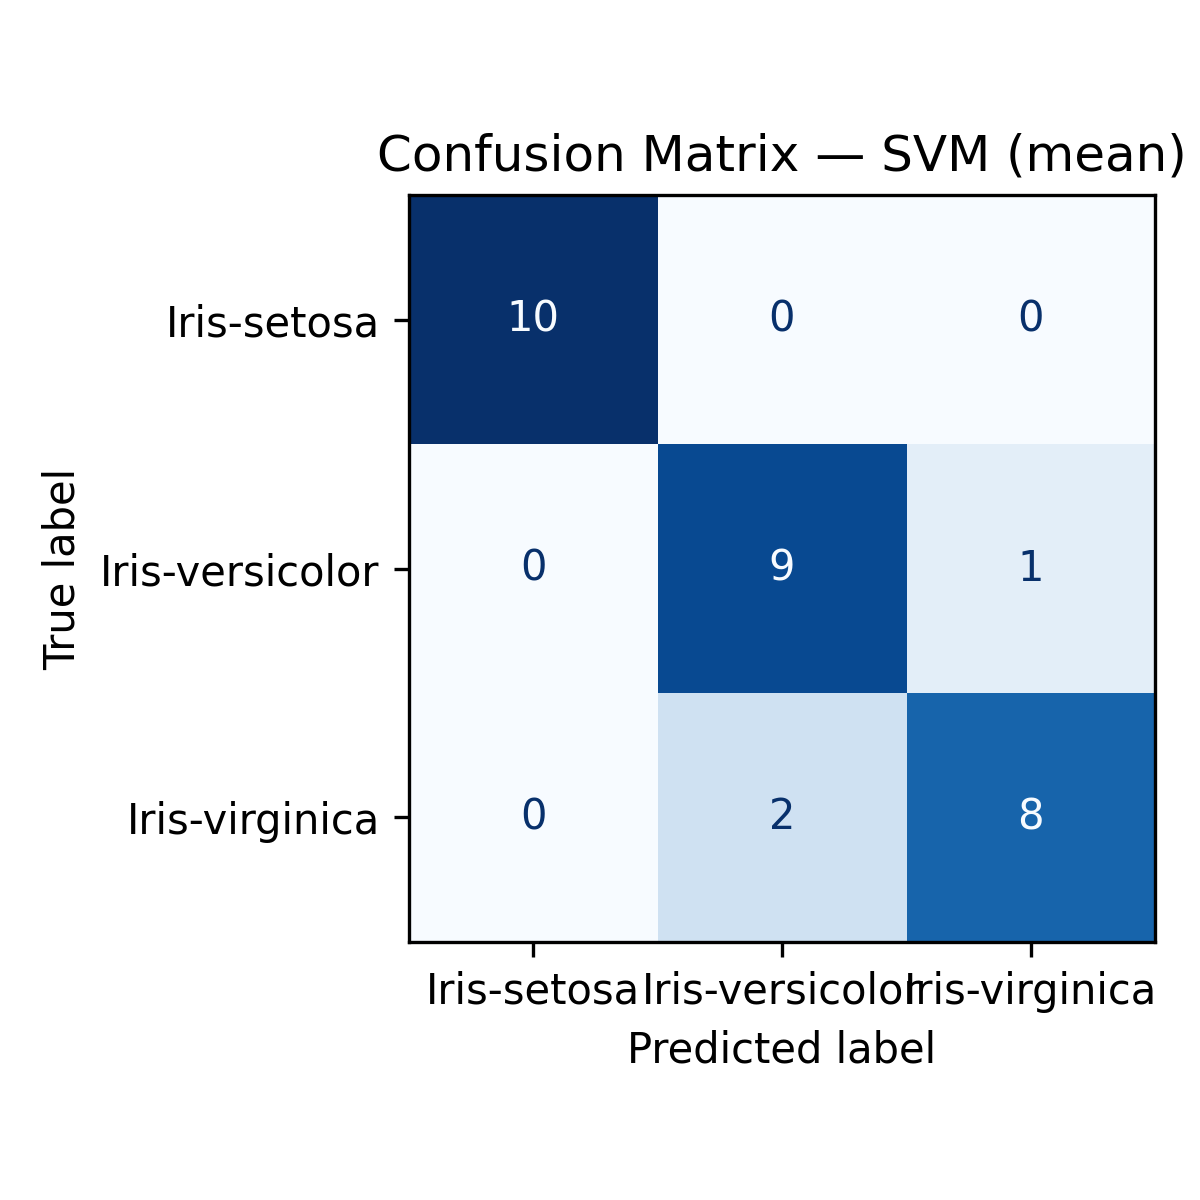
\includegraphics[width=0.22\linewidth]{figures/confmat_mean_SVM.png}}
    \subfloat[mean--KNN]{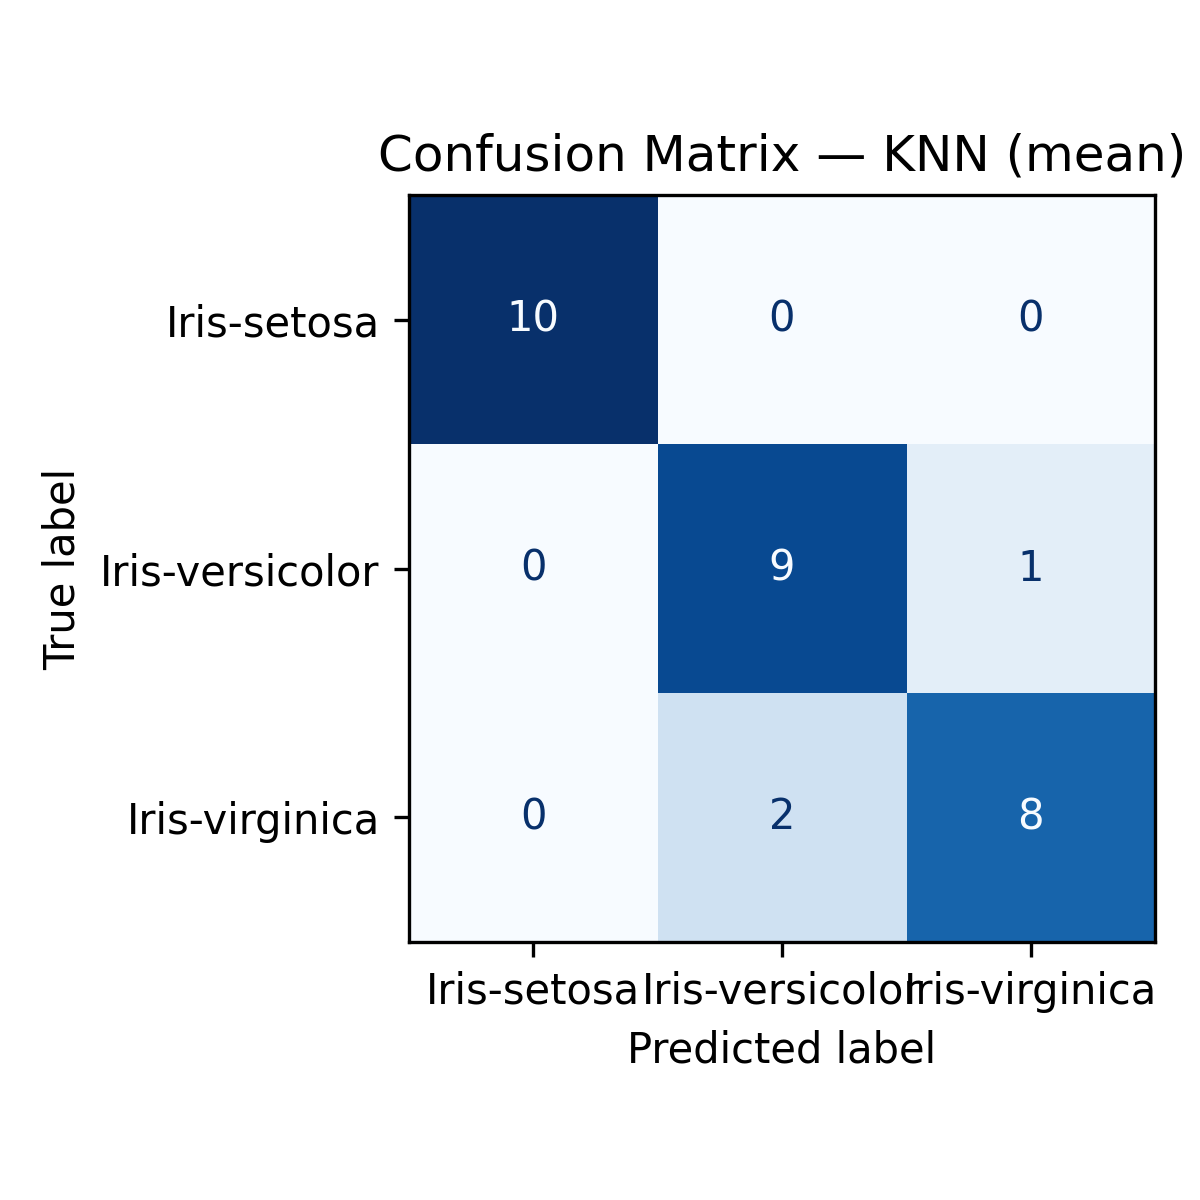
\includegraphics[width=0.22\linewidth]{figures/confmat_mean_KNN.png}}\\[0.4em]
    % --- median ---
    \subfloat[median--DecisionTree]{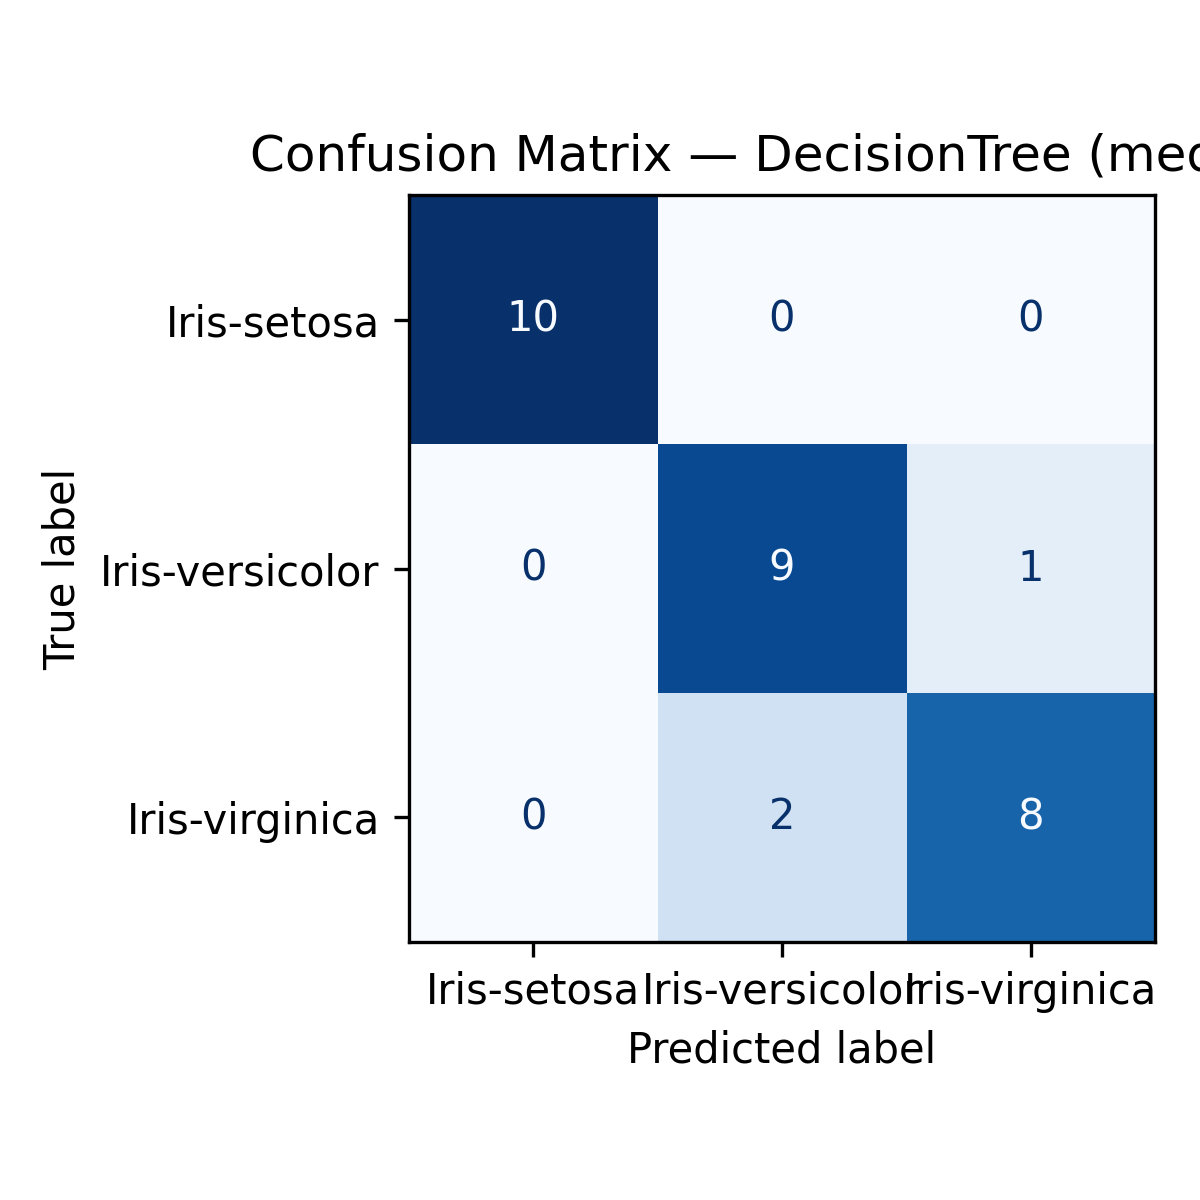
\includegraphics[width=0.22\linewidth]{figures/confmat_median_DecisionTree.png}}
    \subfloat[median--LogReg]{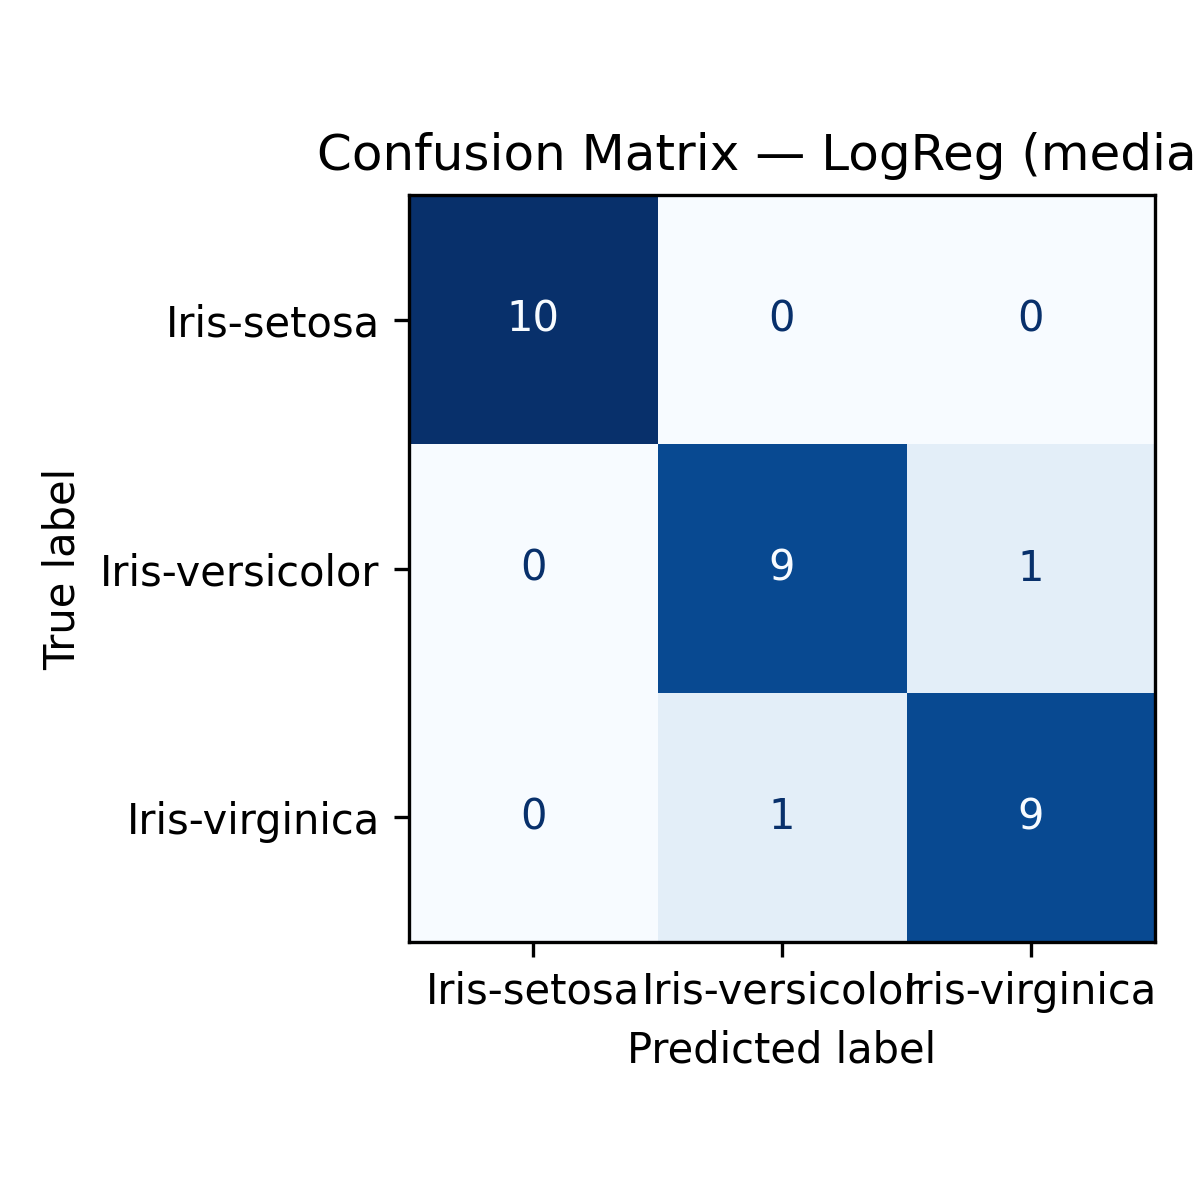
\includegraphics[width=0.22\linewidth]{figures/confmat_median_LogReg.png}}
    \subfloat[median--SVM]{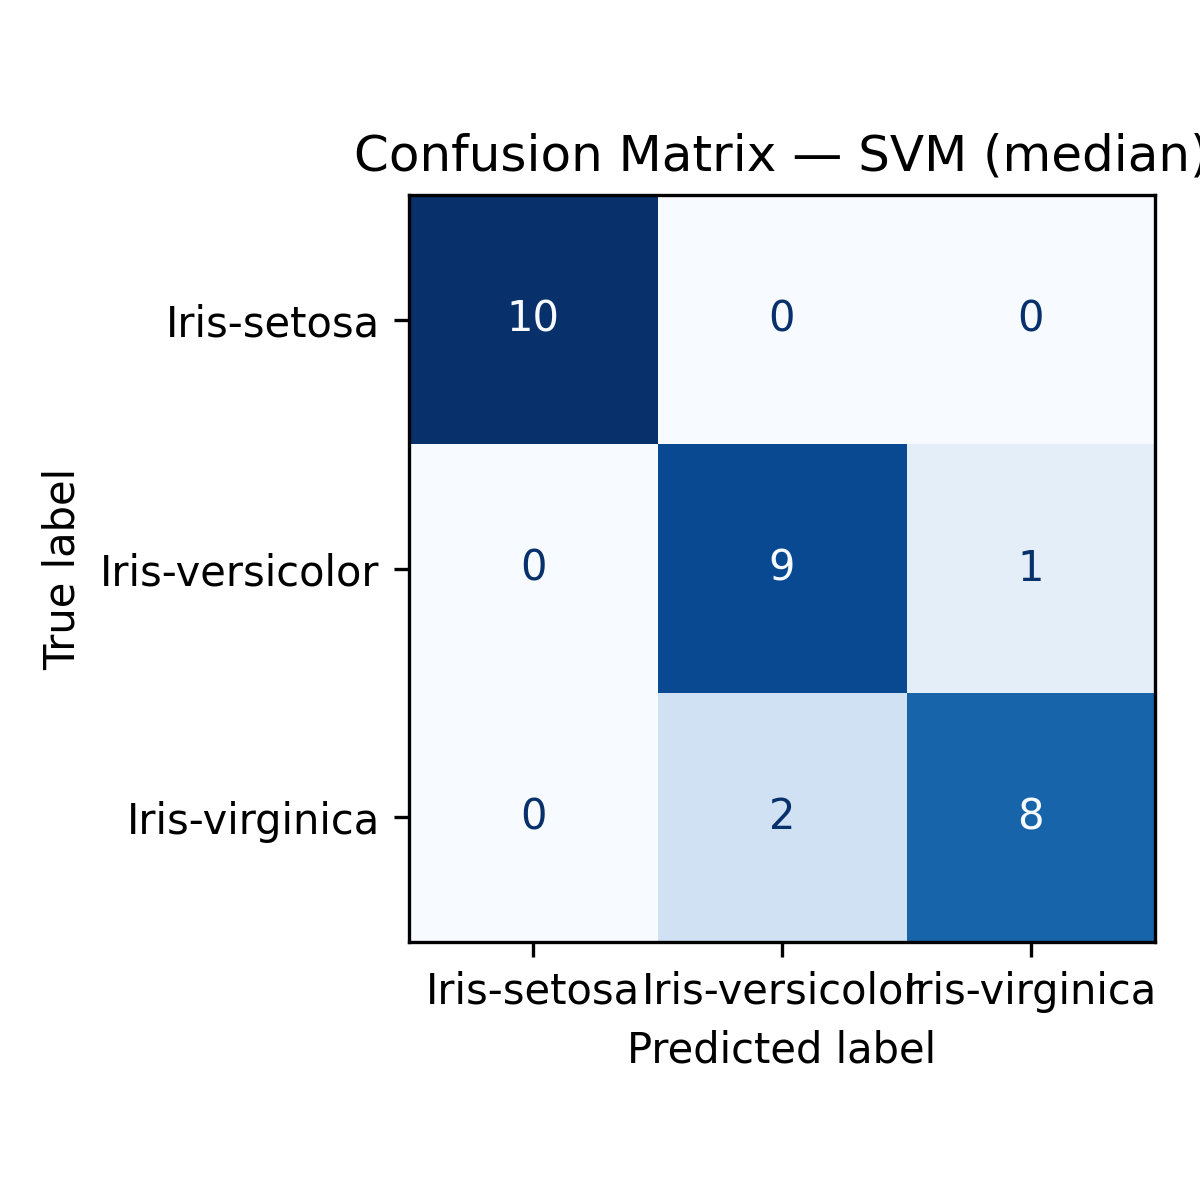
\includegraphics[width=0.22\linewidth]{figures/confmat_median_SVM.png}}
    \subfloat[median--KNN]{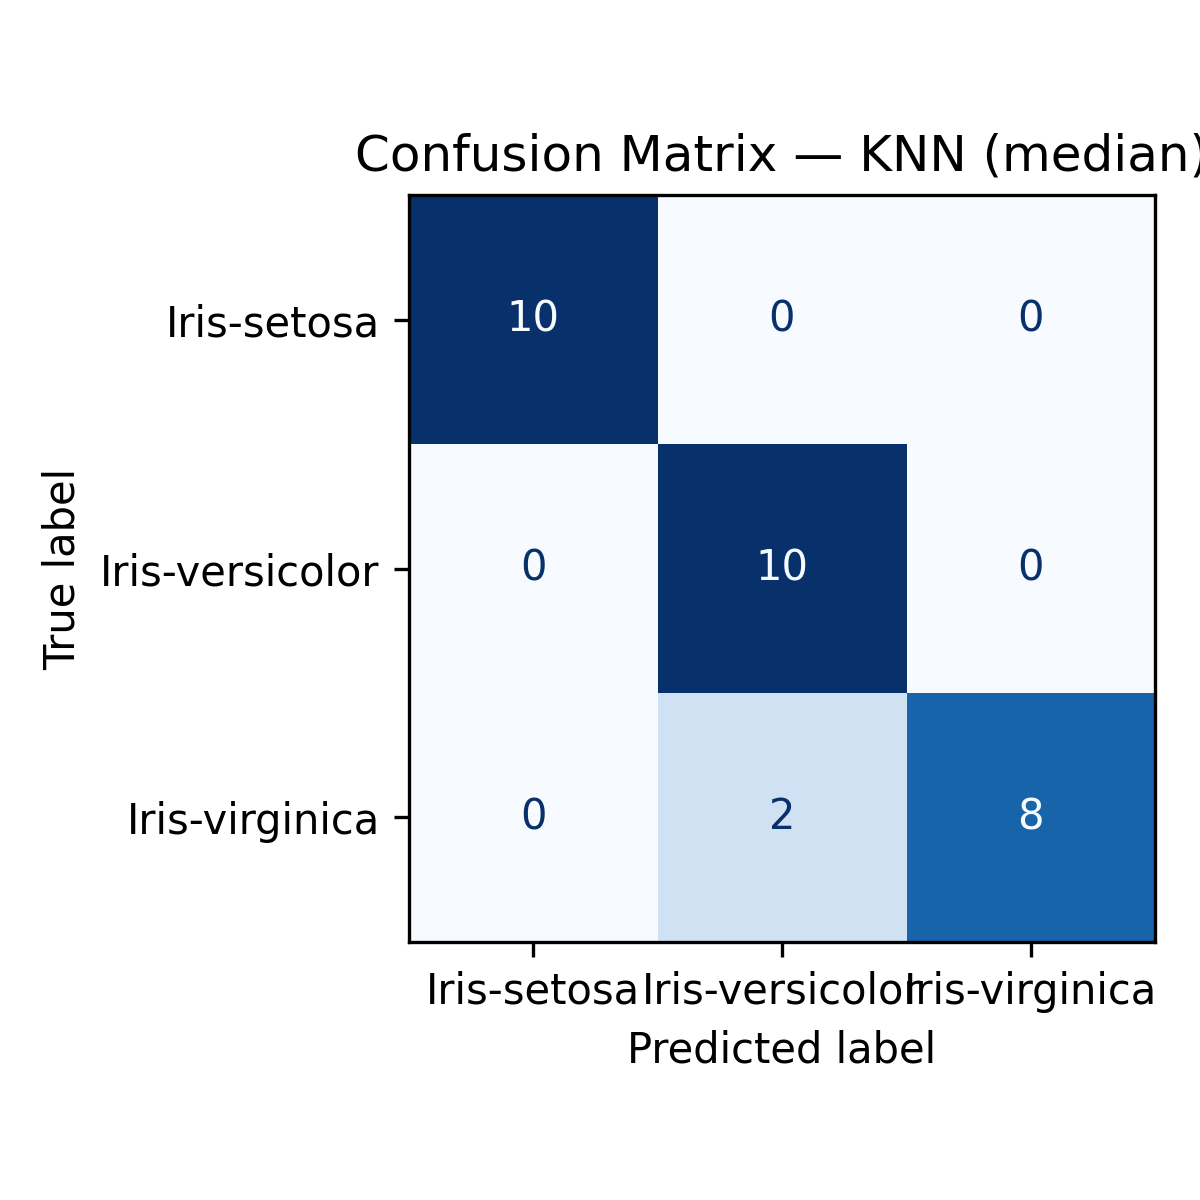
\includegraphics[width=0.22\linewidth]{figures/confmat_median_KNN.png}}\\[0.4em]
    % --- knn ---
    \subfloat[knn--DecisionTree]{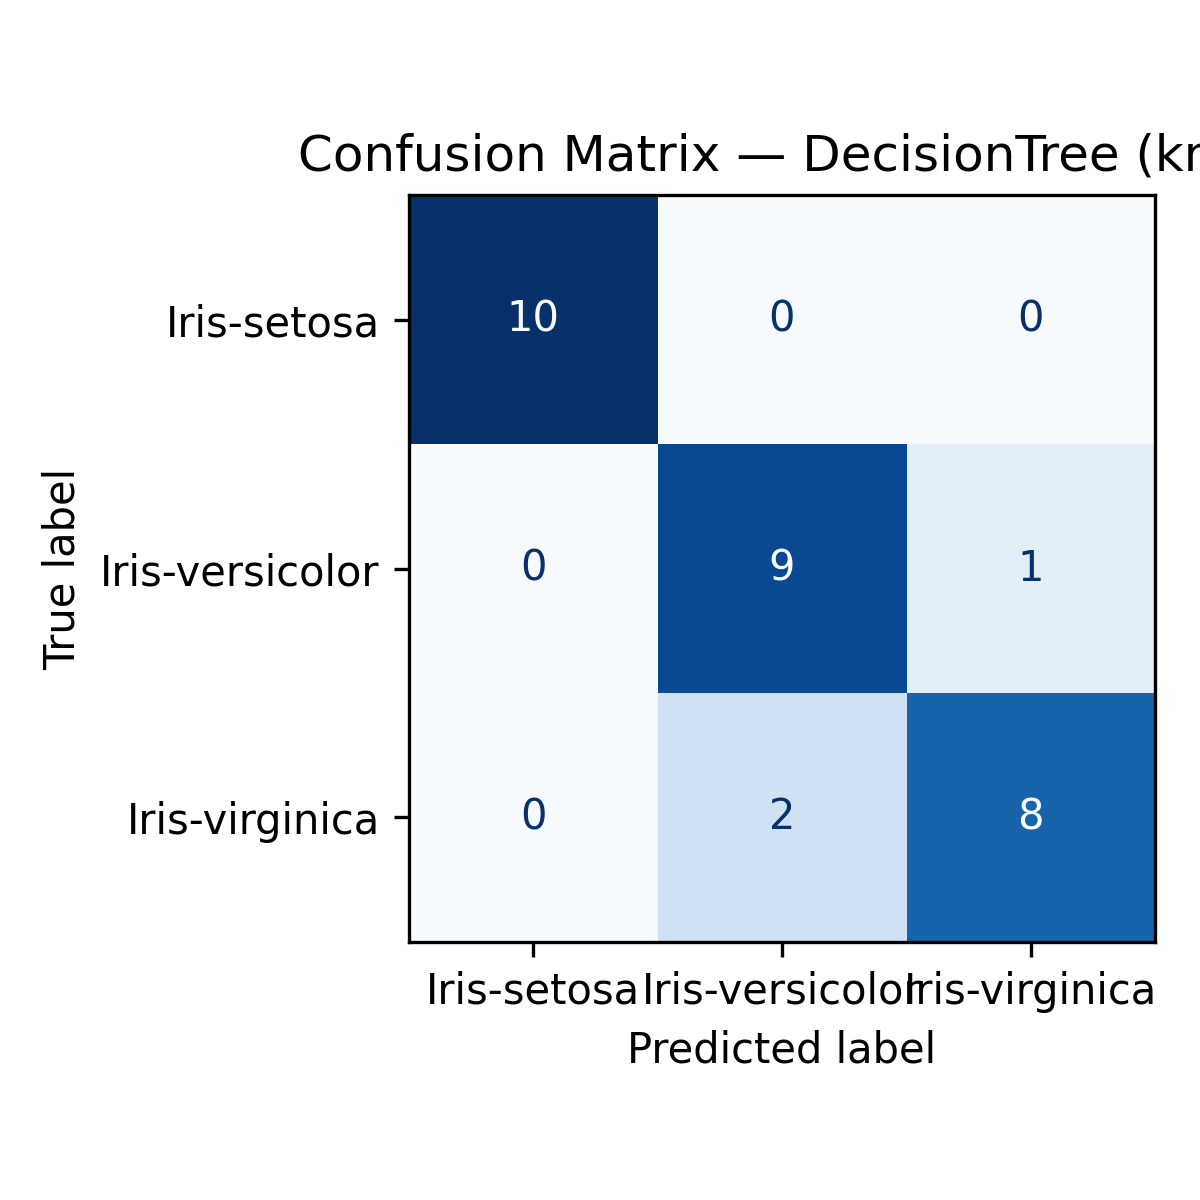
\includegraphics[width=0.22\linewidth]{figures/confmat_knn_DecisionTree.png}}
    \subfloat[knn--LogReg]{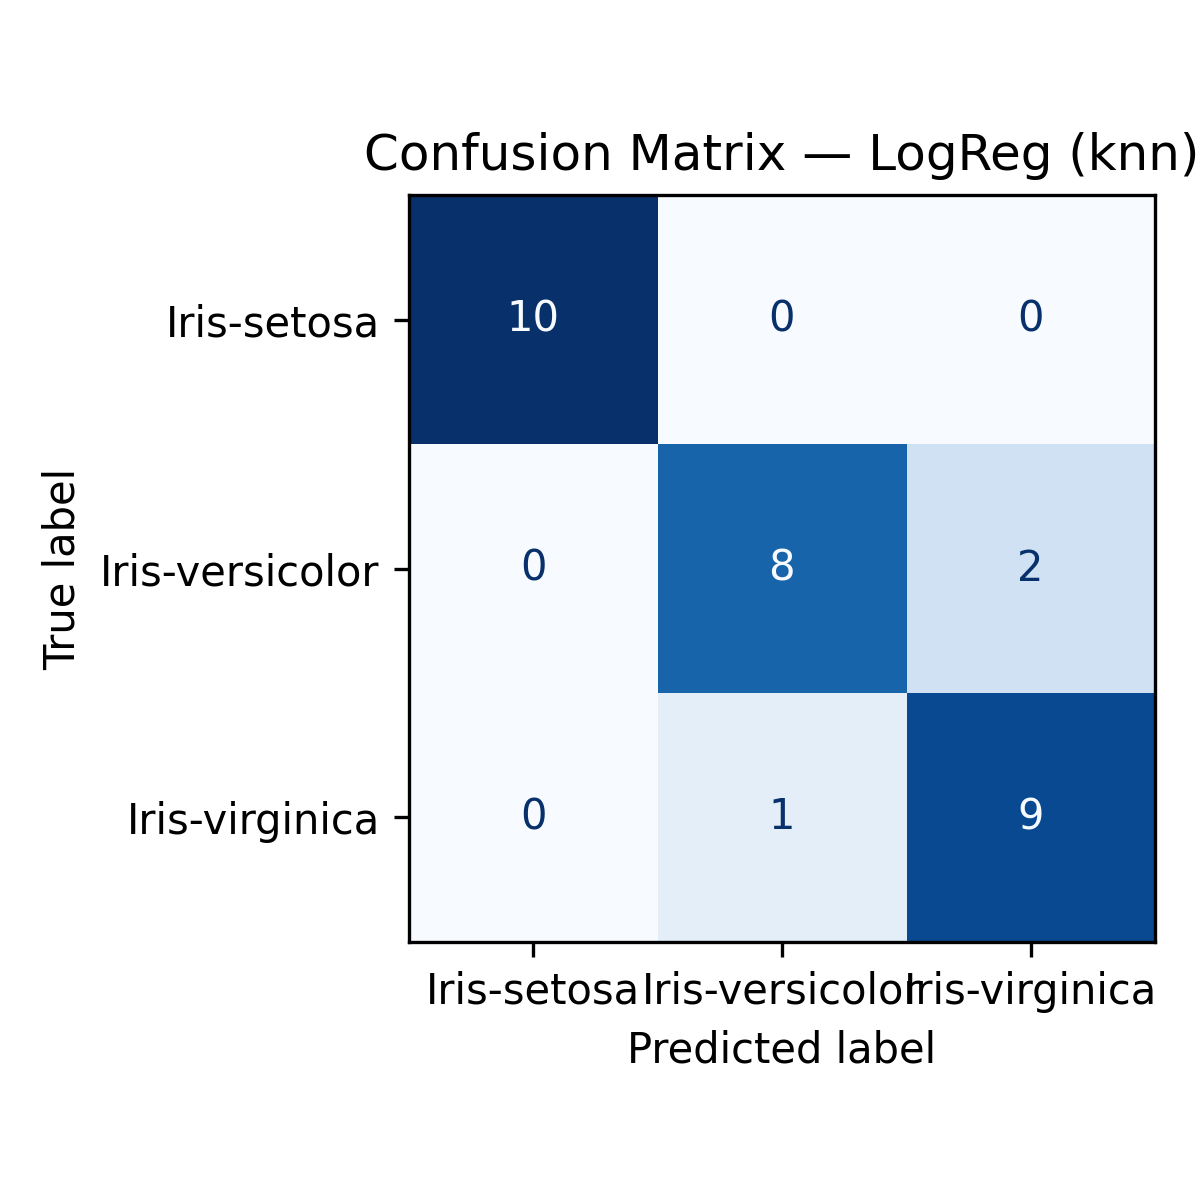
\includegraphics[width=0.22\linewidth]{figures/confmat_knn_LogReg.png}}
    \subfloat[knn--SVM]{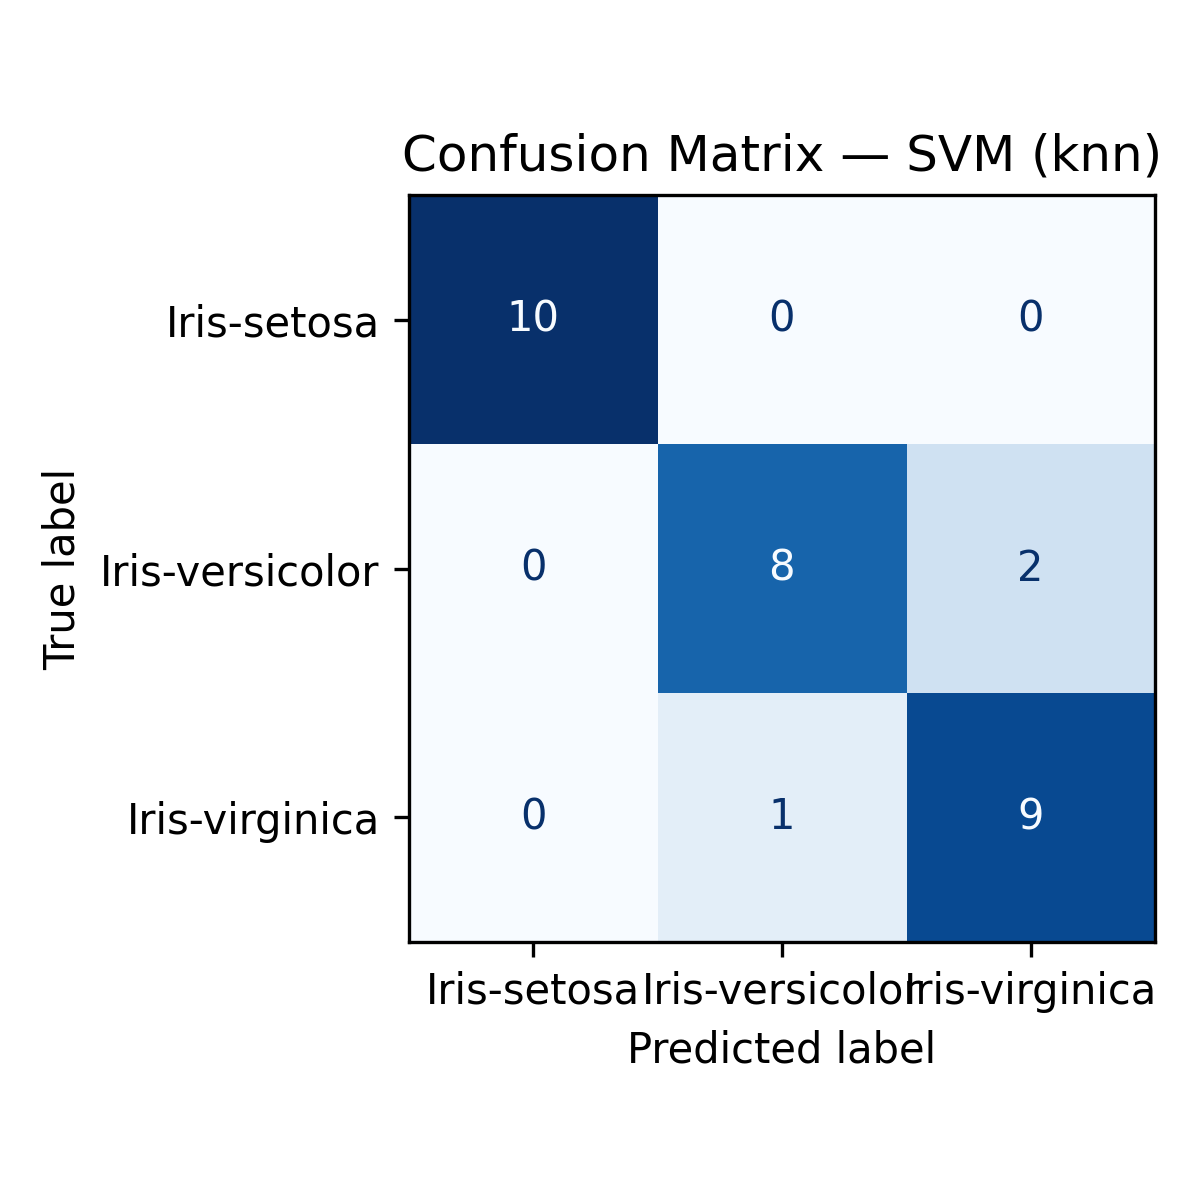
\includegraphics[width=0.22\linewidth]{figures/confmat_knn_SVM.png}}
    \subfloat[knn--KNN]{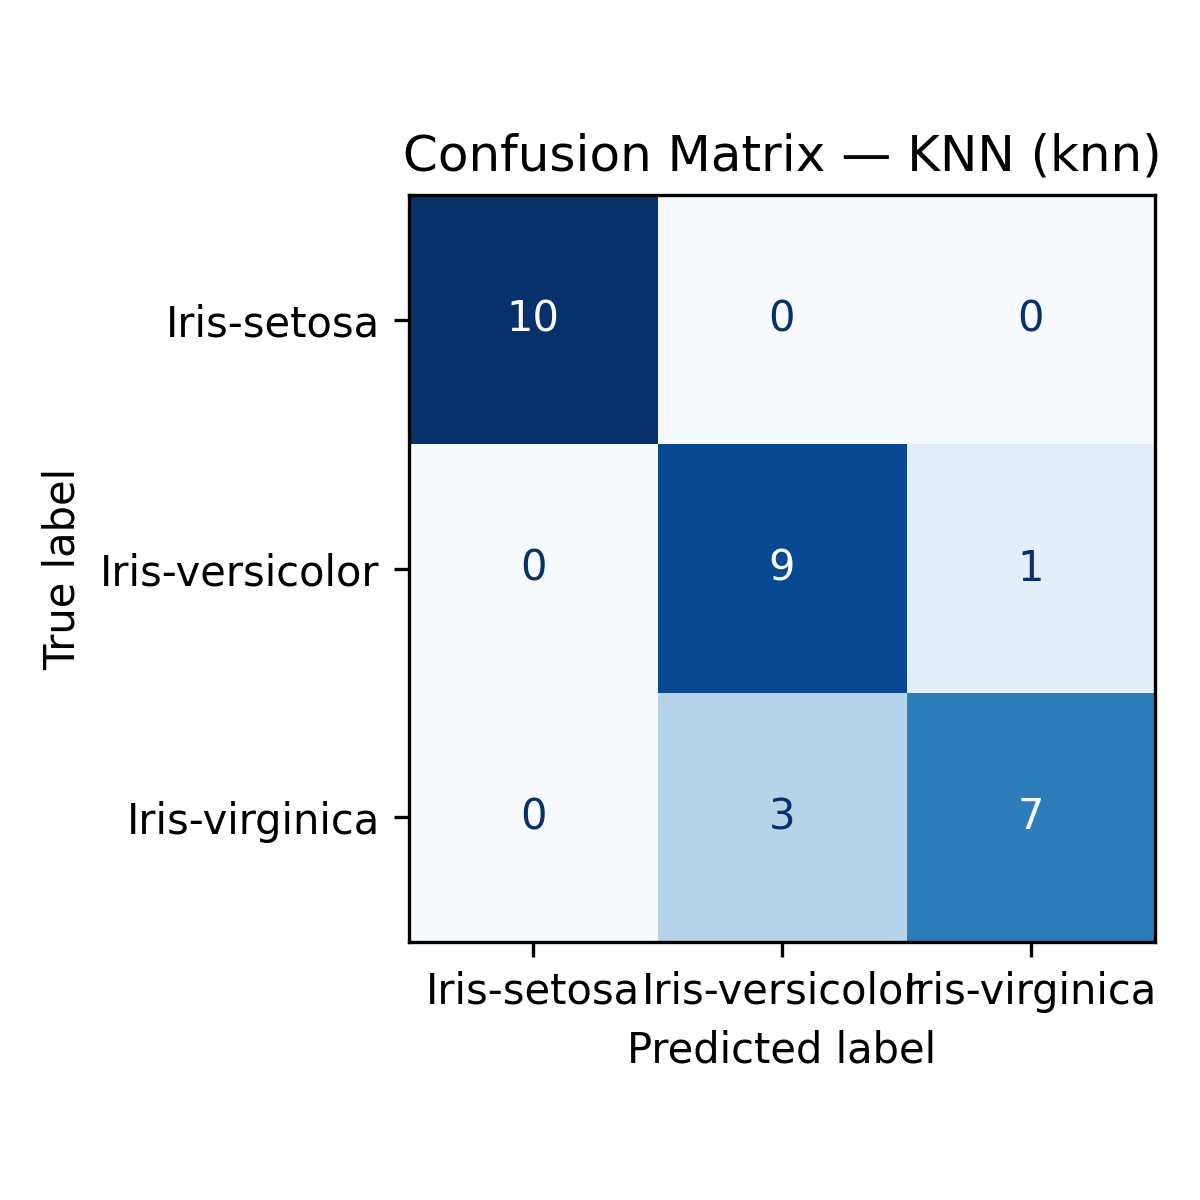
\includegraphics[width=0.22\linewidth]{figures/confmat_knn_KNN.png}}
    \caption{四种缺失值策略与四类分类器的混淆矩阵(共 16 张)}
    \label{fig:all_confmats}
\end{figure}

%--------------------------------------------------
\paragraph{4.2 无监督学习模块(\texttt{task2.py})}
\begin{enumerate}[label=\arabic*)]
    \item \textbf{预处理与标准化}\\
          对 \emph{Mall Customers} 数据集进行三倍 IQR Winsorization、Label Encoding 与 \texttt{StandardScaler}。
    \item \textbf{降维可视化}\\
          使用 \textbf{PCA} 与 \textbf{t-SNE} 将特征映射到二维平面(见图~\ref{fig:pca_tsne_all})。
    \item \textbf{最优簇数确定}\\
          通过 Elbow 与 Silhouette 曲线确定最佳簇数 \(k^\ast=6\)(图~\ref{fig:elbow_silhouette})。
    \item \textbf{聚类算法比较}\\
          在 \(k^\ast\) 下比较 \textbf{K-Means}、\textbf{Agglomerative} 与 \textbf{DBSCAN} 的内部指标。
\end{enumerate}

%----------------- k 选择曲线 -----------------
\begin{figure}[htbp]
    \centering
    \subfloat[Elbow]{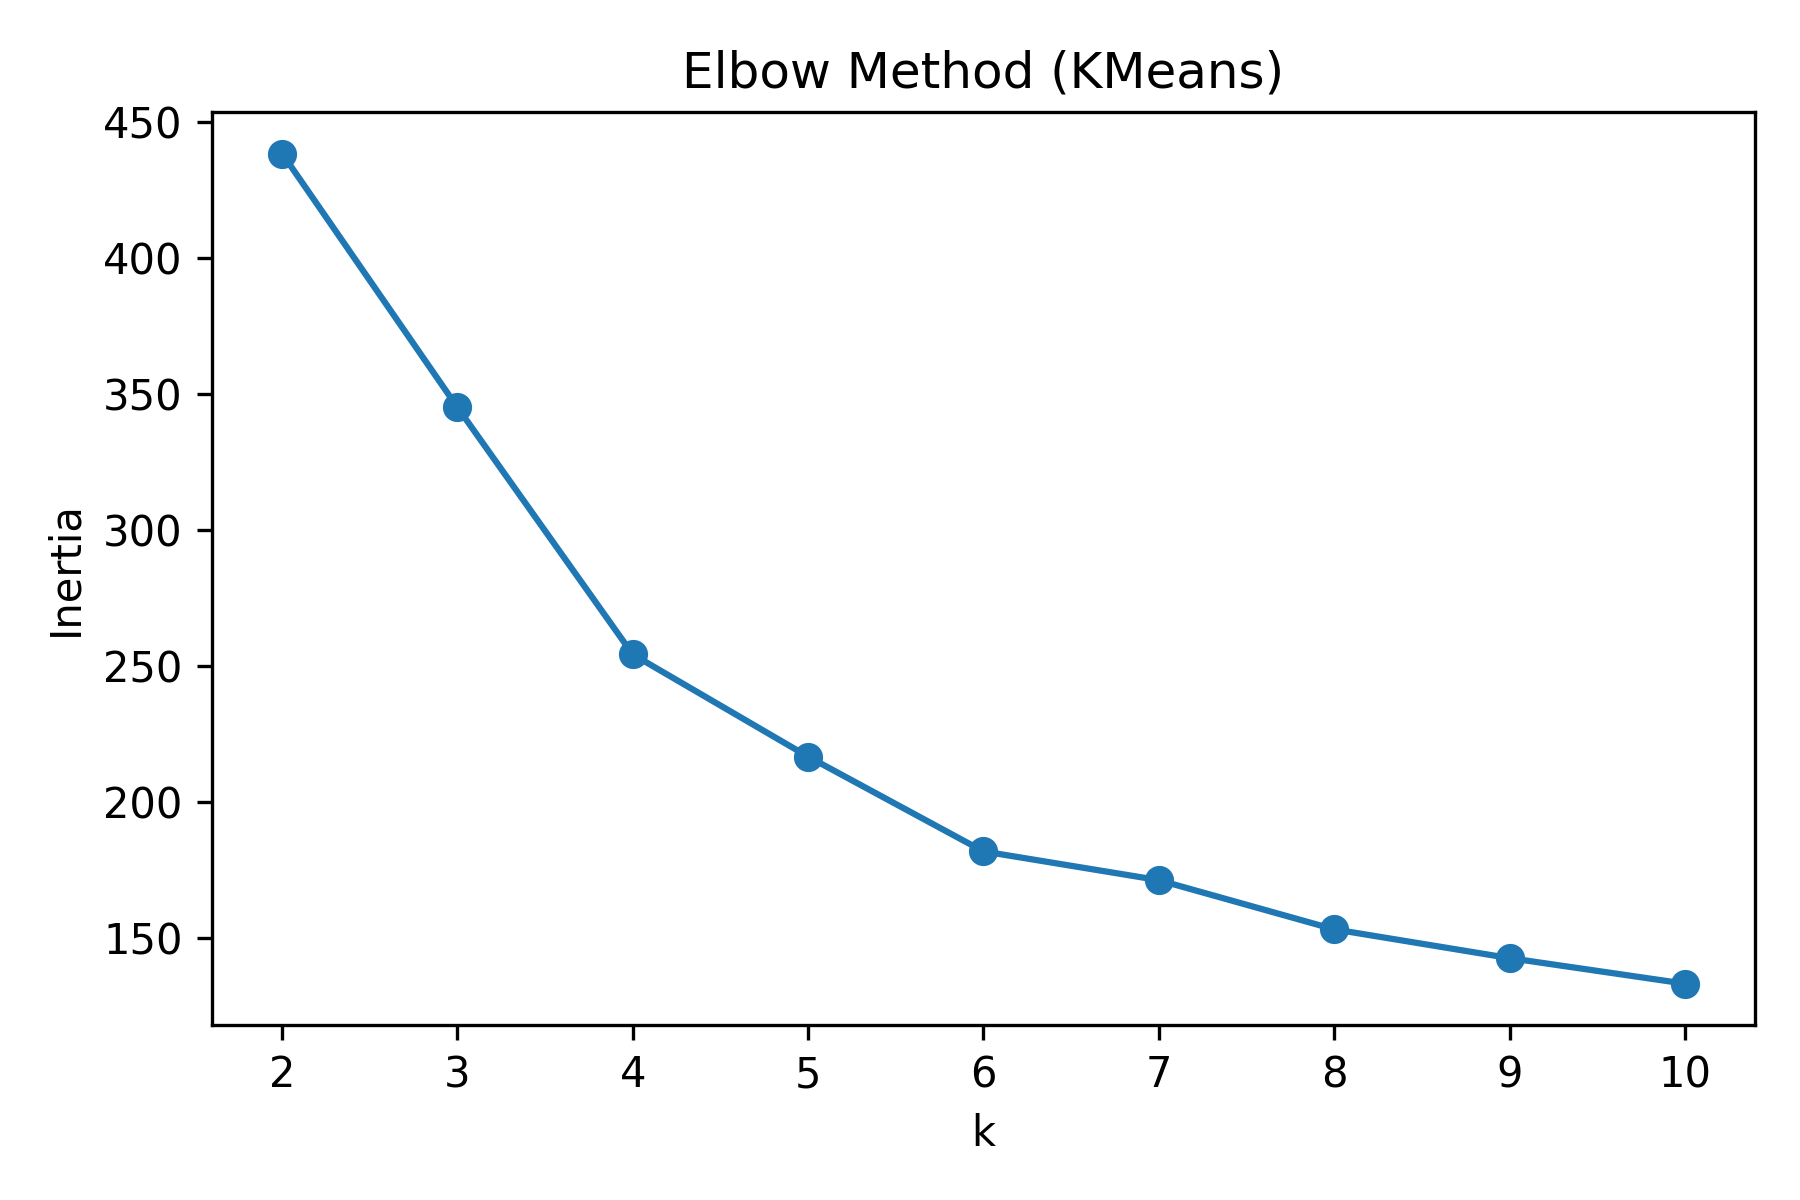
\includegraphics[width=0.45\linewidth]{figures2/elbow.png}}
    \hfill
    \subfloat[Silhouette]{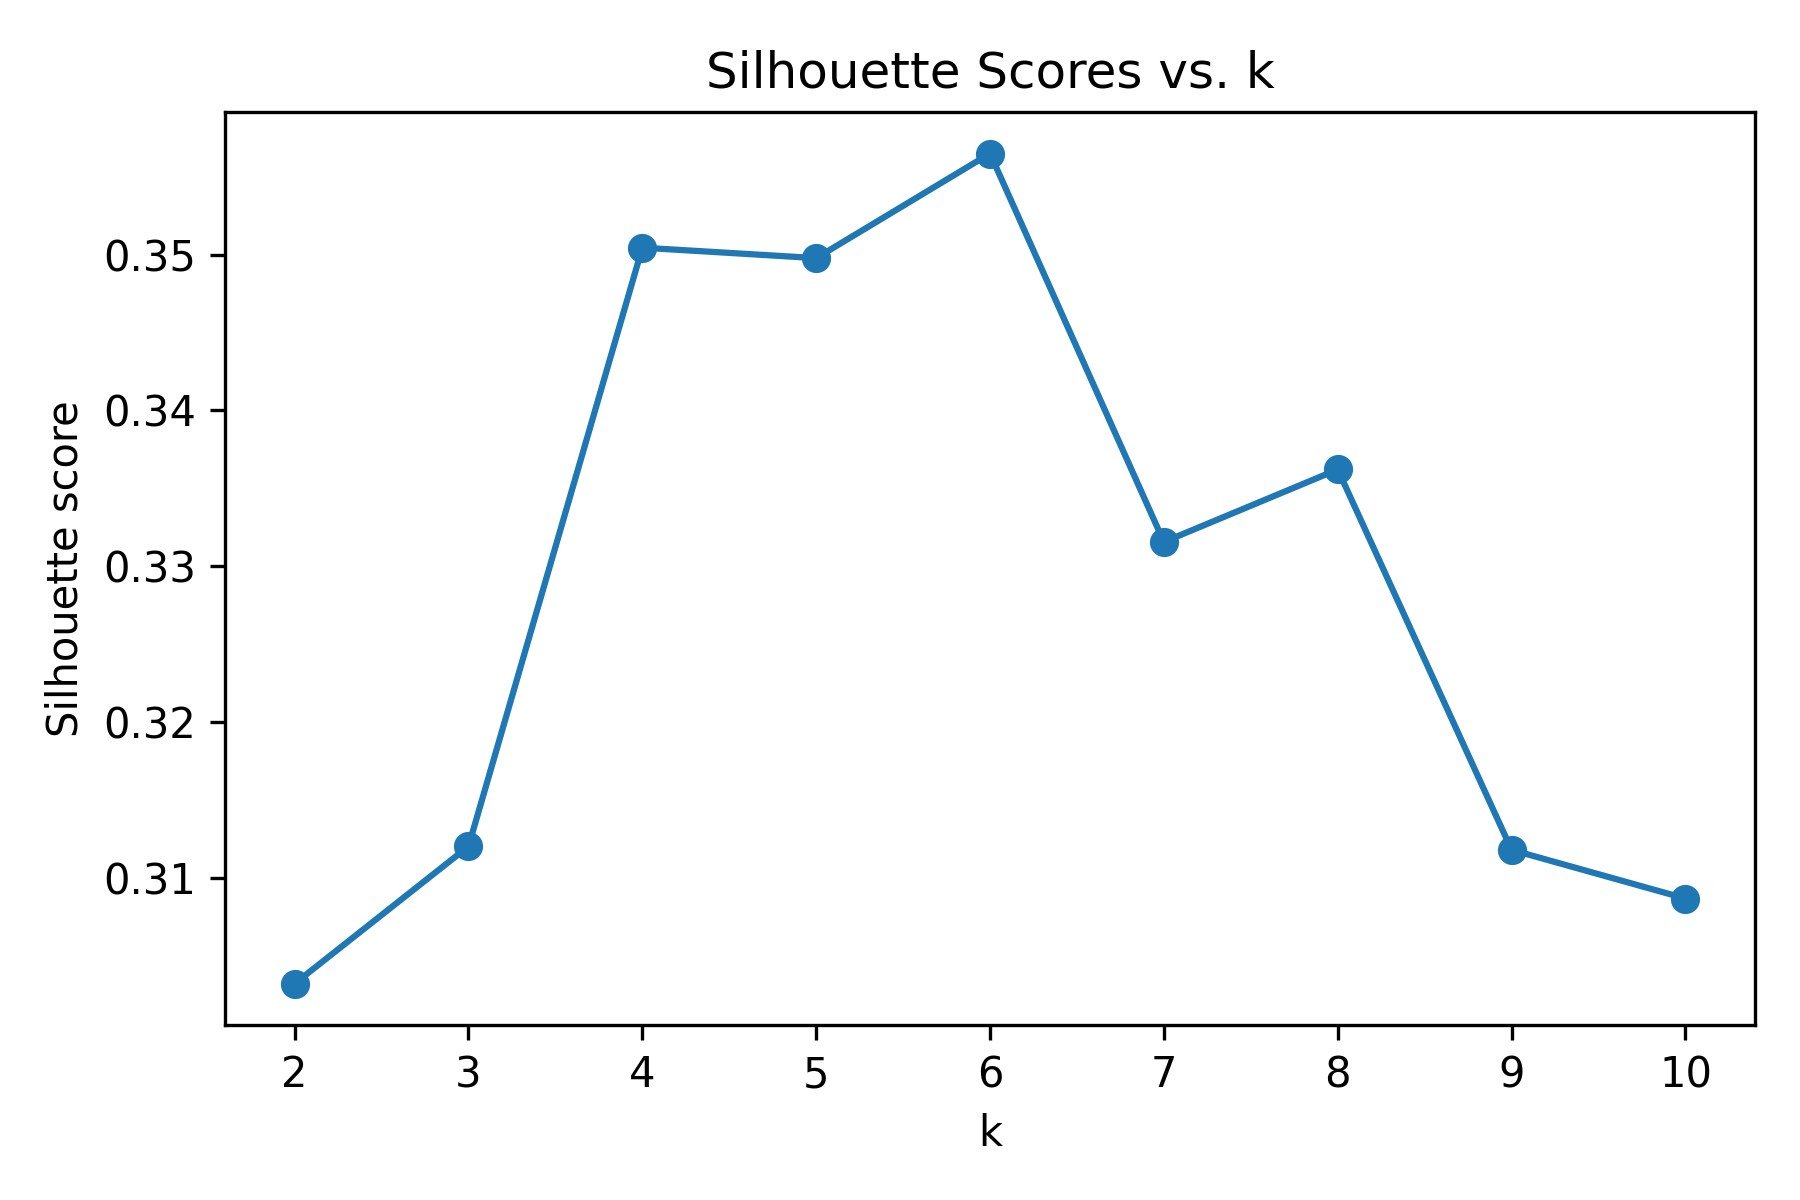
\includegraphics[width=0.45\linewidth]{figures2/silhouette_curve.png}}
    \caption{K-Means 不同 \(k\) 下的惯性与轮廓系数}
    \label{fig:elbow_silhouette}
\end{figure}

%----------------- 特征分布与散点 -----------------
\begin{figure}[htbp]
    \centering
    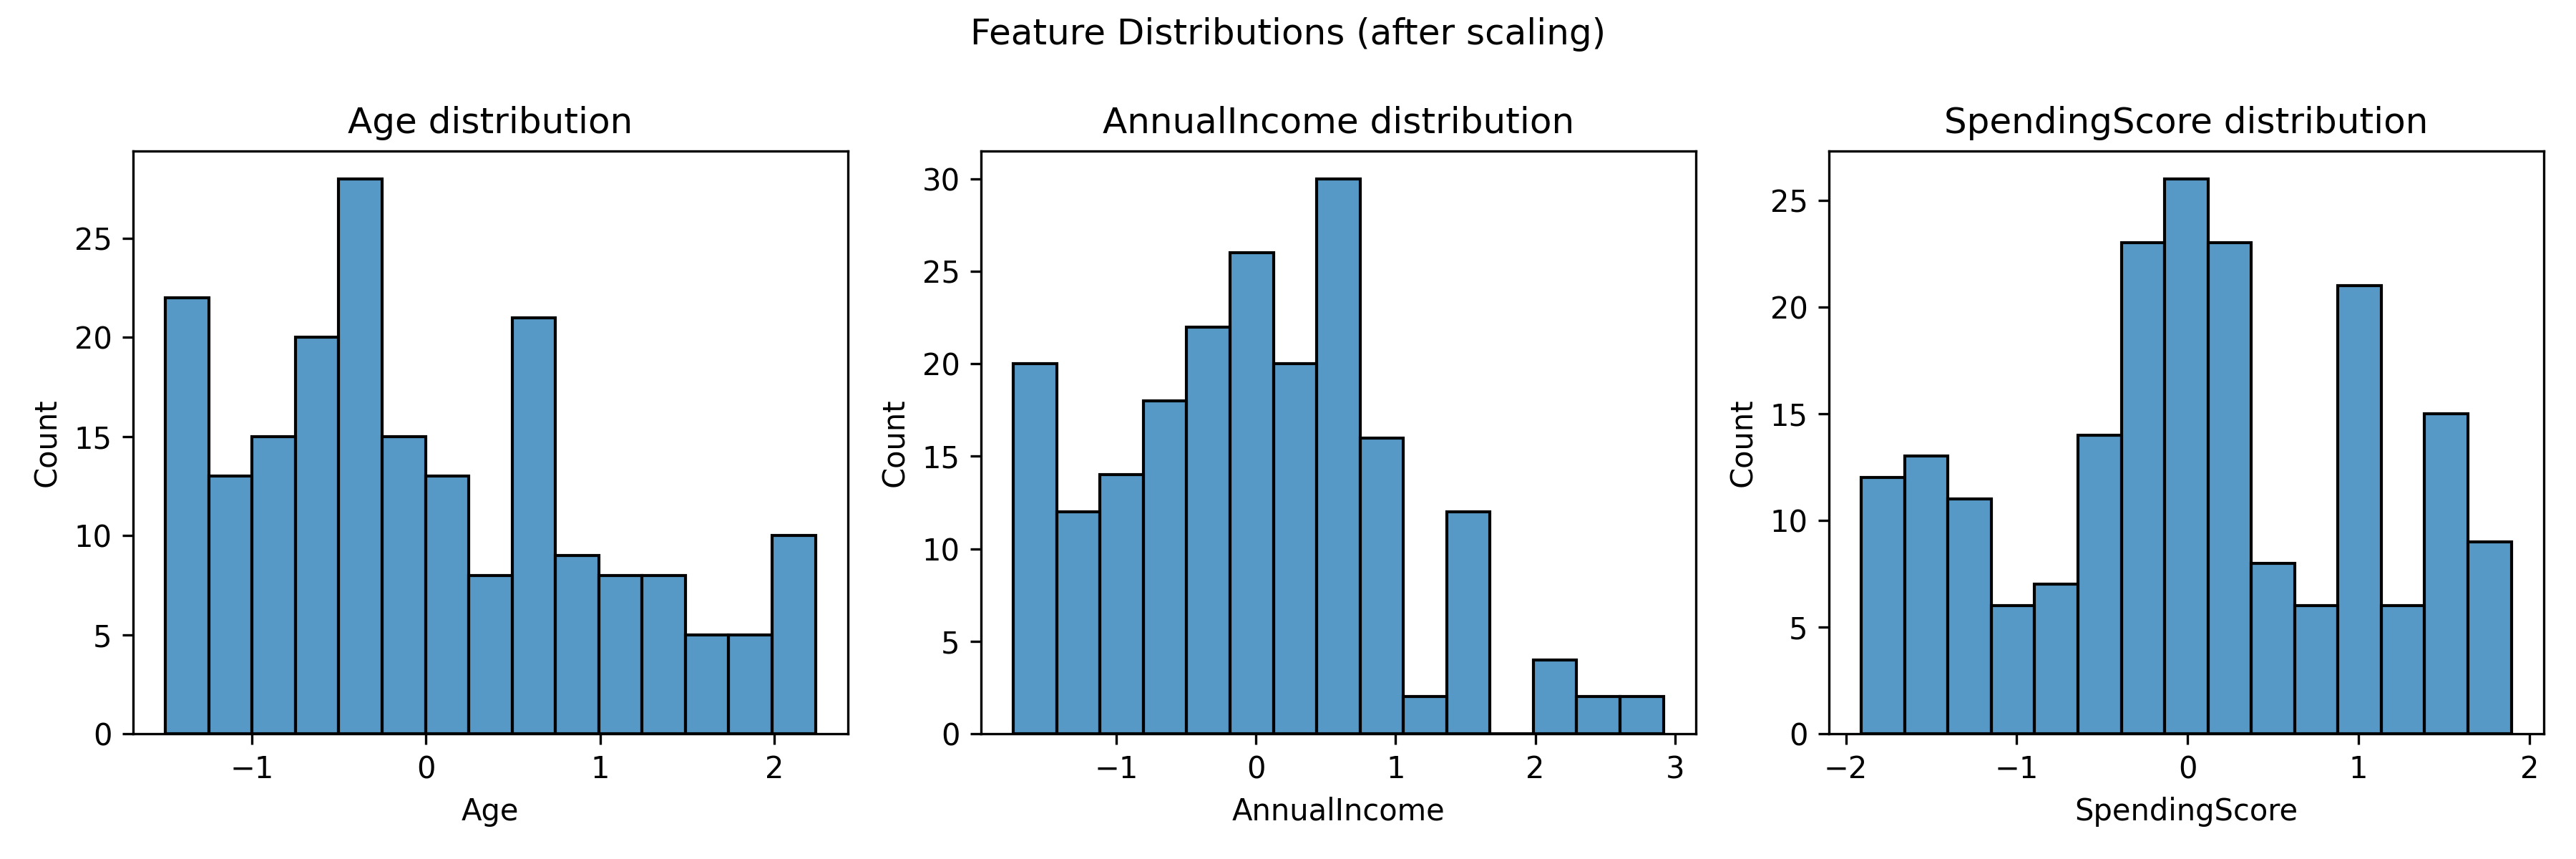
\includegraphics[width=\linewidth]{figures2/feature_hist.png}
    \caption{Age, Annual Income, Spending Score 的标准化直方图}
    \label{fig:feature_hist}
\end{figure}

\begin{figure}[htbp]
    \centering
    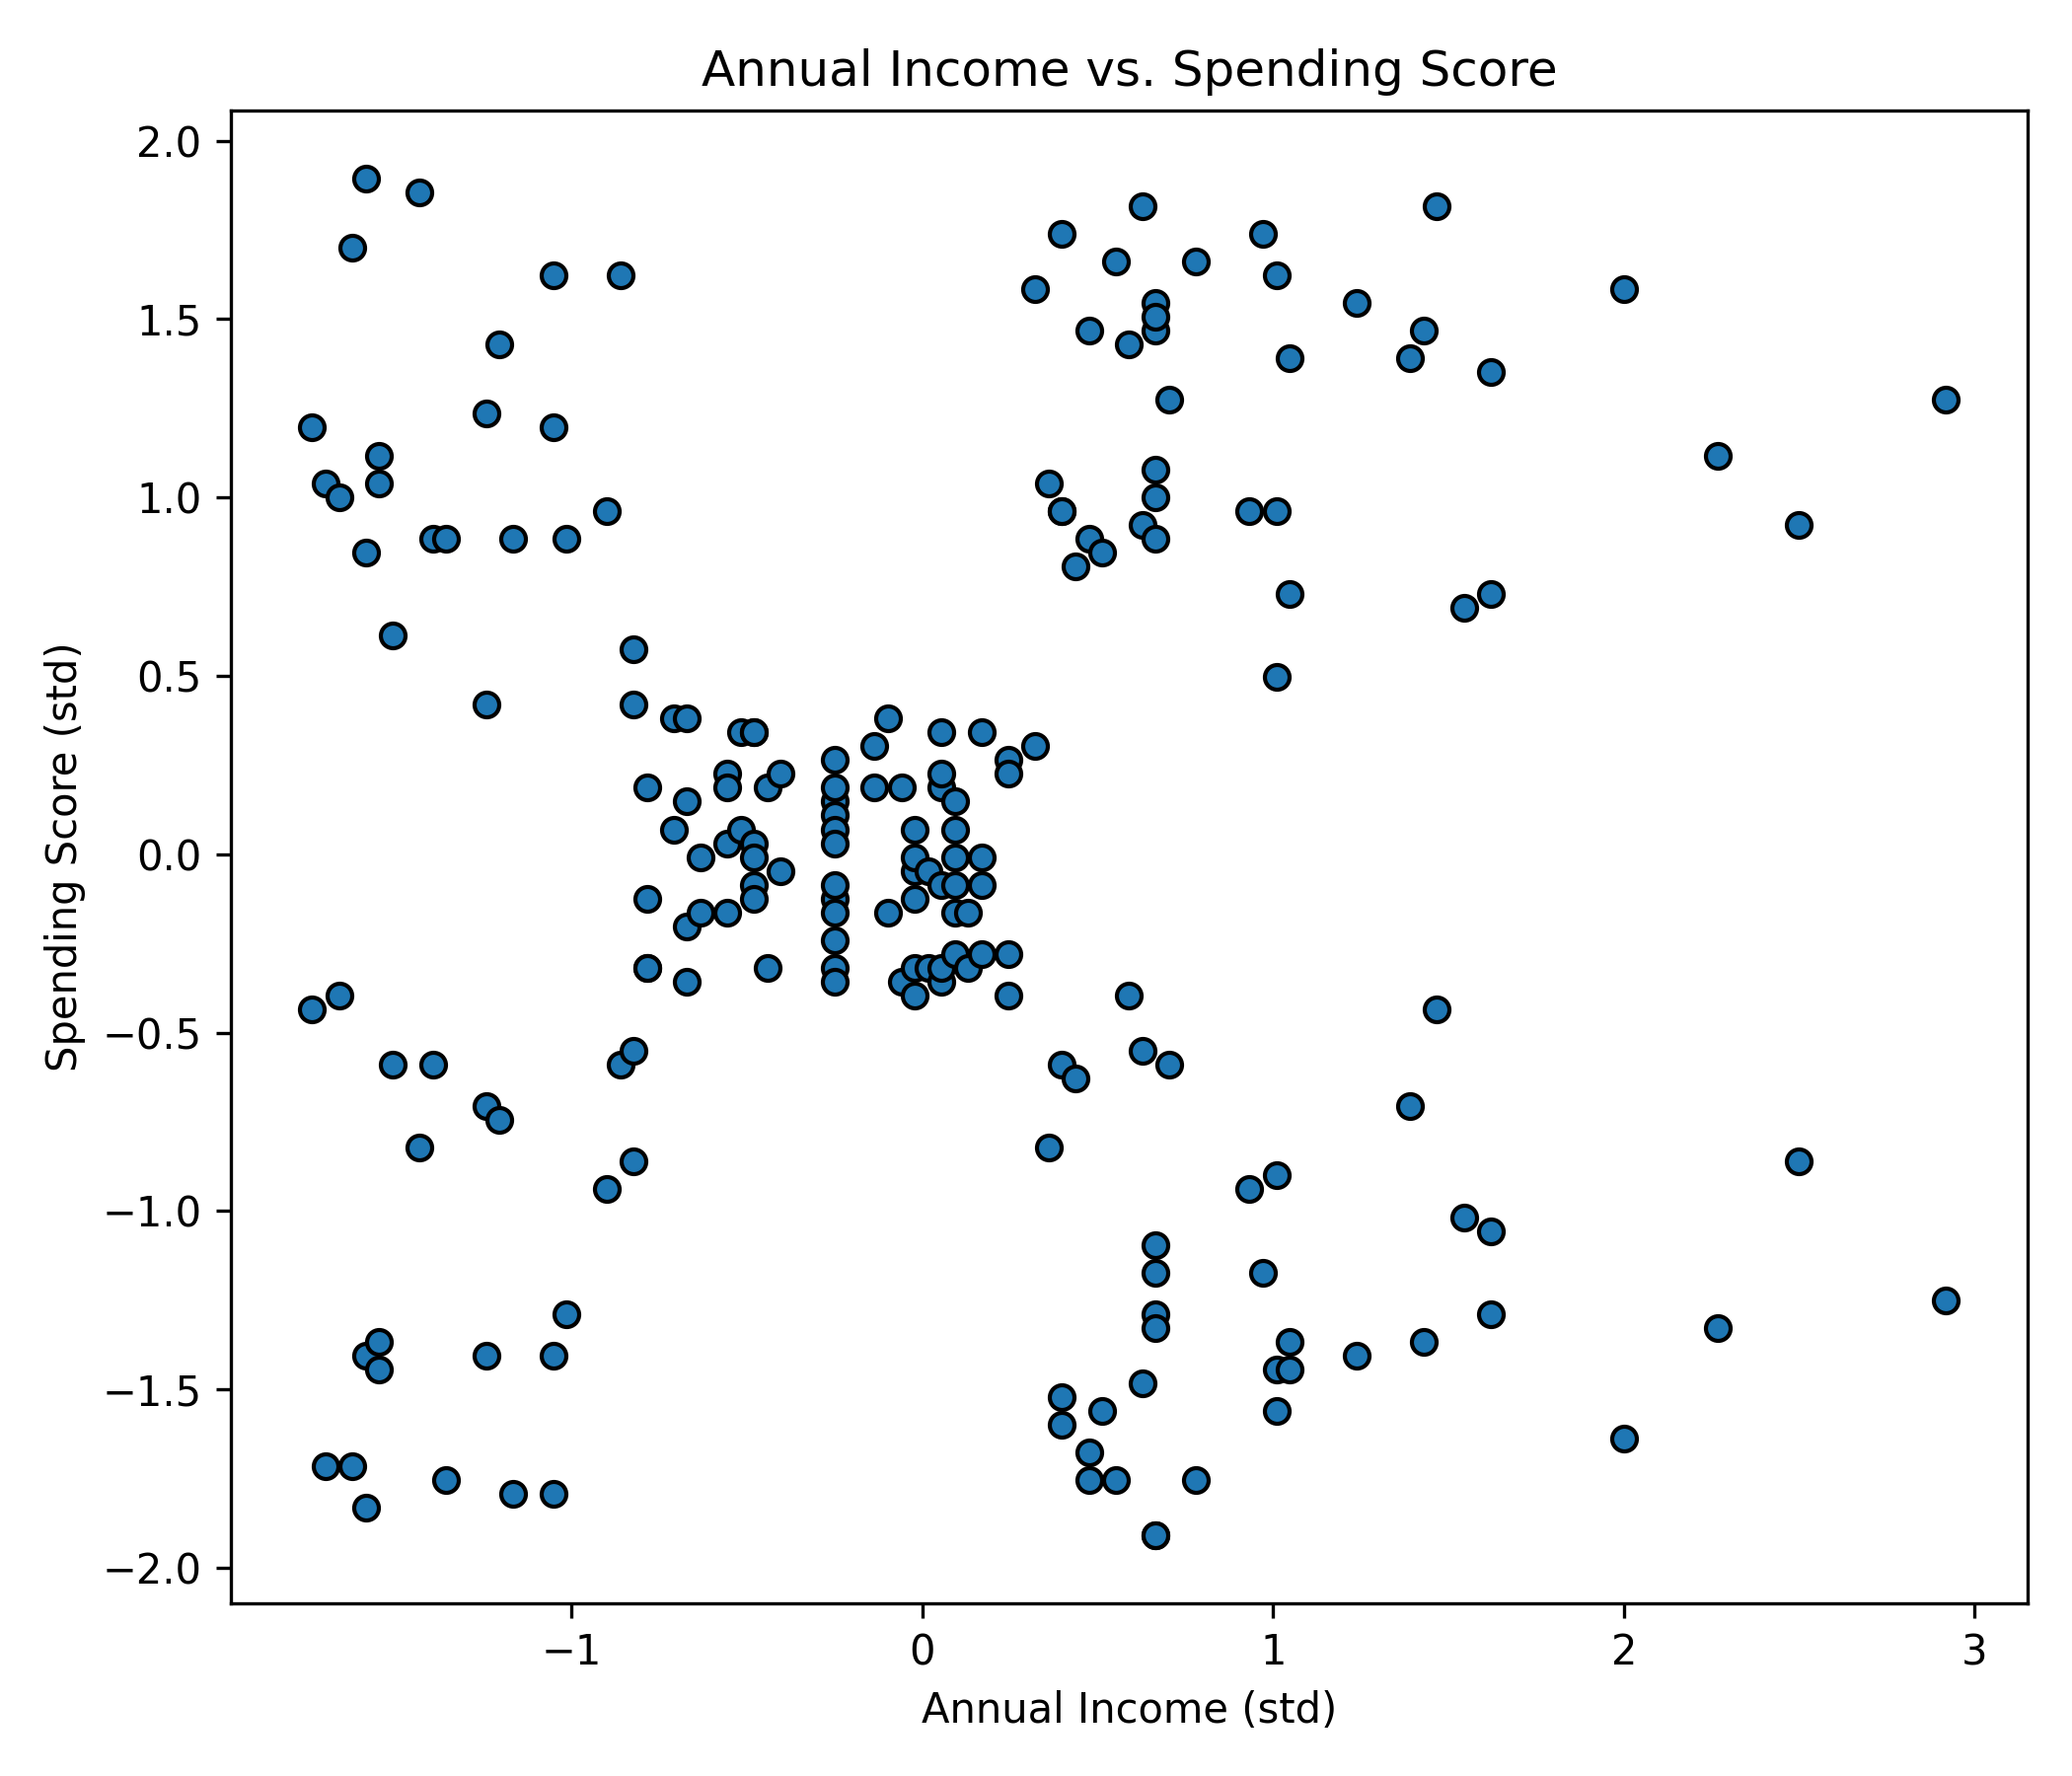
\includegraphics[width=0.6\linewidth]{figures2/income_vs_score.png}
    \caption{Annual Income 与 Spending Score 散点图}
    \label{fig:income_vs_score}
\end{figure}

%----------------- 聚类结果:PCA 与 t-SNE -----------------
\begin{figure}[htbp]
    \centering
    \subfloat[PCA--KMeans]{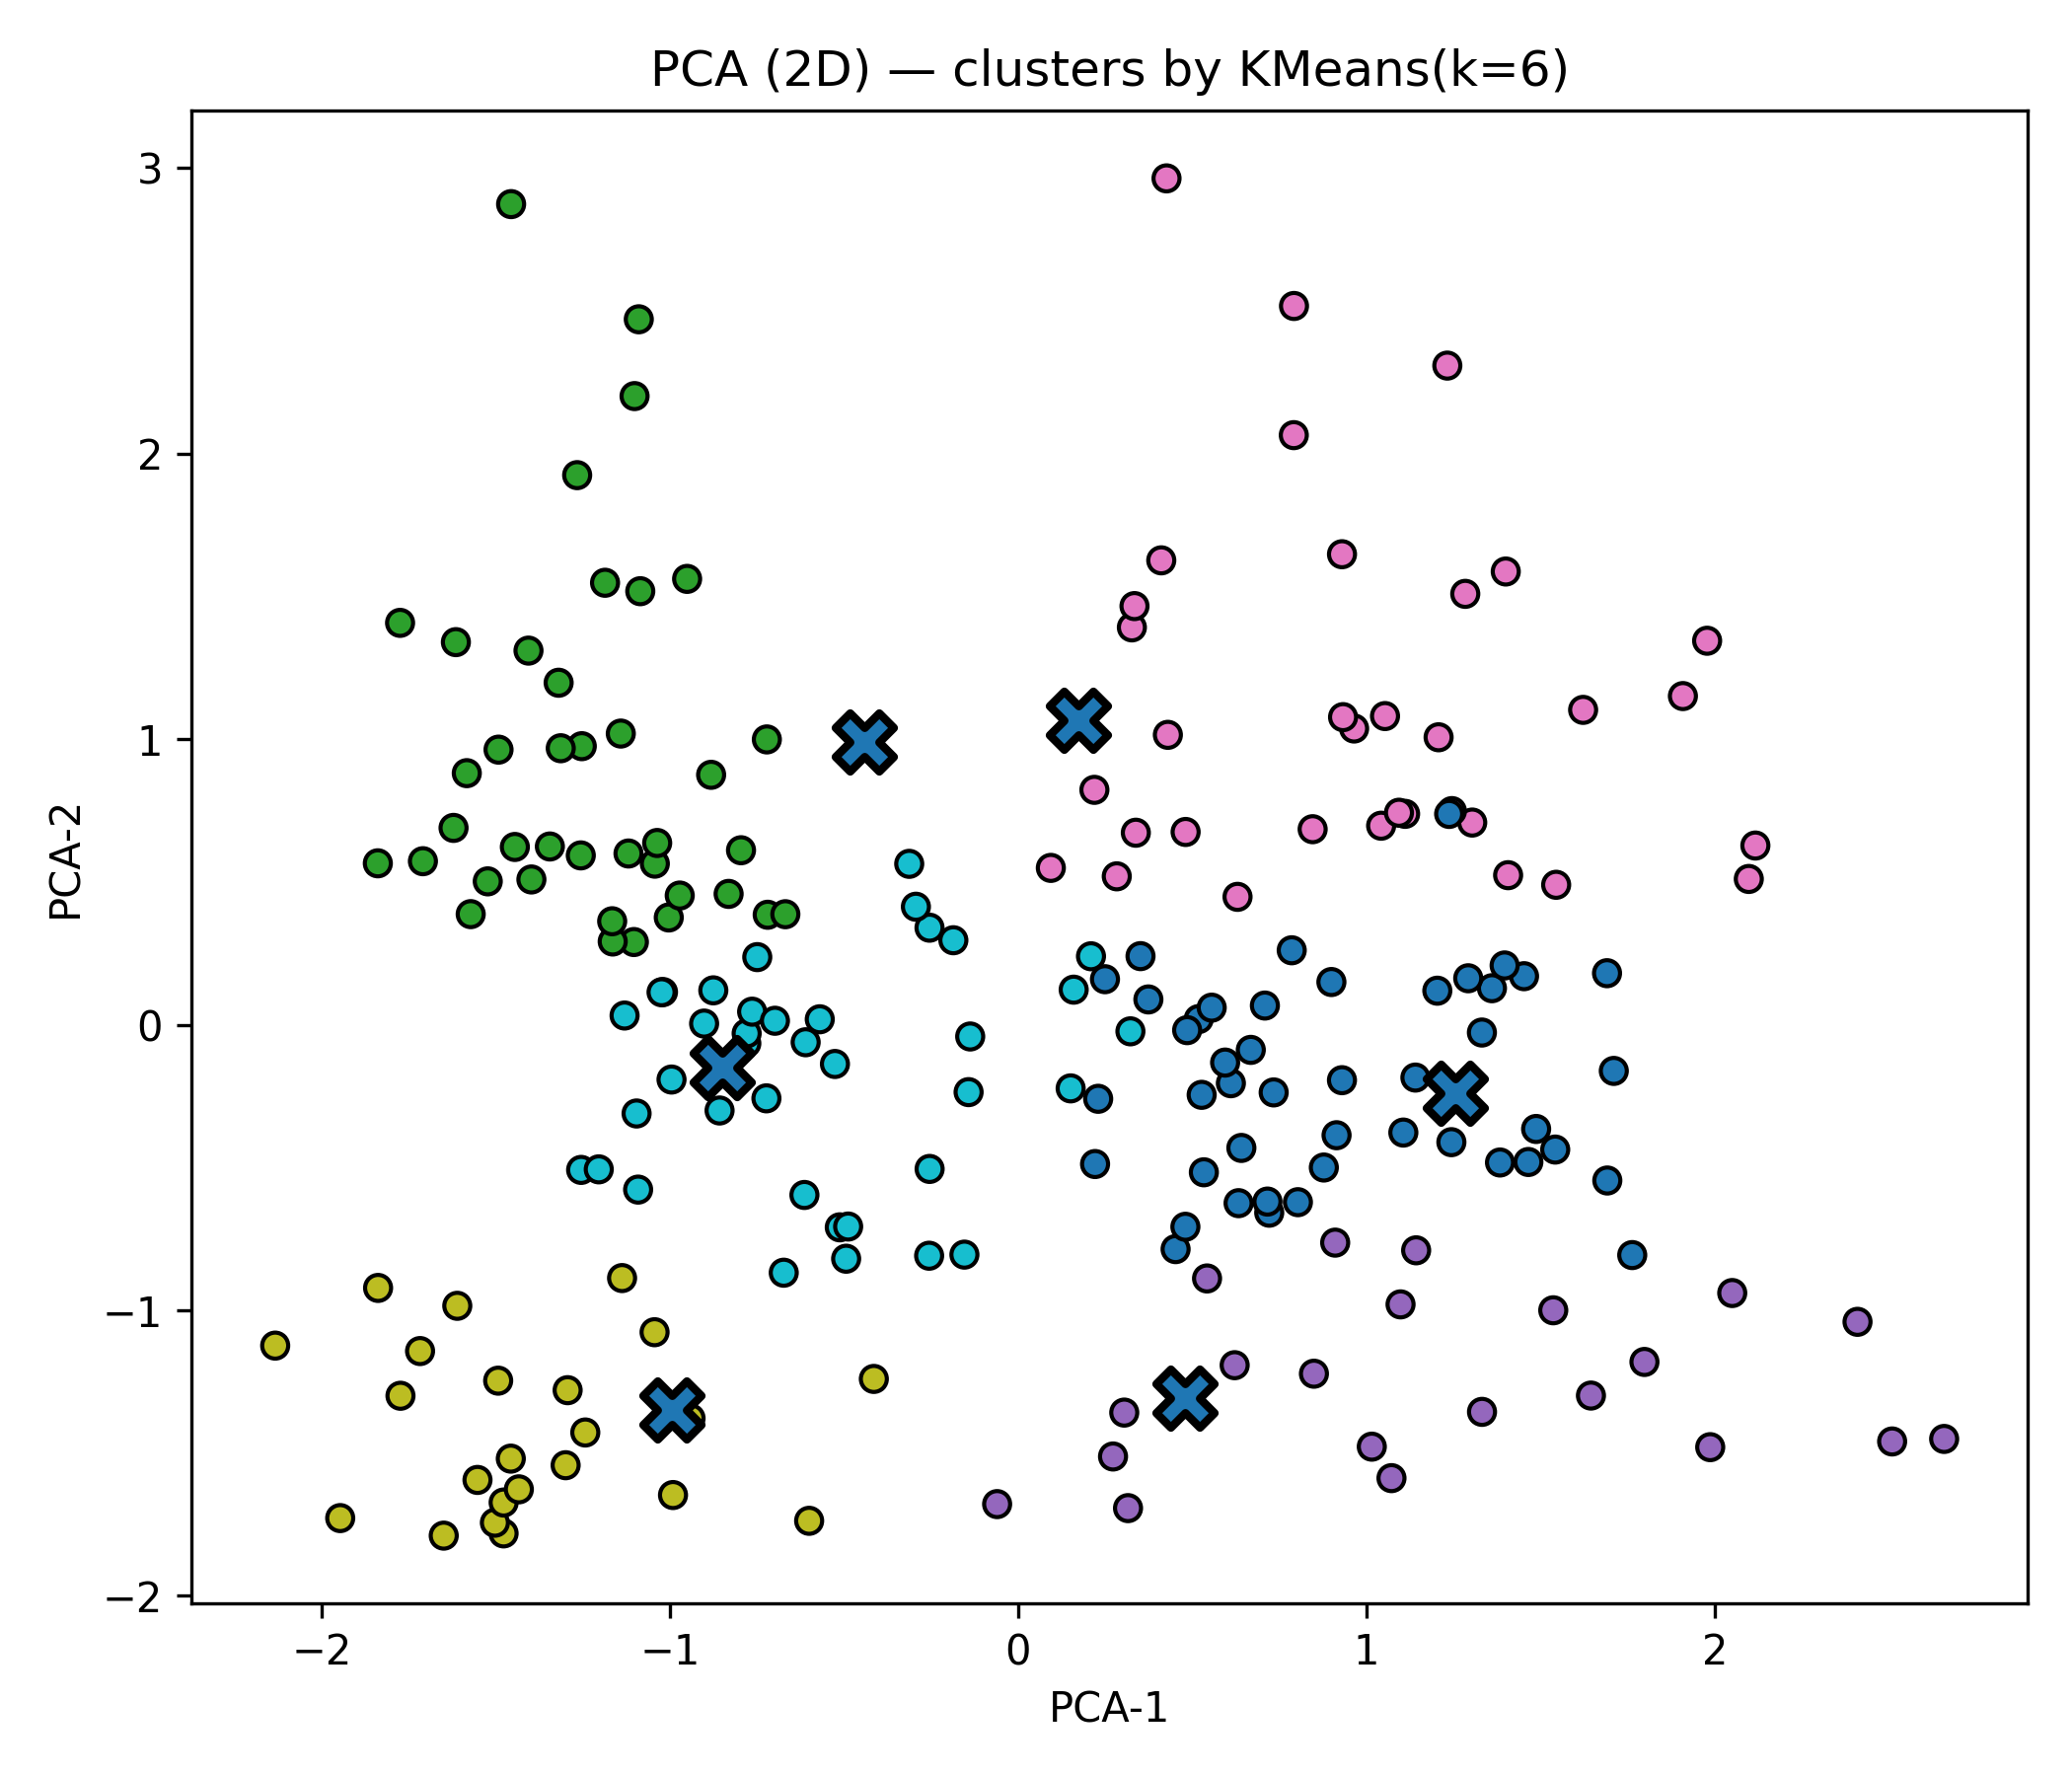
\includegraphics[width=0.3\linewidth]{figures2/pca_kmeans.png}}
    \hfill
    \subfloat[PCA--Agglomerative]{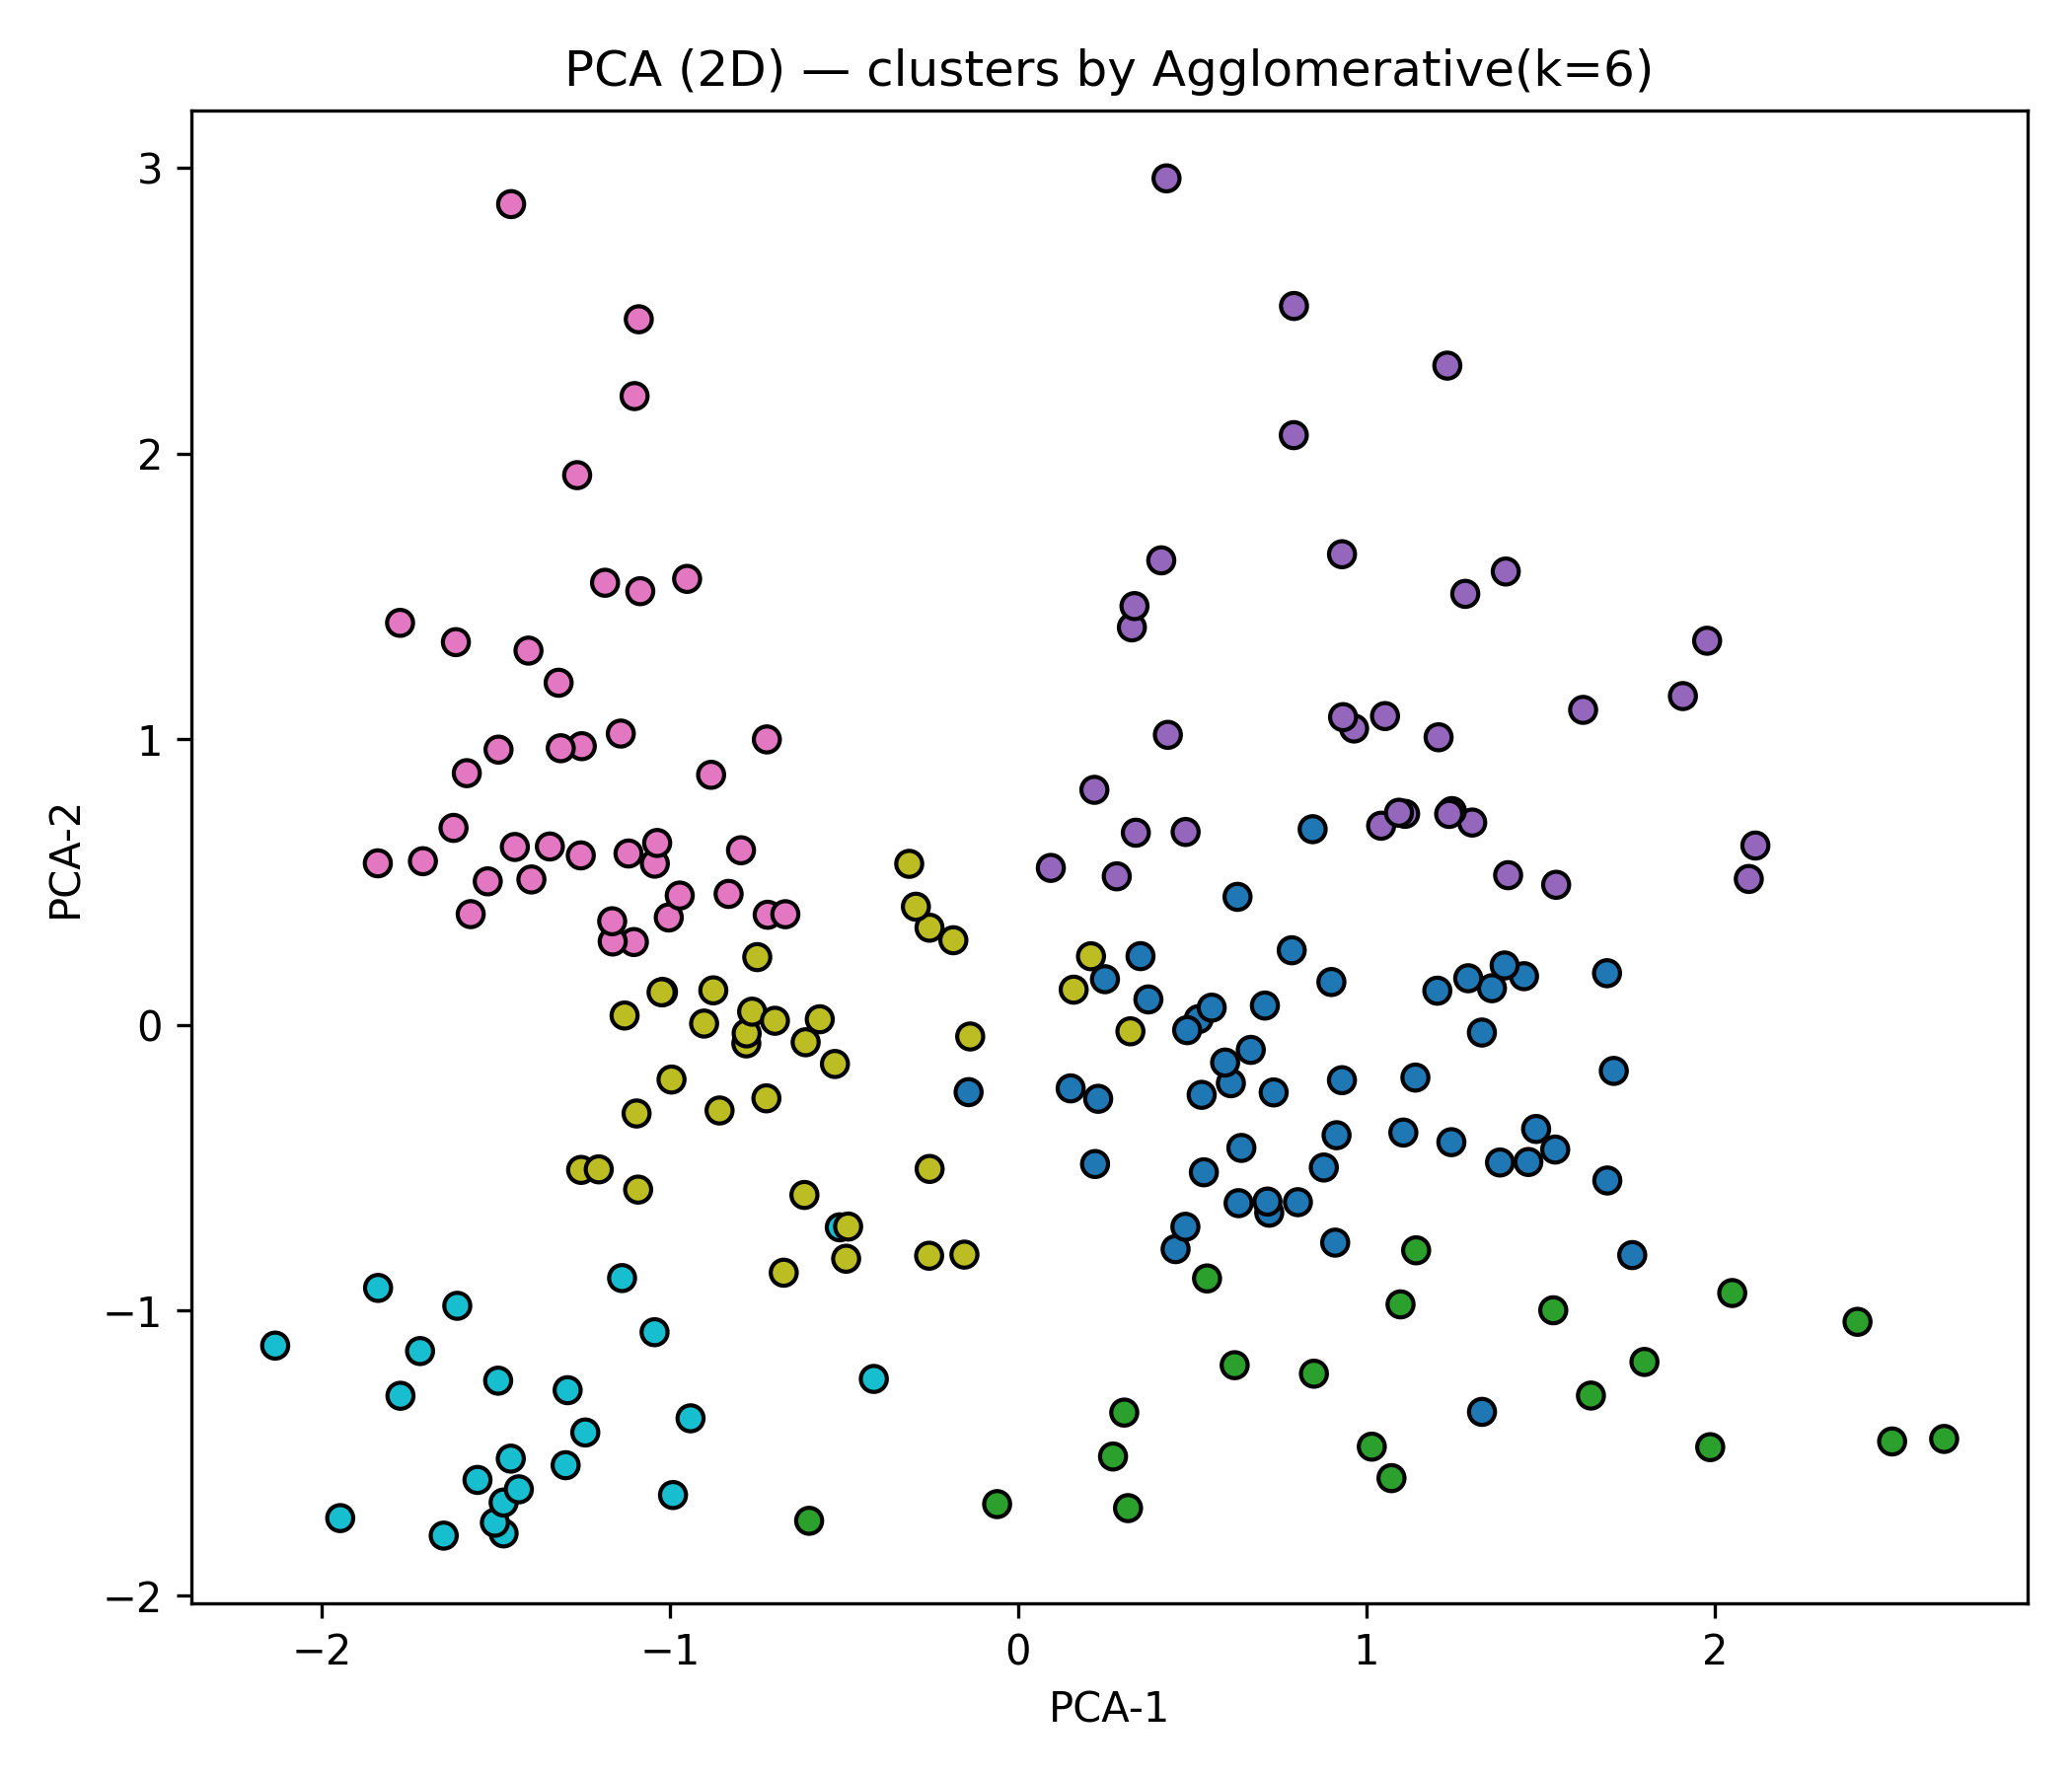
\includegraphics[width=0.3\linewidth]{figures2/pca_agglomerative.png}}
    \hfill
    \subfloat[PCA--DBSCAN]{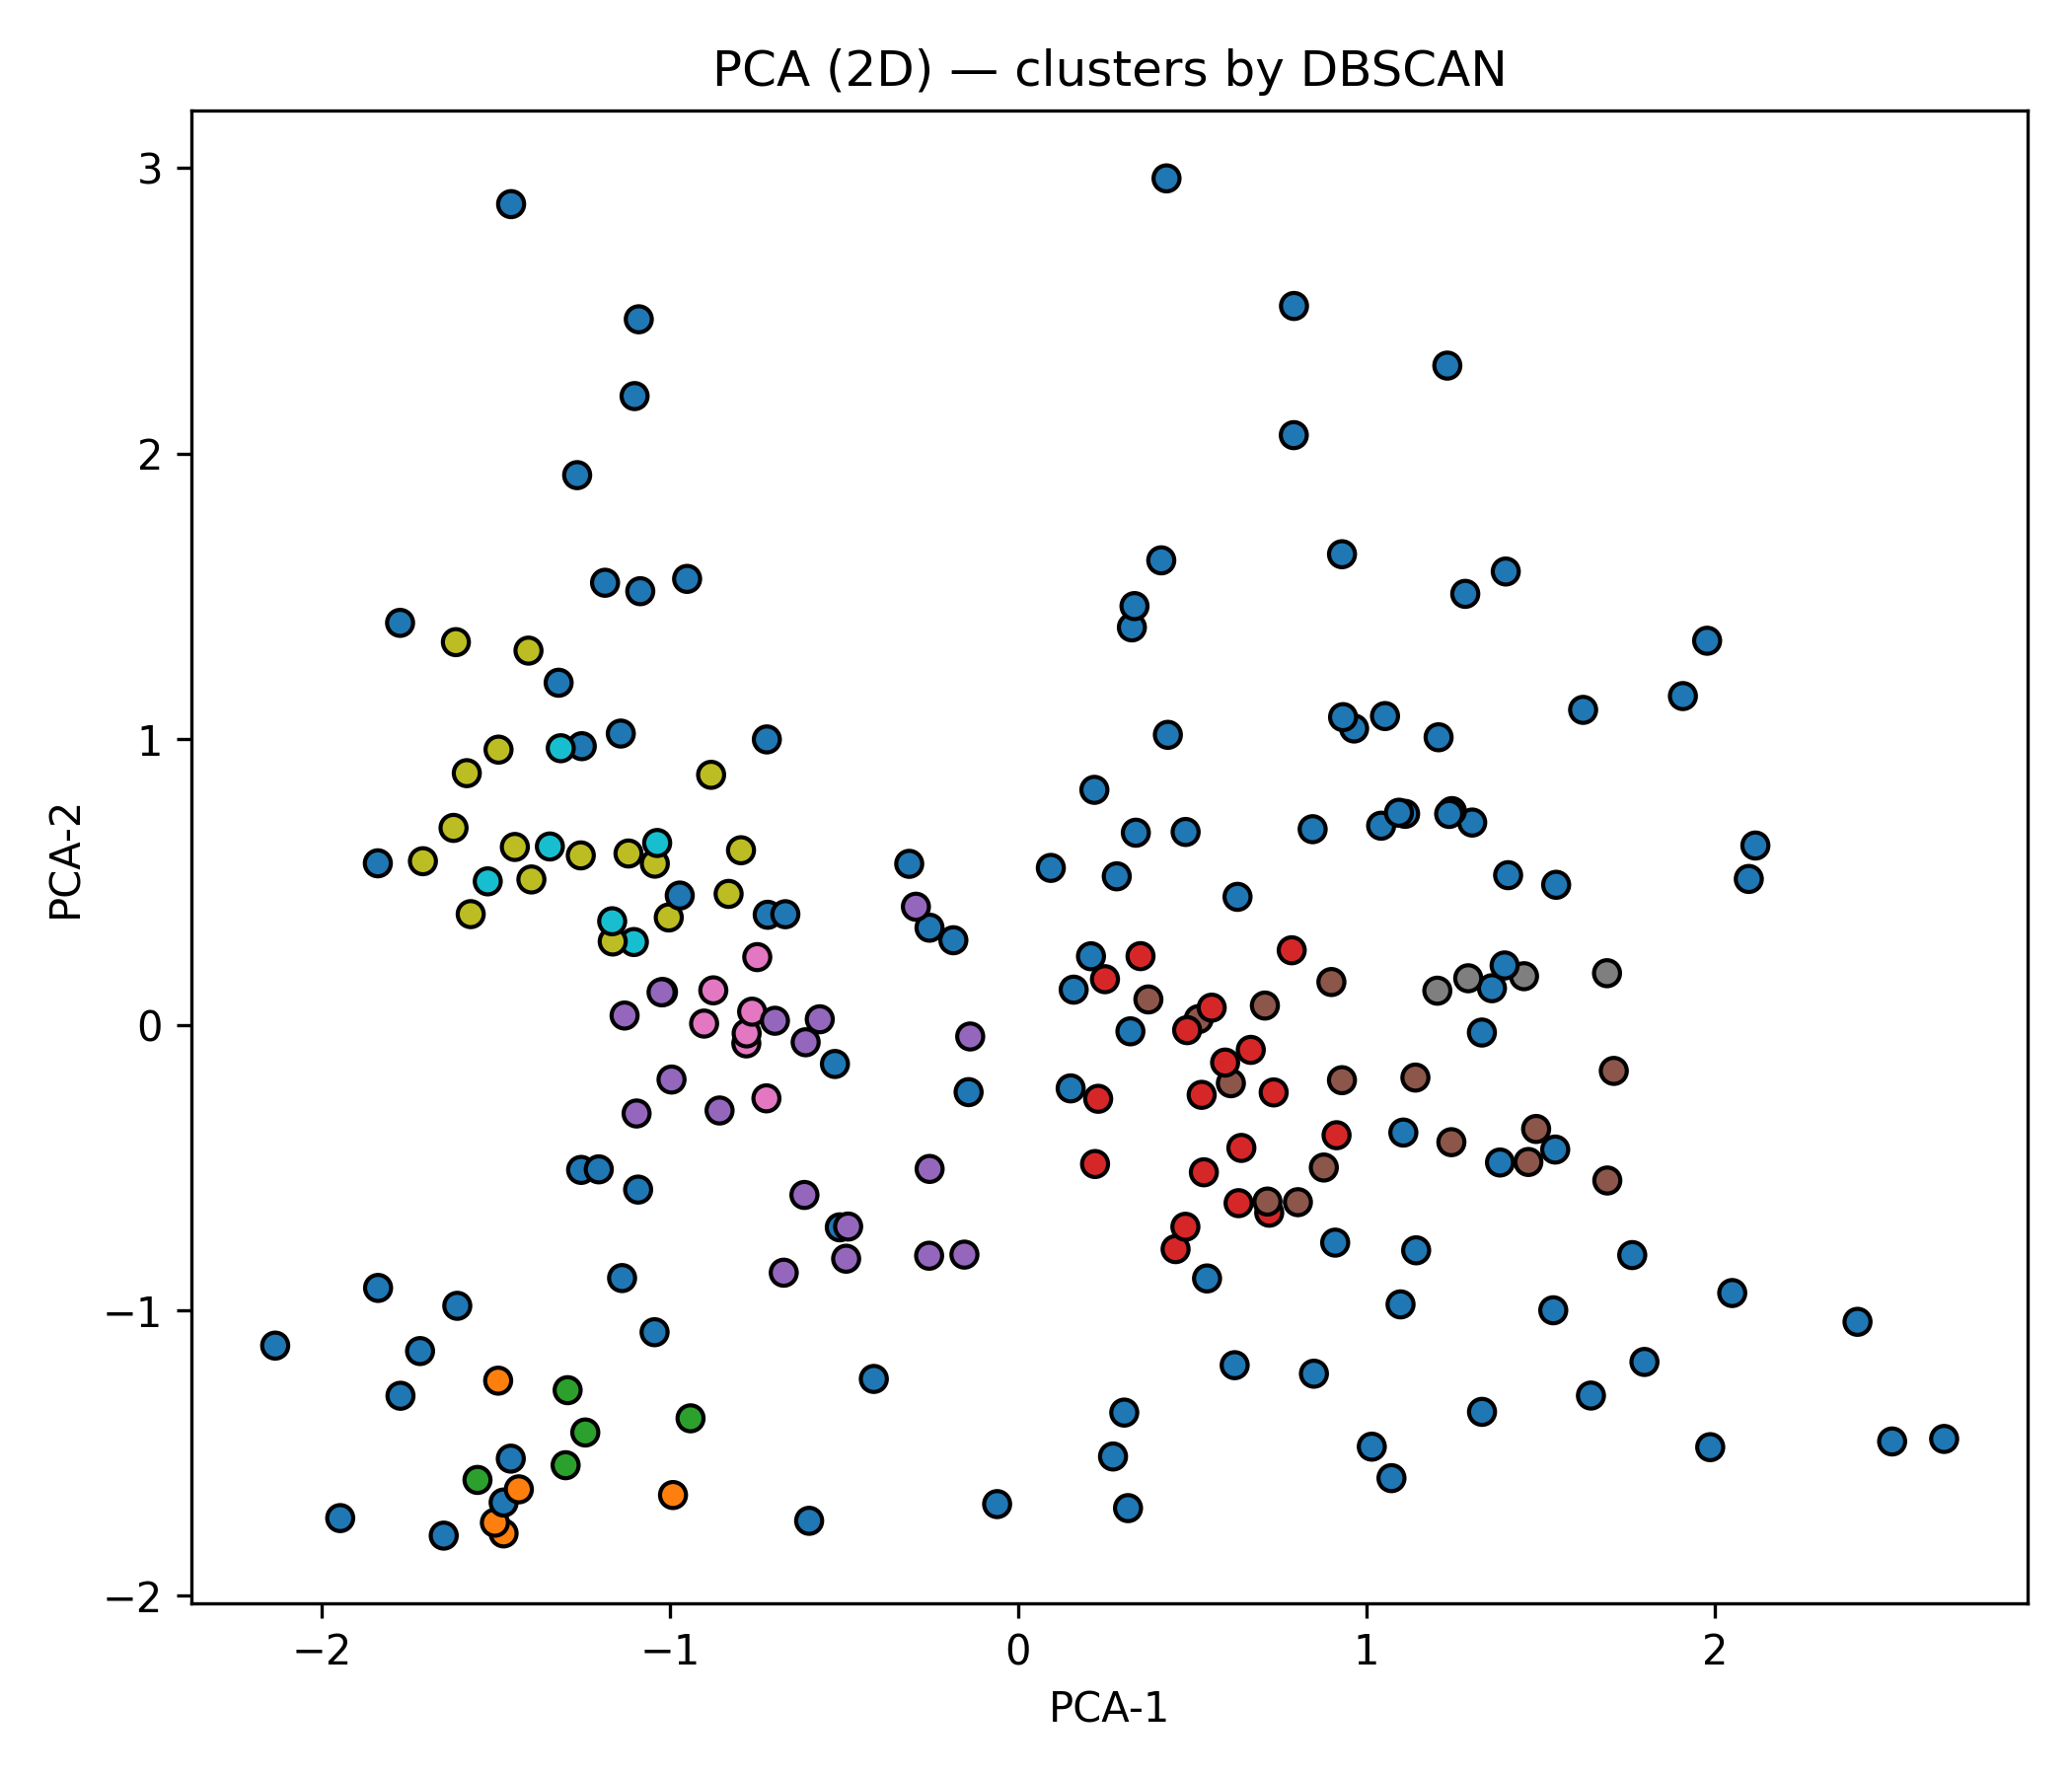
\includegraphics[width=0.3\linewidth]{figures2/pca_dbscan.png}}\\[0.6em]
    \subfloat[t-SNE--KMeans]{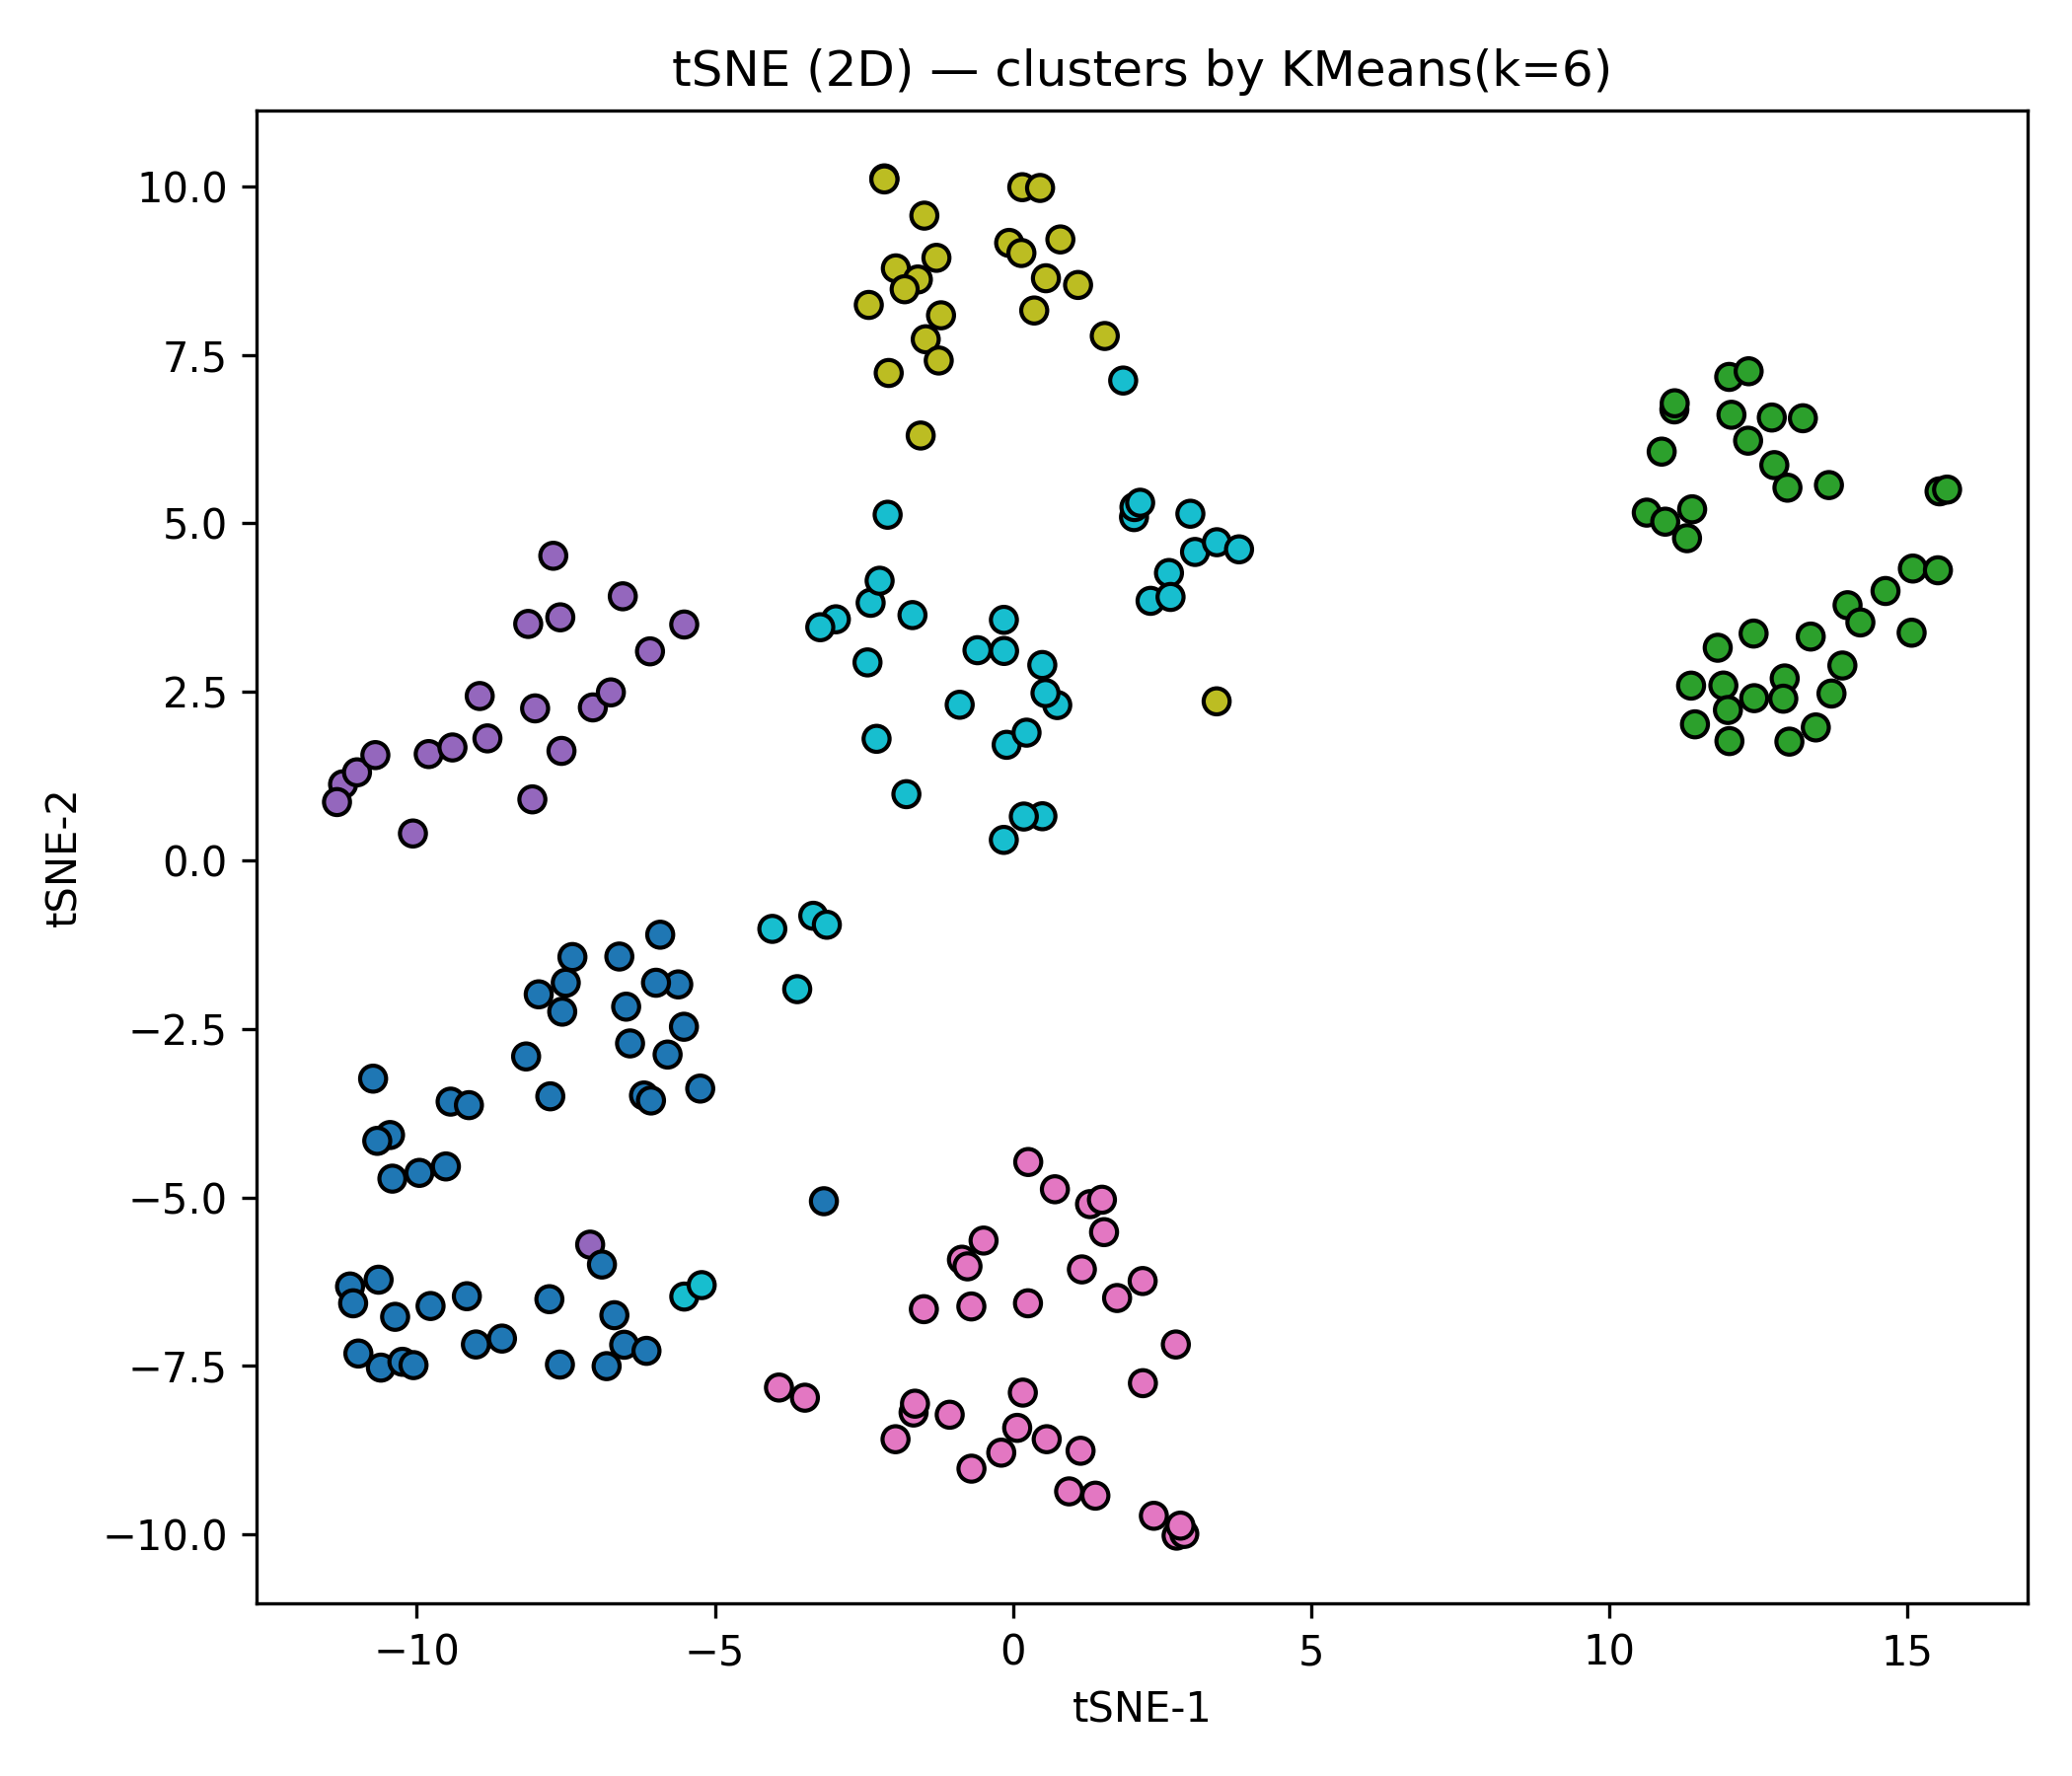
\includegraphics[width=0.3\linewidth]{figures2/tsne_kmeans.png}}
    \hfill
    \subfloat[t-SNE--Agglomerative]{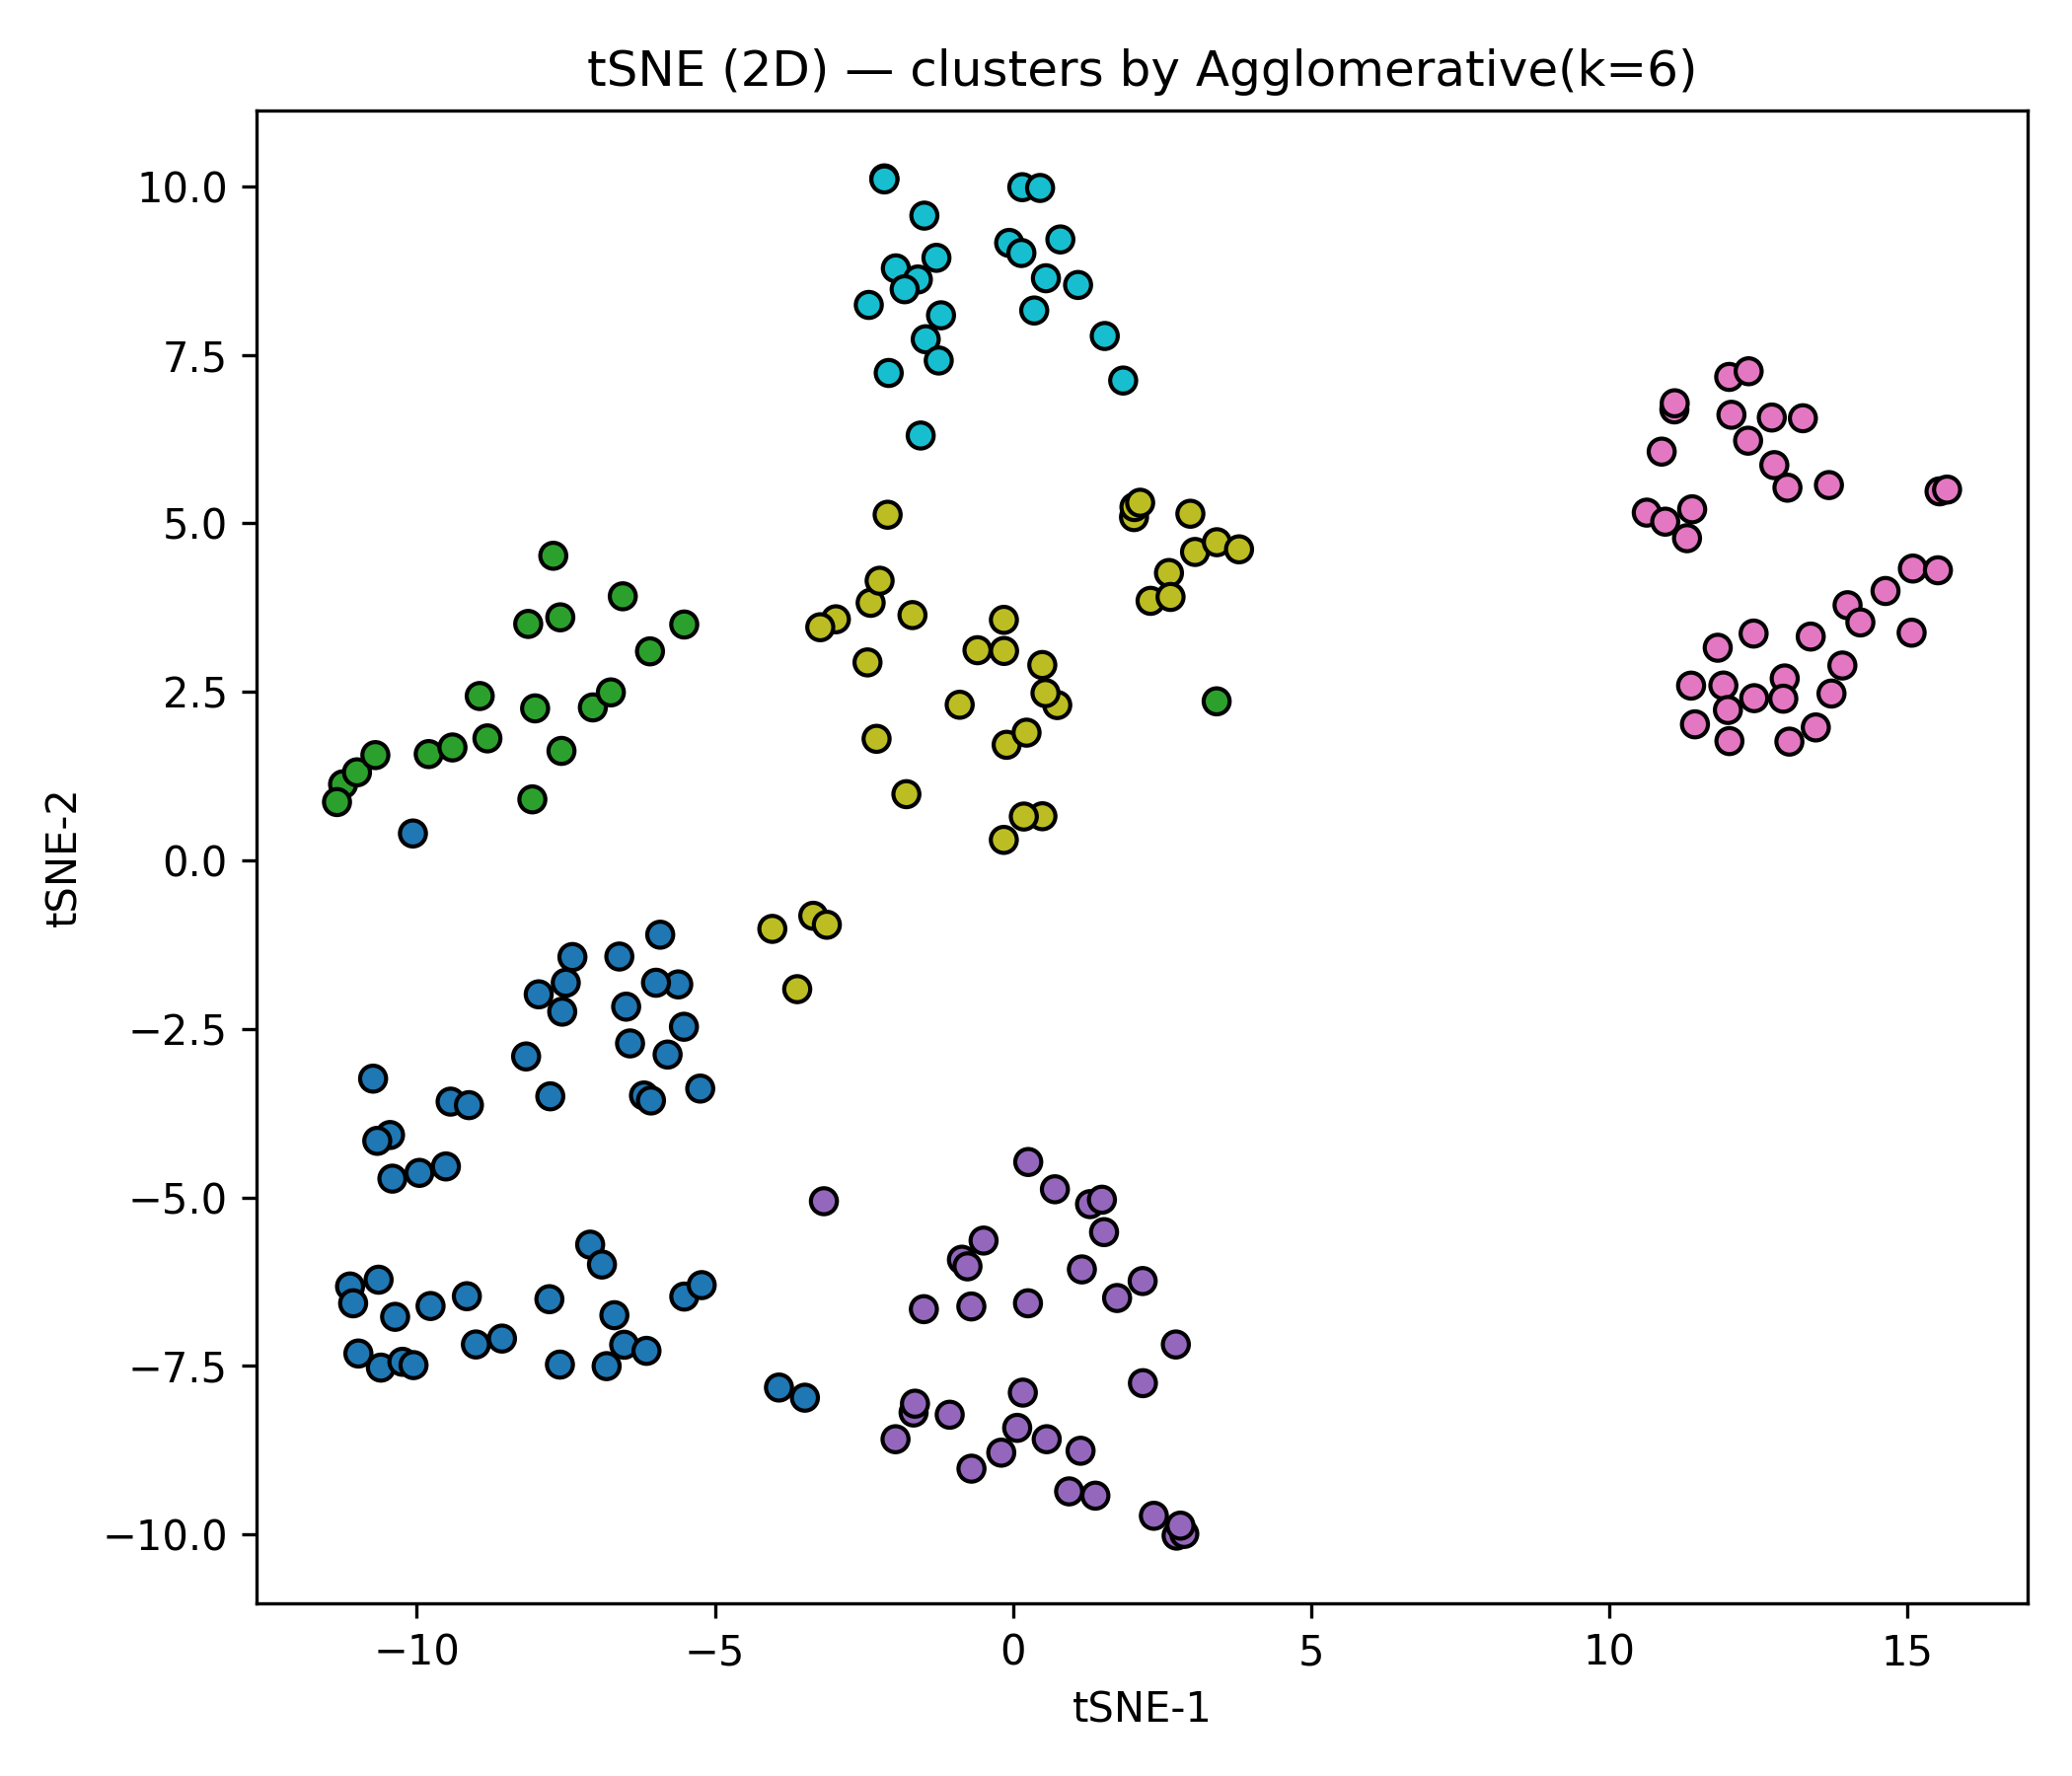
\includegraphics[width=0.3\linewidth]{figures2/tsne_agglomerative.png}}
    \hfill
    \subfloat[t-SNE--DBSCAN]{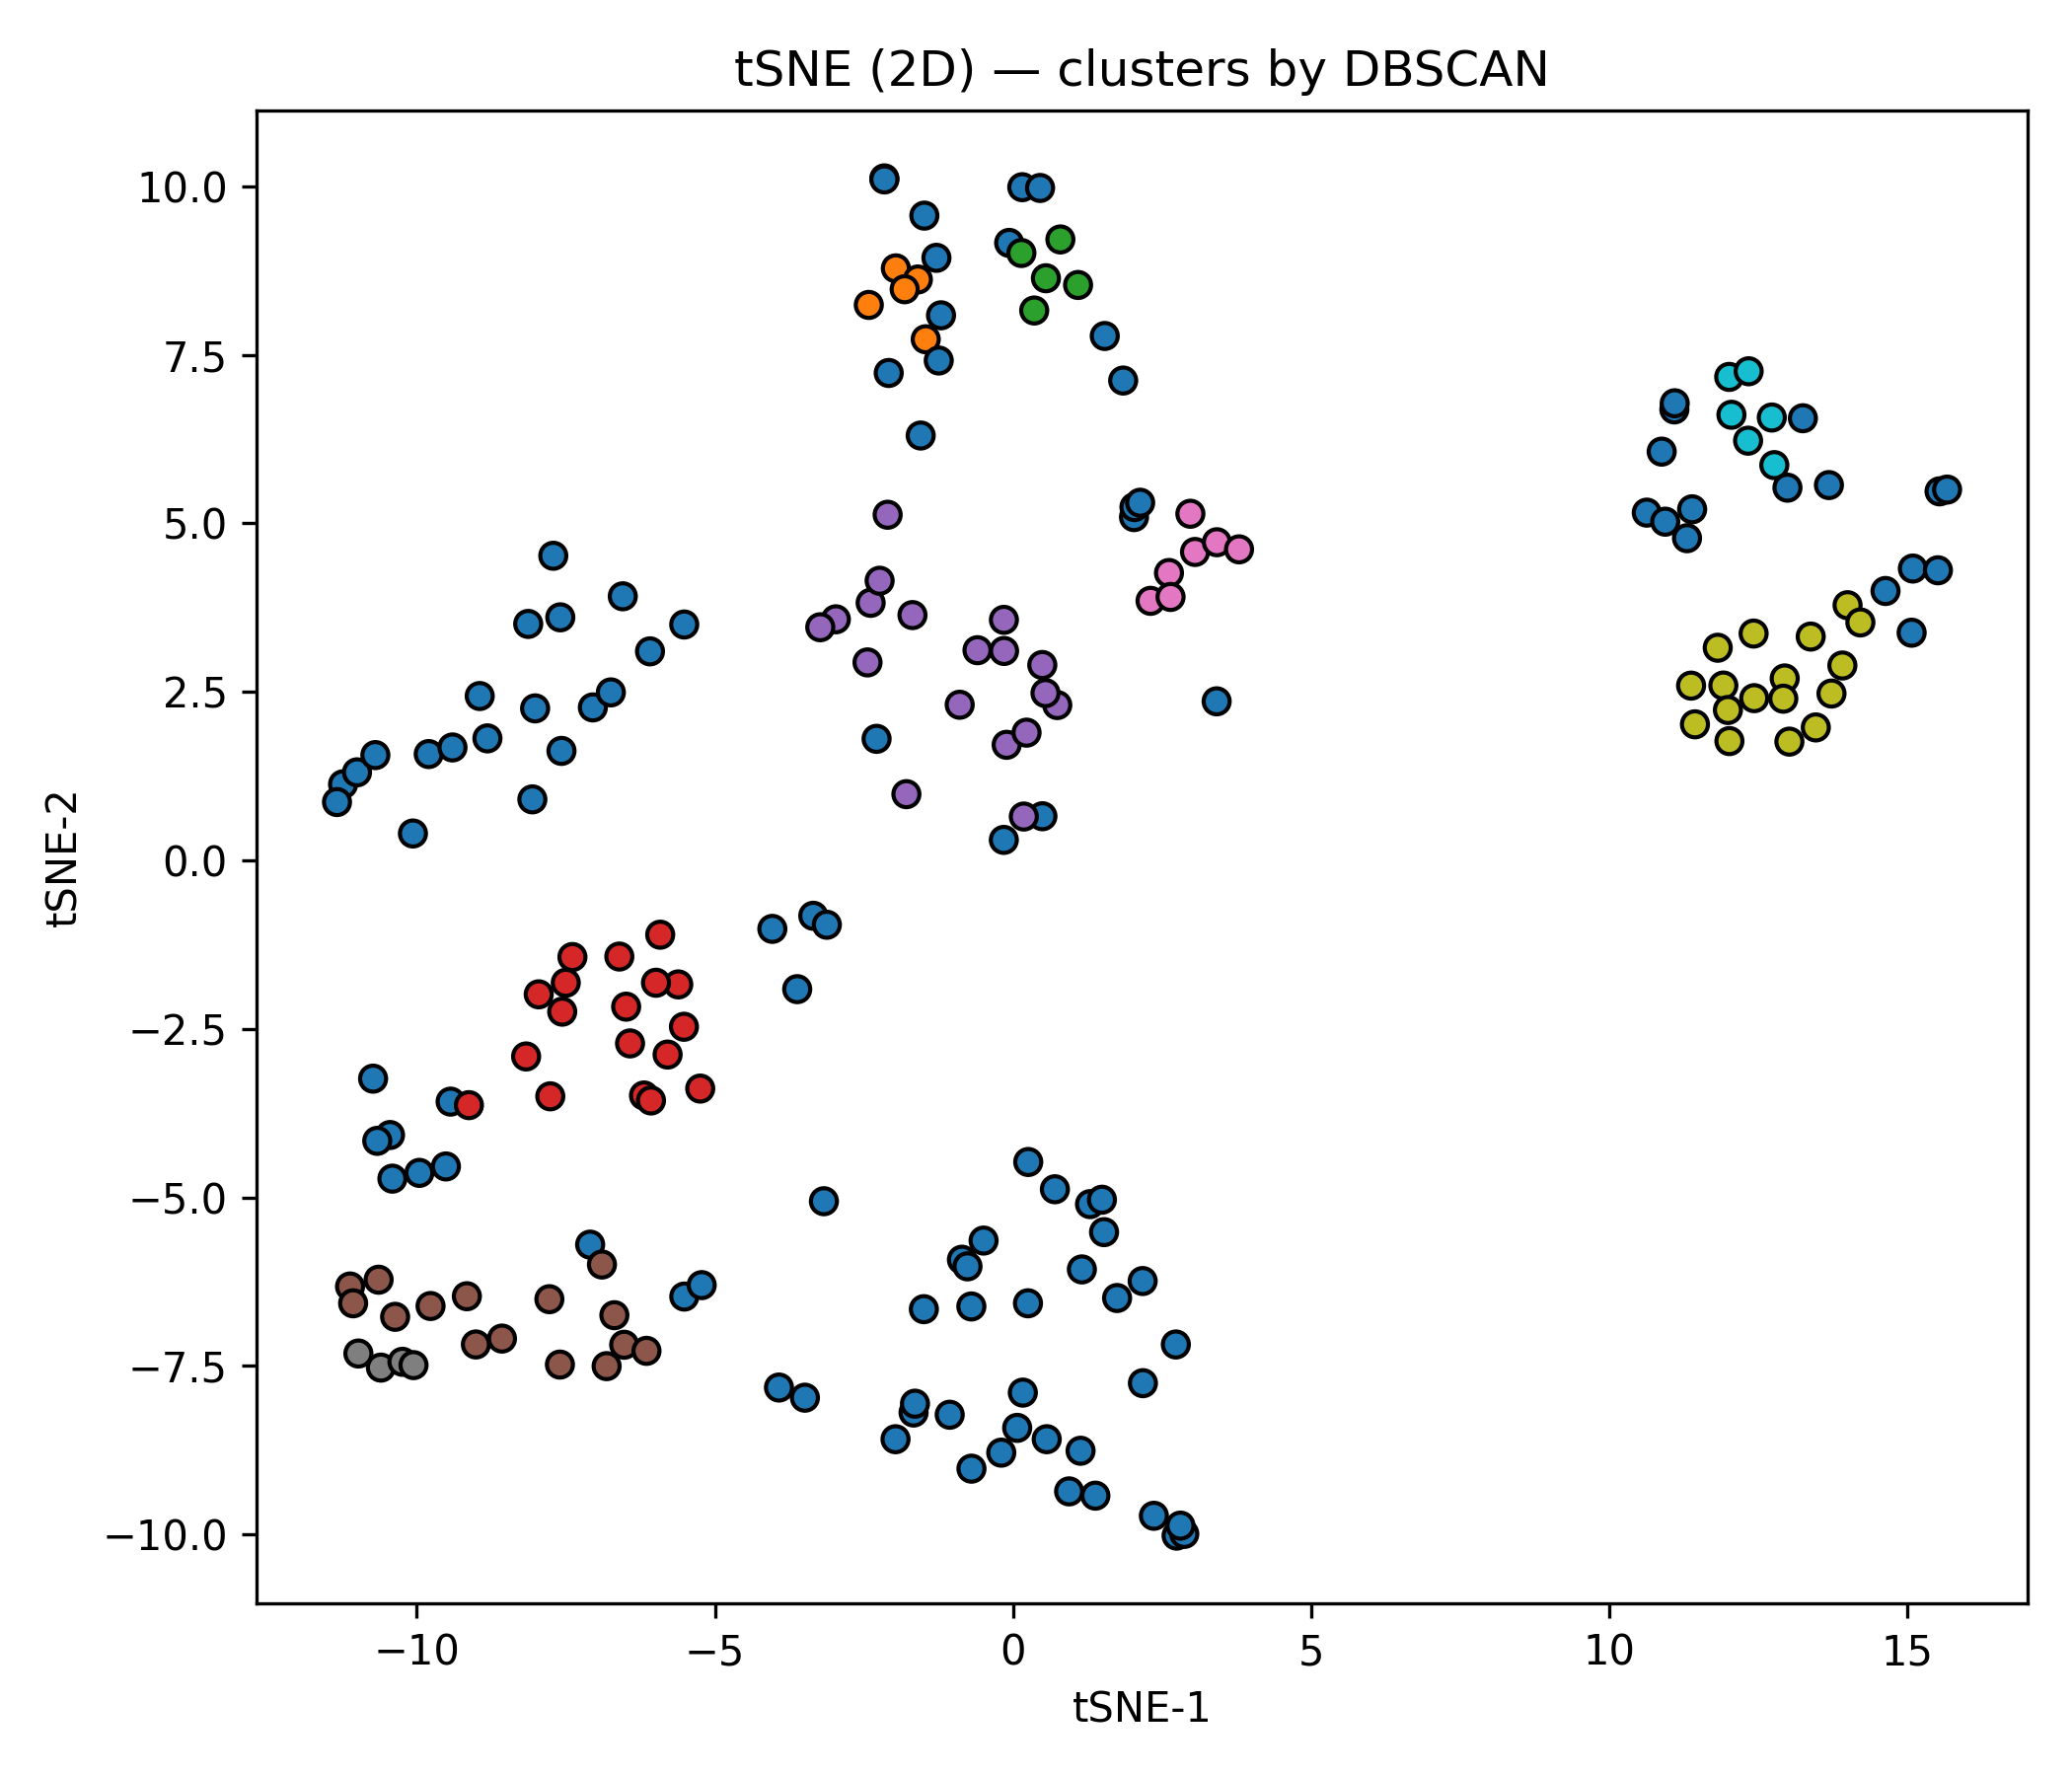
\includegraphics[width=0.3\linewidth]{figures2/tsne_dbscan.png}}
    \caption{二维降维后三种聚类算法的聚类结果(上:PCA;下:t-SNE)}
    \label{fig:pca_tsne_all}
\end{figure}

%----------------- 层次聚类树状图 -----------------
\begin{figure}[htbp]
    \centering
    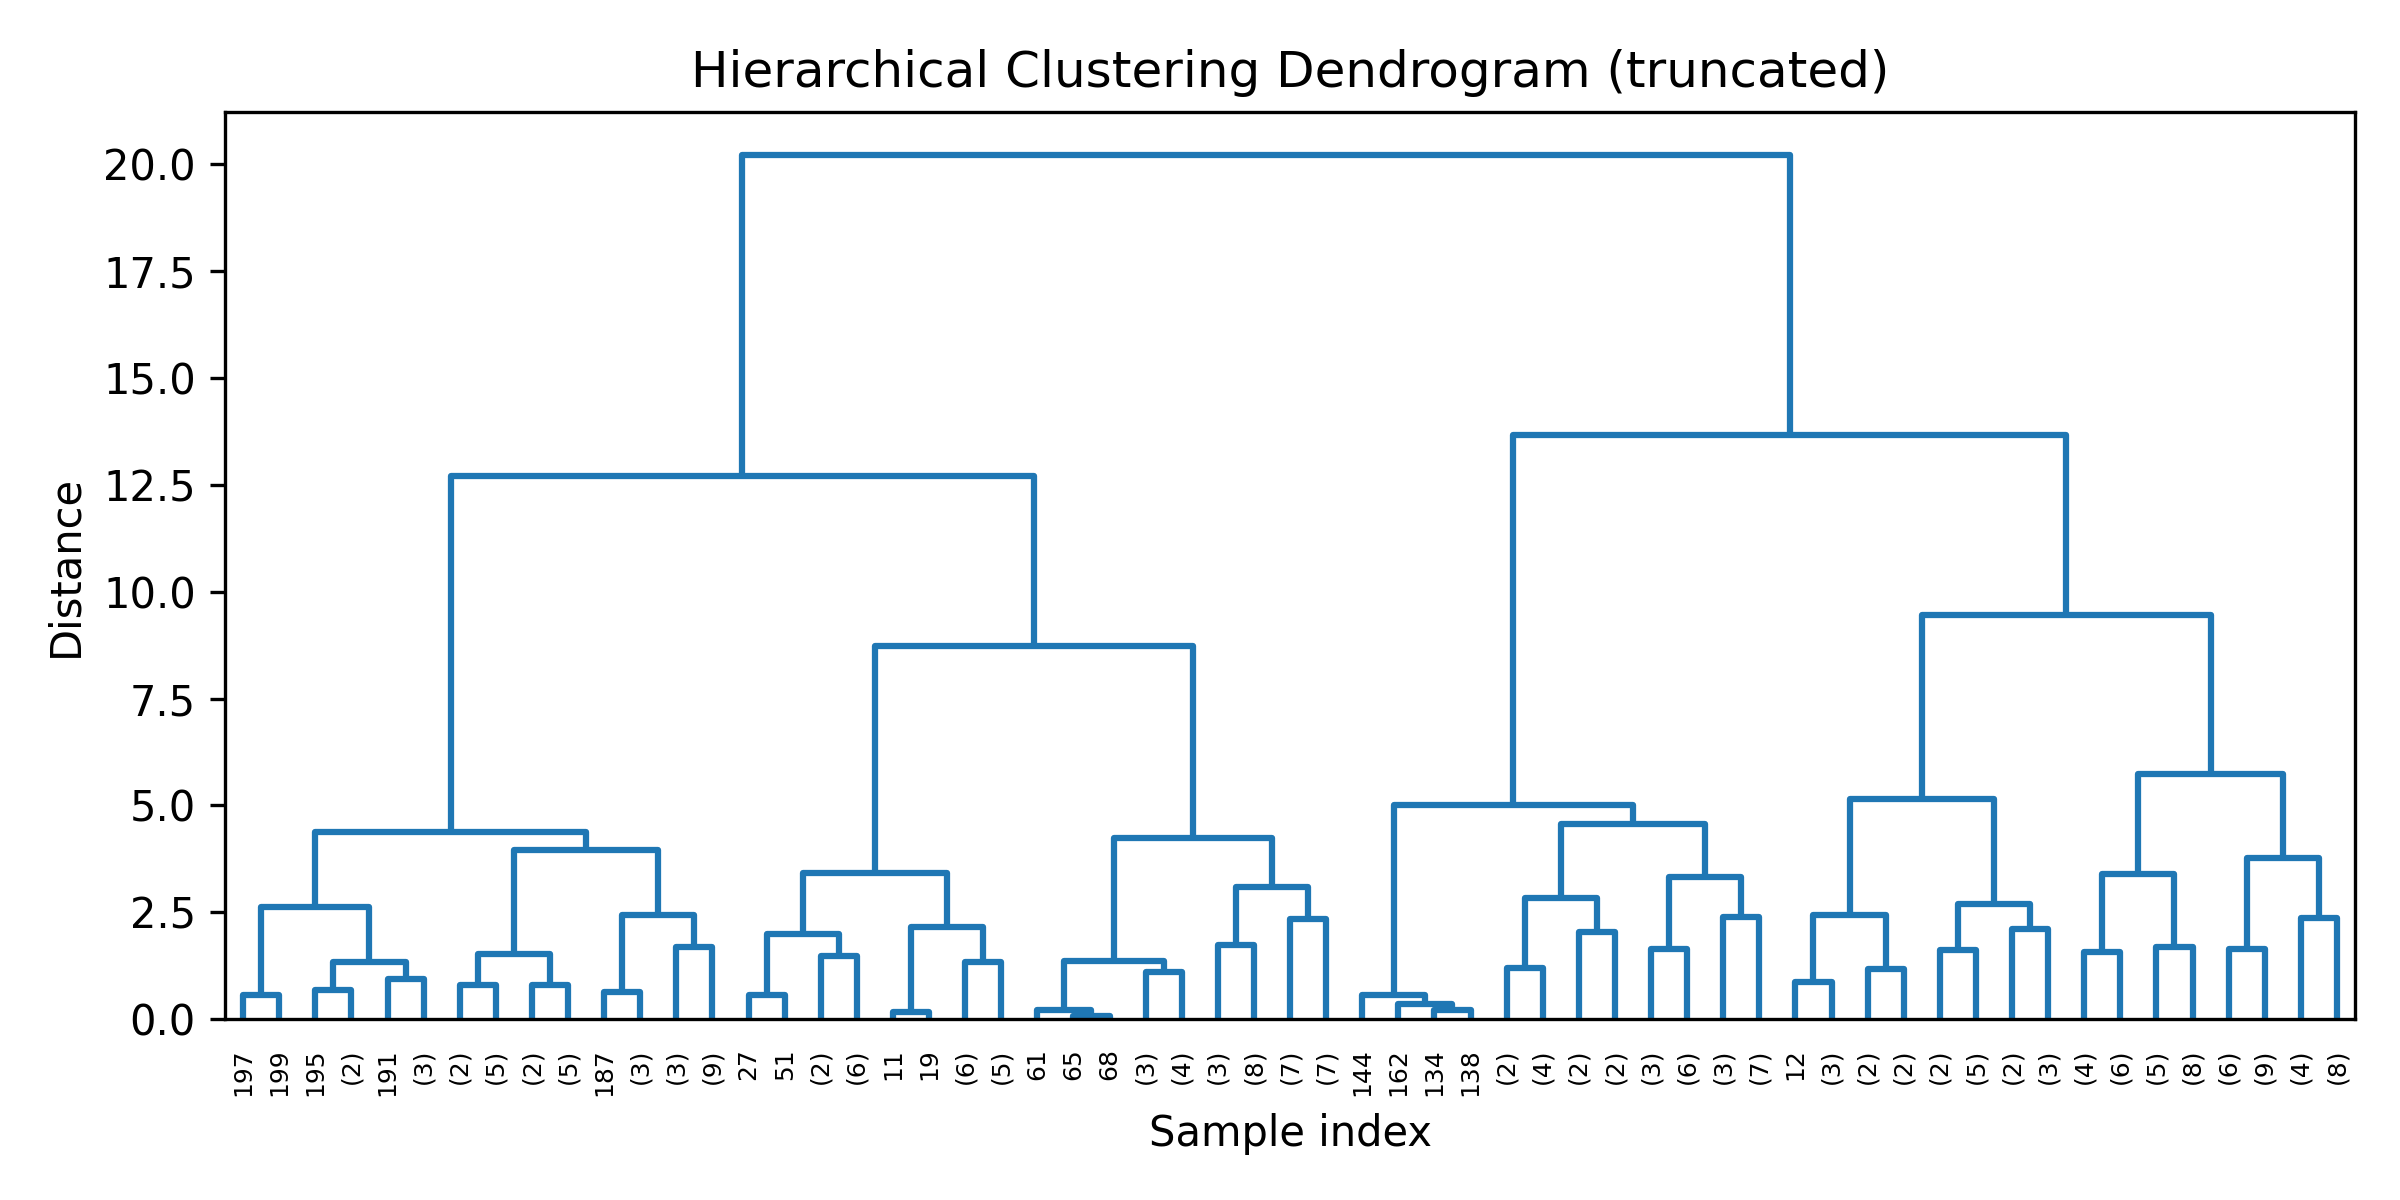
\includegraphics[width=\linewidth]{figures2/dendrogram.png}
    \caption{层次聚类的截断树状图(Ward linkage, level = 5)}
    \label{fig:dendrogram}
\end{figure}

%--------------------------------------------------
\paragraph{4.3 代码与文件结构}
\begin{itemize}
    \item 根目录含 \texttt{task1.py} 与 \texttt{task2.py},对应监督/无监督实验。
    \item 生成的图片分别保存于 \texttt{./figures} 与 \texttt{./figures2},脚本已自动创建文件夹。
    \item LaTeX 文档 \texttt{report.tex} 位于 \texttt{LAB2/},编译后生成 \texttt{report.pdf};所有图片使用相对路径引用。
\end{itemize}


\subsection*{4. 实现内容}

\paragraph{4.1 监督学习模块(\texttt{task1.py})}
\begin{enumerate}[label=\arabic*)]
    \item \textbf{数据载入与缺失值注入}\\
          读取原始 Iris 数据集后,以随机比例 \(\text{ratio}=0.1\) 将四个特征列注入缺失值,用于验证不同缺失值处理策略的鲁棒性。
    \item \textbf{缺失值处理策略}\\
          依次采用 \textit{drop}(直接删除含缺失样本)、\textit{mean}、\textit{median} 与 \textit{knn}(\(k=5\))四种策略,对训练集和测试集分别处理并保持标签一致性。
    \item \textbf{特征缩放}\\
          对填补/删除后的数据使用 \texttt{StandardScaler} 进行零均值、单位方差标准化。
    \item \textbf{模型训练与评估}\\
          选取 \textbf{Logistic Regression}、\textbf{Decision Tree}、\textbf{SVM (RBF)} 与 \textbf{\(k\)-NN} 四种经典分类器,分别在四种缺失值策略产生的数据集上训练。\par
          评估指标包括:\emph{Accuracy} 与 \emph{加权 \(F_1\)}。此外,针对每组 ``模型–策略'' 组合生成对应的混淆矩阵并保存。
    \item \textbf{结果可视化}\\[-0.8em]
          \begin{itemize}
              \item 比较柱状图:\verb|figures/accuracy_comparison.png| 与 \verb|figures/f1_comparison.png| (见图~\ref{fig:acc_f1_bar})。
              \item 混淆矩阵热力图:共 \(4 \times 4\) 张,命名为
                    \verb|figures/confmat_<strategy>_<model>.png|;本文仅示例其中两张(图~\ref{fig:confmat_drop_dt})。
          \end{itemize}
\end{enumerate}

% ---------- 监督学习核心算法 ----------
\begin{lstlisting}[language=Python, caption={核心算法实现:监督学习模块}]
# 1) 缺失值处理 + 标准化
def preprocess(X_train, X_test, strategy: str):
    """
    根据 strategy(drop/mean/median/knn) 处理缺失值并标准化
    返回处理后的 Xt, Xv
    """
    if strategy == "drop":
        mask_tr = ~np.isnan(X_train).any(axis=1)
        mask_te = ~np.isnan(X_test).any(axis=1)
        return X_train[mask_tr], X_test[mask_te]

    if strategy == "mean":
        imp = SimpleImputer(strategy="mean")
    elif strategy == "median":
        imp = SimpleImputer(strategy="median")
    elif strategy == "knn":
        imp = KNNImputer(n_neighbors=5)
    else:
        raise ValueError(f"Unknown strategy: {strategy}")

    scaler = StandardScaler()
    Xt = scaler.fit_transform(imp.fit_transform(X_train))
    Xv = scaler.transform(imp.transform(X_test))
    return Xt, Xv


# 2) 单模型评估(返回 accuracy 与 weighted-F1)
def evaluate_one(clf, Xt, yt, Xv, yv):
    clf.fit(Xt, yt)
    pred = clf.predict(Xv)
    return {
        "acc": accuracy_score(yv, pred),
        "f1":  f1_score(yv, pred, average="weighted"),
    }
\end{lstlisting}

% ---------- 无监督学习核心算法 ----------
\begin{lstlisting}[language=Python, caption={核心算法实现:无监督学习模块}]
def elbow_and_silhouette(X, k_max: int = 10) -> int:
    """
    计算 2..k_max 的惯性与 Silhouette;按 Silhouette 最大化选 k*
    """
    inertias, sils = [], []
    for k in range(2, k_max + 1):
        km = KMeans(n_clusters=k, random_state=42).fit(X)
        inertias.append(km.inertia_)
        sils.append(silhouette_score(X, km.labels_))
    return int(np.argmax(sils)) + 2   # best k


def cluster_and_metrics(X, k_opt: int) -> dict[str, dict[str, float]]:
    """
    在最优簇数 k_opt 下比较三种聚类算法并计算内部指标
    返回形如 {"KMeans": {"sil":..,"CH":..,"DB":..}, ...}
    """
    algos = {
        "KMeans": KMeans(n_clusters=k_opt, random_state=42),
        "Agglomerative": AgglomerativeClustering(n_clusters=k_opt),
        "DBSCAN": DBSCAN(eps=0.5, min_samples=5),
    }
    metrics = {}
    for name, algo in algos.items():
        labels = algo.fit_predict(X)
        valid = (len(set(labels)) > 1) and not (len(set(labels)) == 2 and -1 in labels)
        metrics[name] = {
            "sil": silhouette_score(X, labels) if valid else float("nan"),
            "CH":  calinski_harabasz_score(X, labels),
            "DB":  davies_bouldin_score(X, labels),
        }
    return metrics
\end{lstlisting}


\begin{figure}[htbp]
    \centering
    \subfloat[Accuracy]{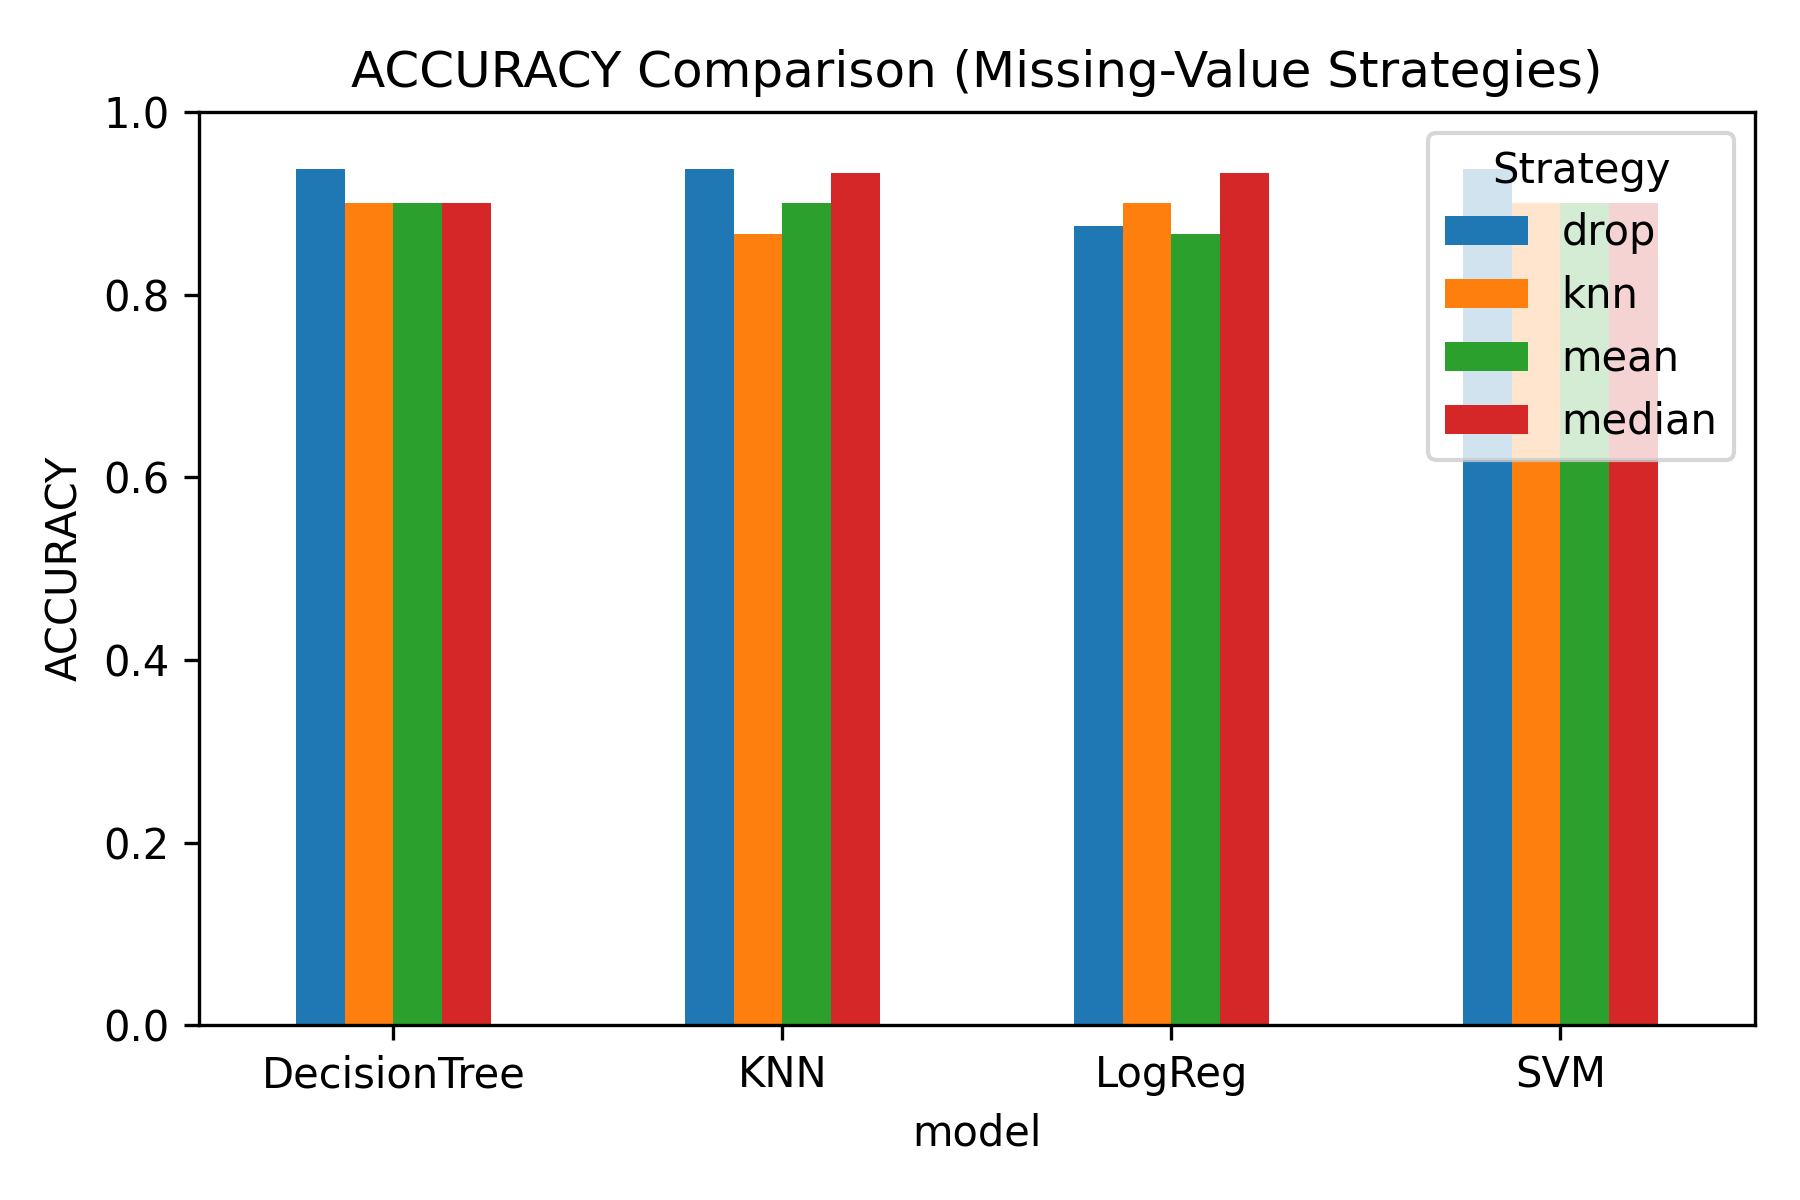
\includegraphics[width=0.48\linewidth]{figures/accuracy_comparison.png}}
    \hfill
    \subfloat[Weighted \( F_1 \)]{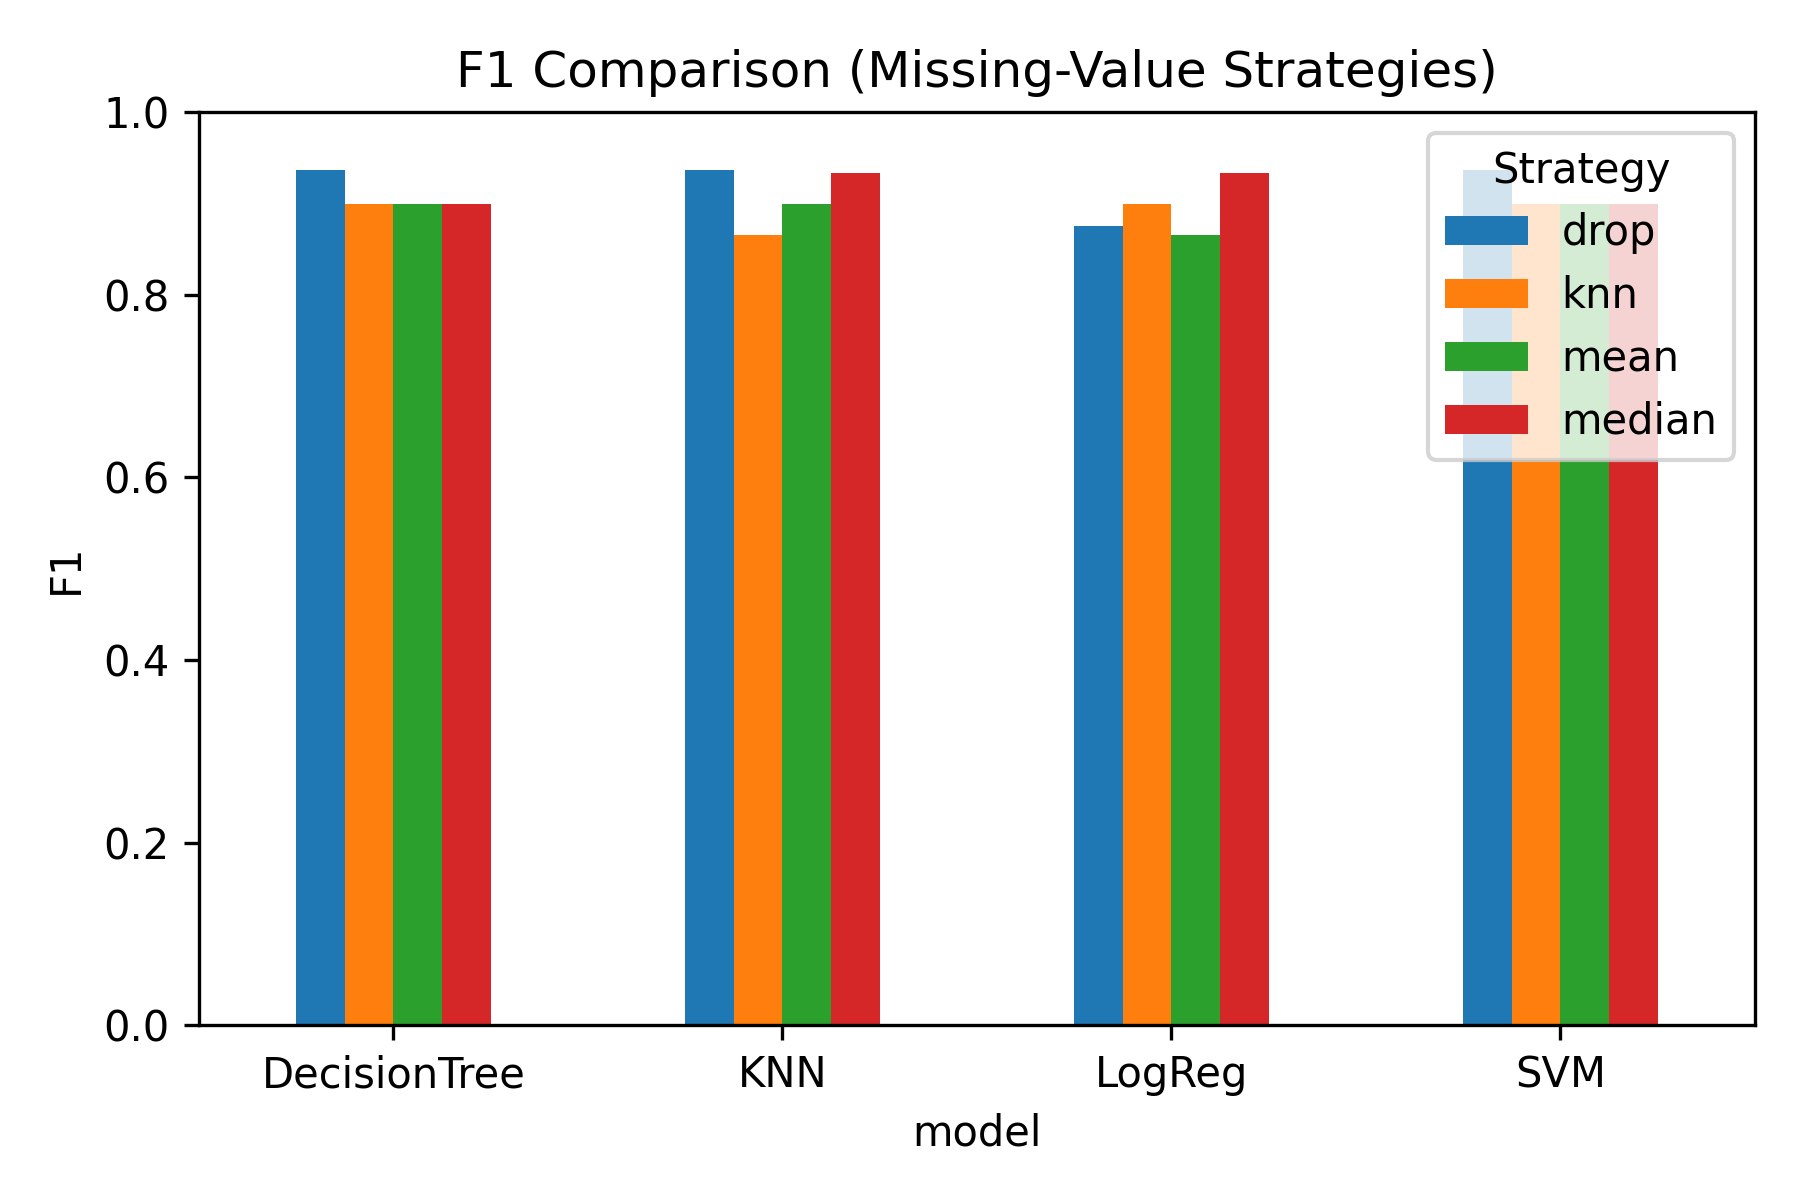
\includegraphics[width=0.48\linewidth]{figures/f1_comparison.png}}
    \caption{不同缺失值处理策略下四类模型的总体性能比较}
    \label{fig:acc_f1_bar}
\end{figure}

\begin{figure}[htbp]
    \centering
    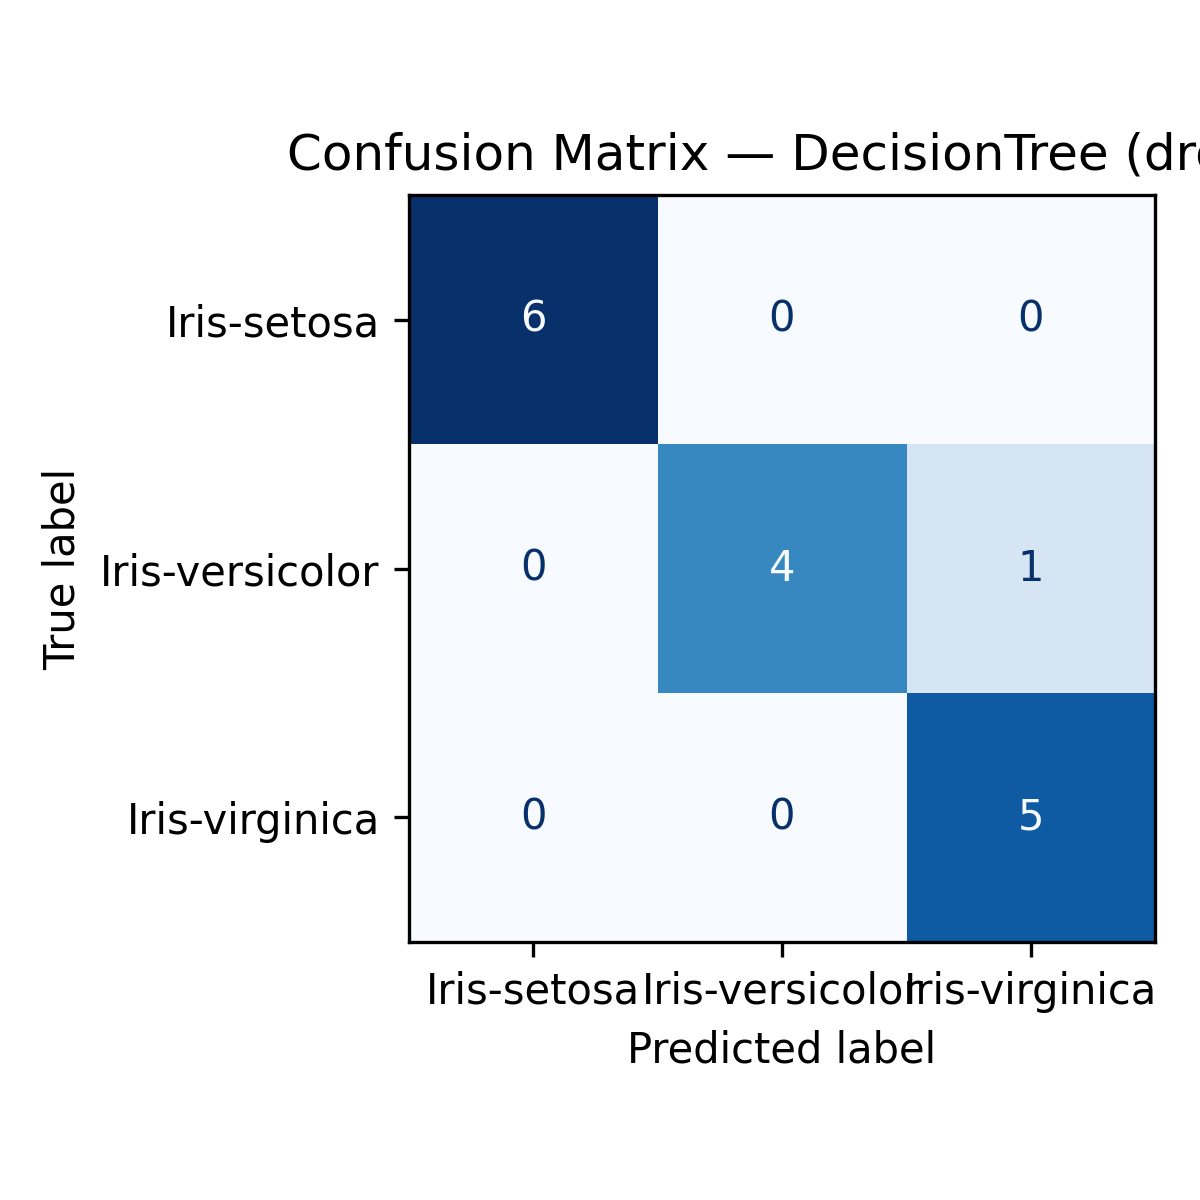
\includegraphics[width=0.48\linewidth]{figures/confmat_drop_DecisionTree.png}
    \caption{示例——\textit{drop} 策略下 Decision Tree 的混淆矩阵}
    \label{fig:confmat_drop_dt}
\end{figure}

\paragraph{4.2 无监督学习模块(\texttt{task2.py})}
\begin{enumerate}[label=\arabic*)]
    \item \textbf{数据清洗与预处理}\\
          载入 \textit{Mall Customers} 数据集,先对 ``Age''、``AnnualIncome''、``SpendingScore'' 采取三倍 IQR Winsorization 去除极端离群点,再统一标准化;性别列经 Label Encoding,最终特征维数为 \(4\)。
    \item \textbf{降维可视化}\\
          使用 \textbf{PCA} 及 \textbf{t-SNE} 将特征映射到二维平面(图~\ref{fig:pca_tsne_km})。
    \item \textbf{最优簇数确定}\\
          对 \(k=2\!:\!10\) 的 K-Means 计算惯性与轮廓系数,绘制 \emph{Elbow} 与 \emph{Silhouette} 曲线(图~\ref{fig:elbow_silhouette}),选取轮廓系数最大时的 \(k^\ast=6\)。
    \item \textbf{聚类算法比较}\\
          在 \(k^\ast\) 下运行
          \textbf{K-Means}、\textbf{Agglomerative} 与 \textbf{DBSCAN},
          记录 \emph{Silhouette}、\emph{Calinski–Harabasz (CH)} 与 \emph{Davies–Bouldin (DB)} 三指标(代码中自动打印;K-Means 最优)。
    \item \textbf{结果可视化}\\[-0.8em]
          \begin{itemize}
              \item 聚类散点图:\verb|figures2/pca_kmeans.png|、\verb|figures2/tsne_kmeans.png| 等(图~\ref{fig:pca_tsne_km})。
              \item 层次聚类树状图:\verb|figures2/dendrogram.png|(图~\ref{fig:dendro})。
              \item 特征分布直方图与 ``Annual Income–Spending Score'' 散点图,见 \verb|figures2/feature_hist.png| 与 \verb|figures2/income_vs_score.png|。
          \end{itemize}
\end{enumerate}

\begin{figure}[htbp]
    \centering
    \subfloat[Elbow]{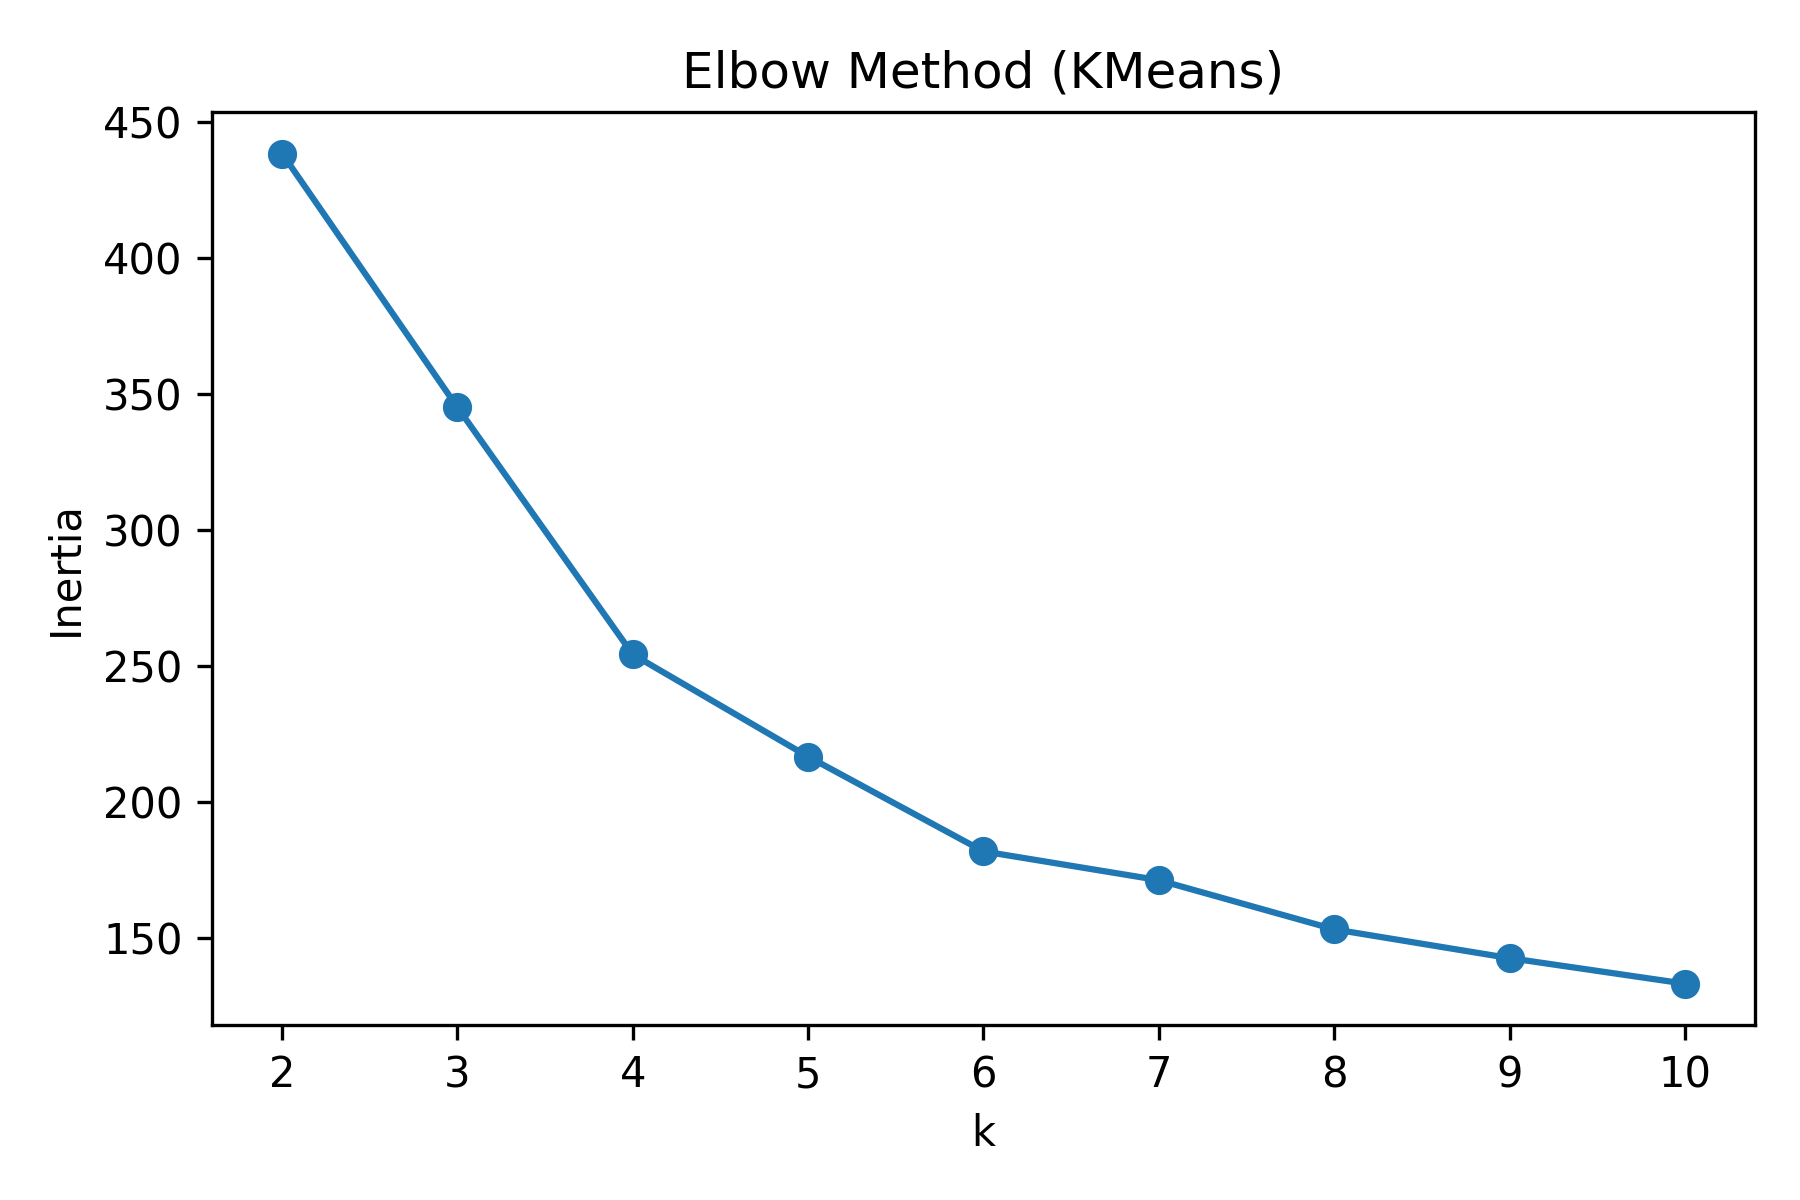
\includegraphics[width=0.48\linewidth]{figures2/elbow.png}}
    \hfill
    \subfloat[Silhouette]{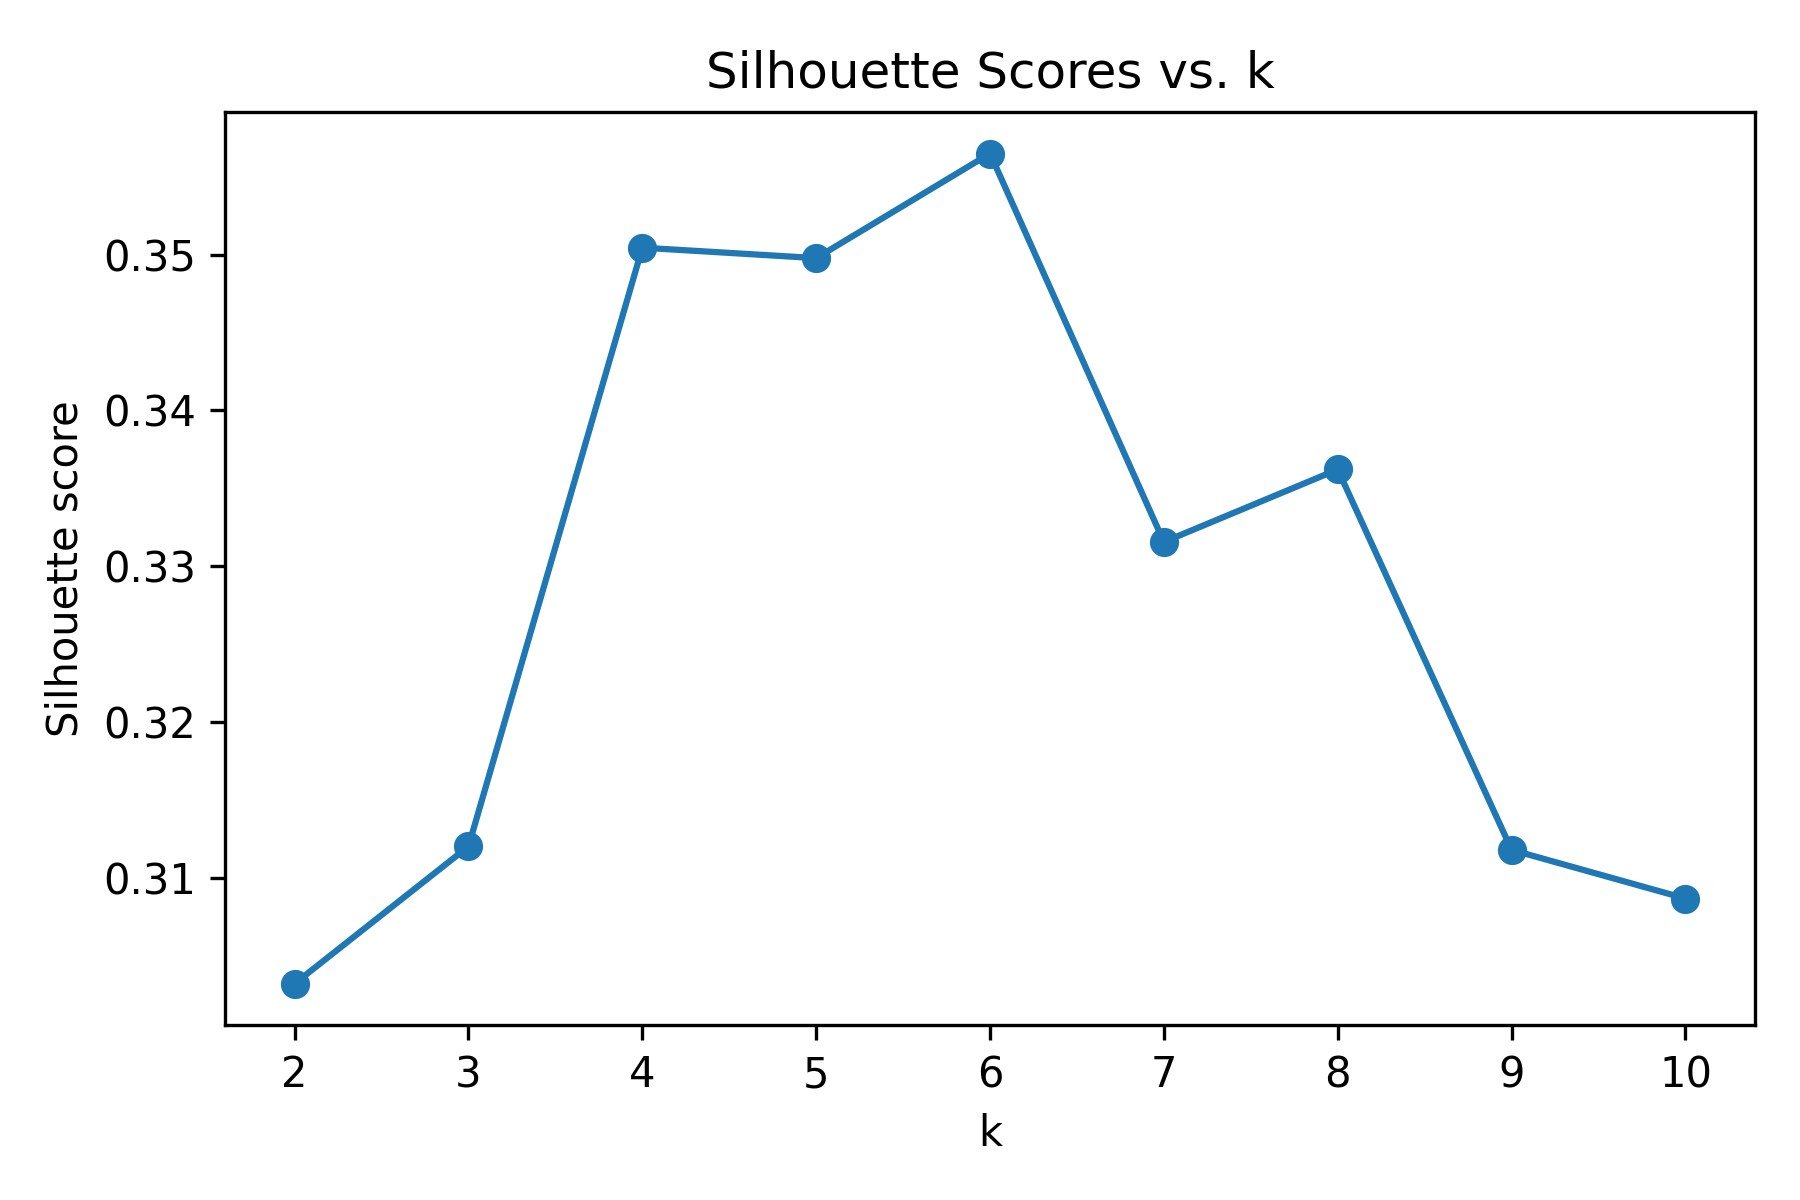
\includegraphics[width=0.48\linewidth]{figures2/silhouette_curve.png}}
    \caption{K-Means 不同 \(k\) 下的惯性与轮廓系数}
    \label{fig:elbow_silhouette}
\end{figure}

\begin{figure}[htbp]
    \centering
    \subfloat[PCA–KMeans]{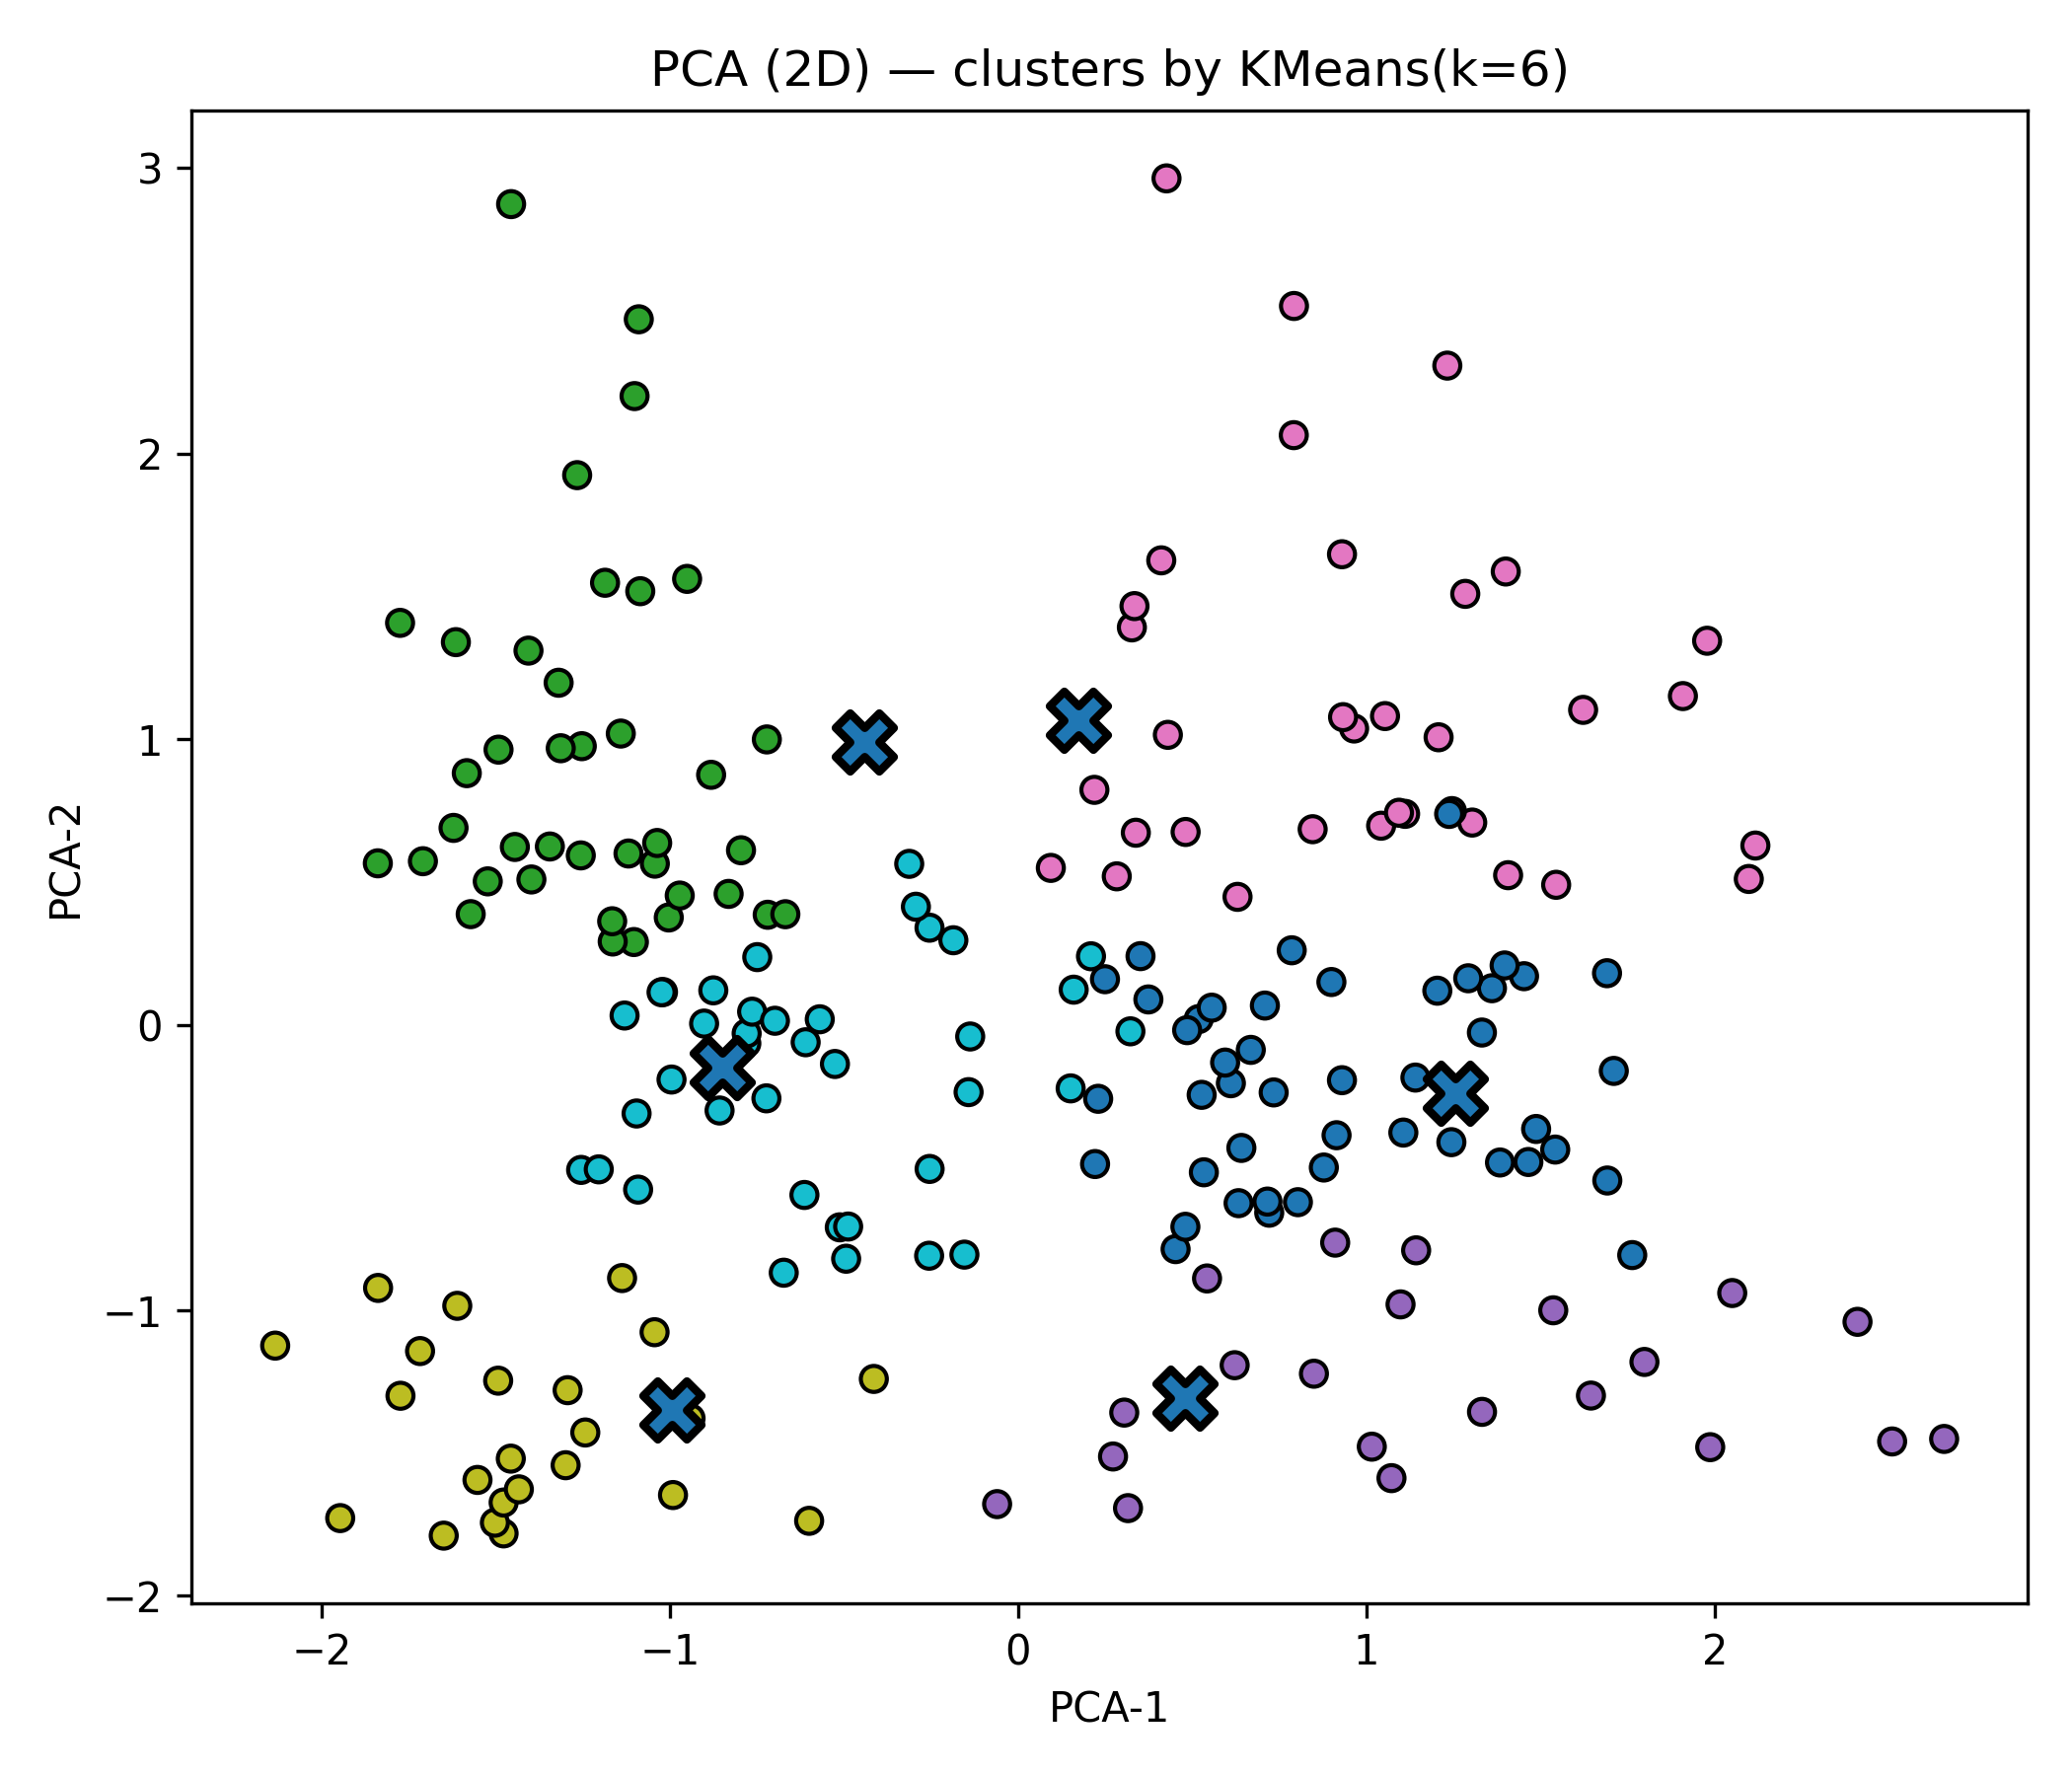
\includegraphics[width=0.48\linewidth]{figures2/pca_kmeans.png}}
    \hfill
    \subfloat[t-SNE–KMeans]{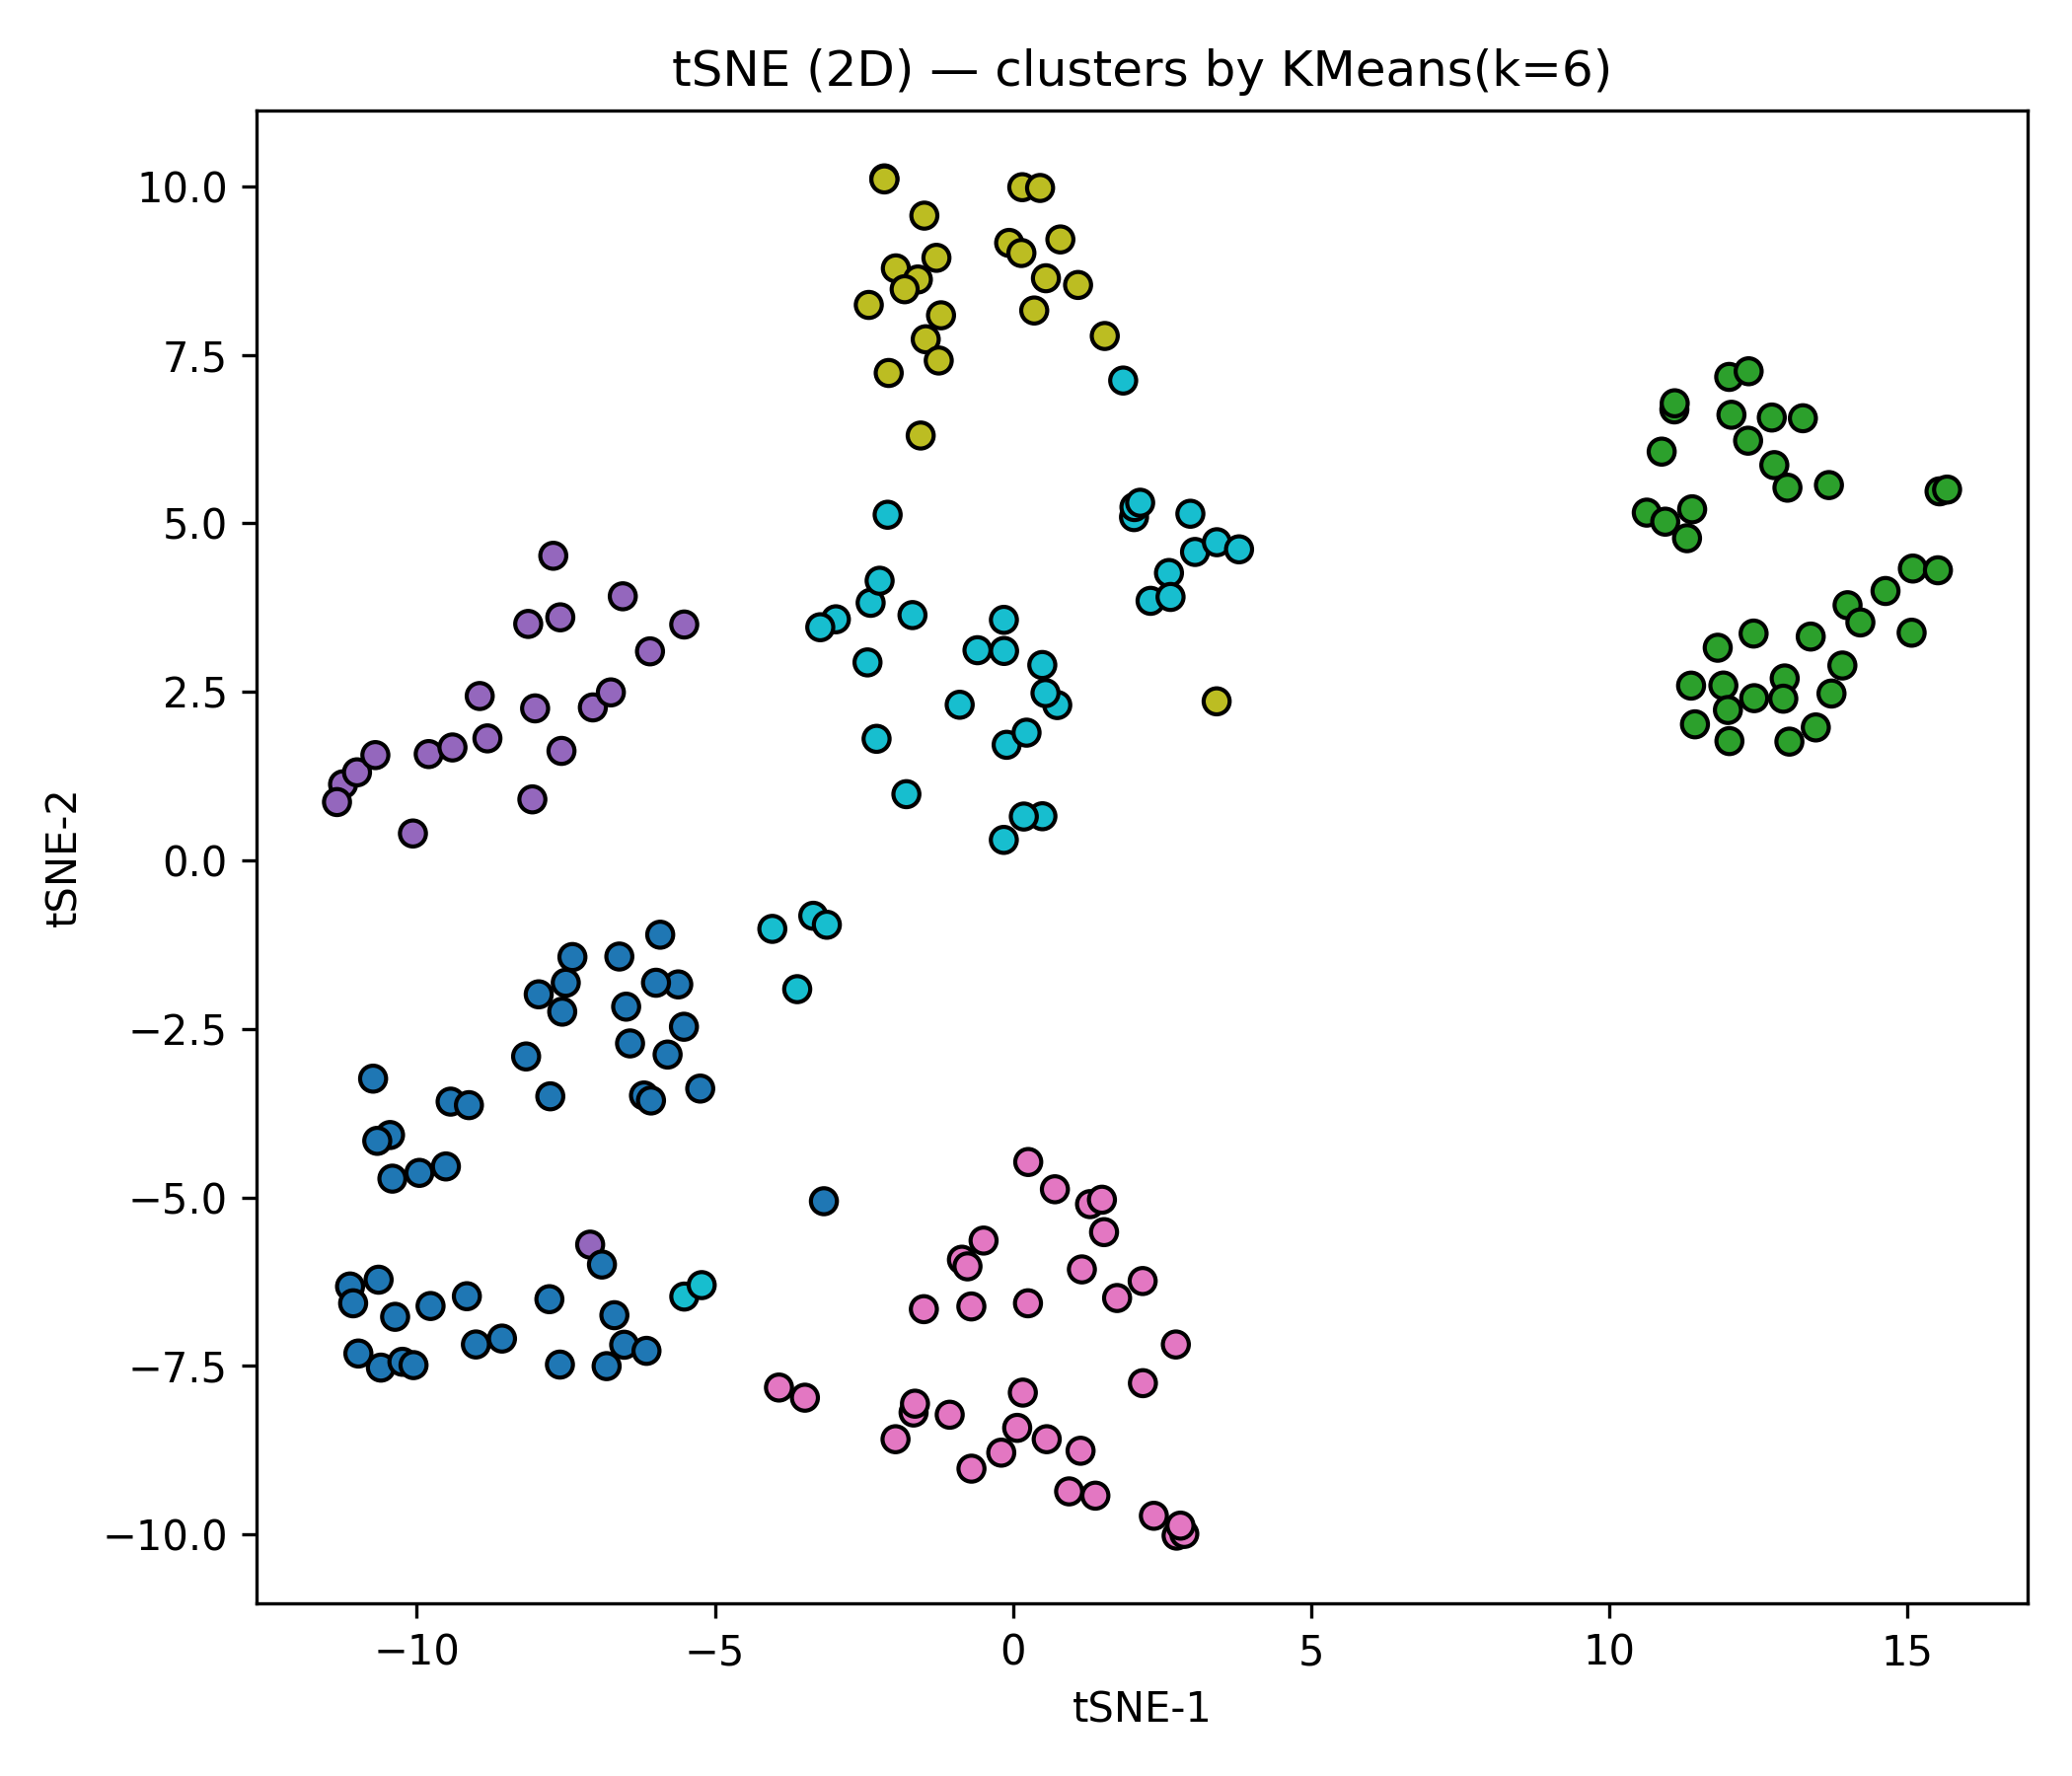
\includegraphics[width=0.48\linewidth]{figures2/tsne_kmeans.png}}
    \caption{二维降维后 K-Means (\(k=6\)) 聚类结果}
    \label{fig:pca_tsne_km}
\end{figure}

\begin{figure}[htbp]
    \centering
    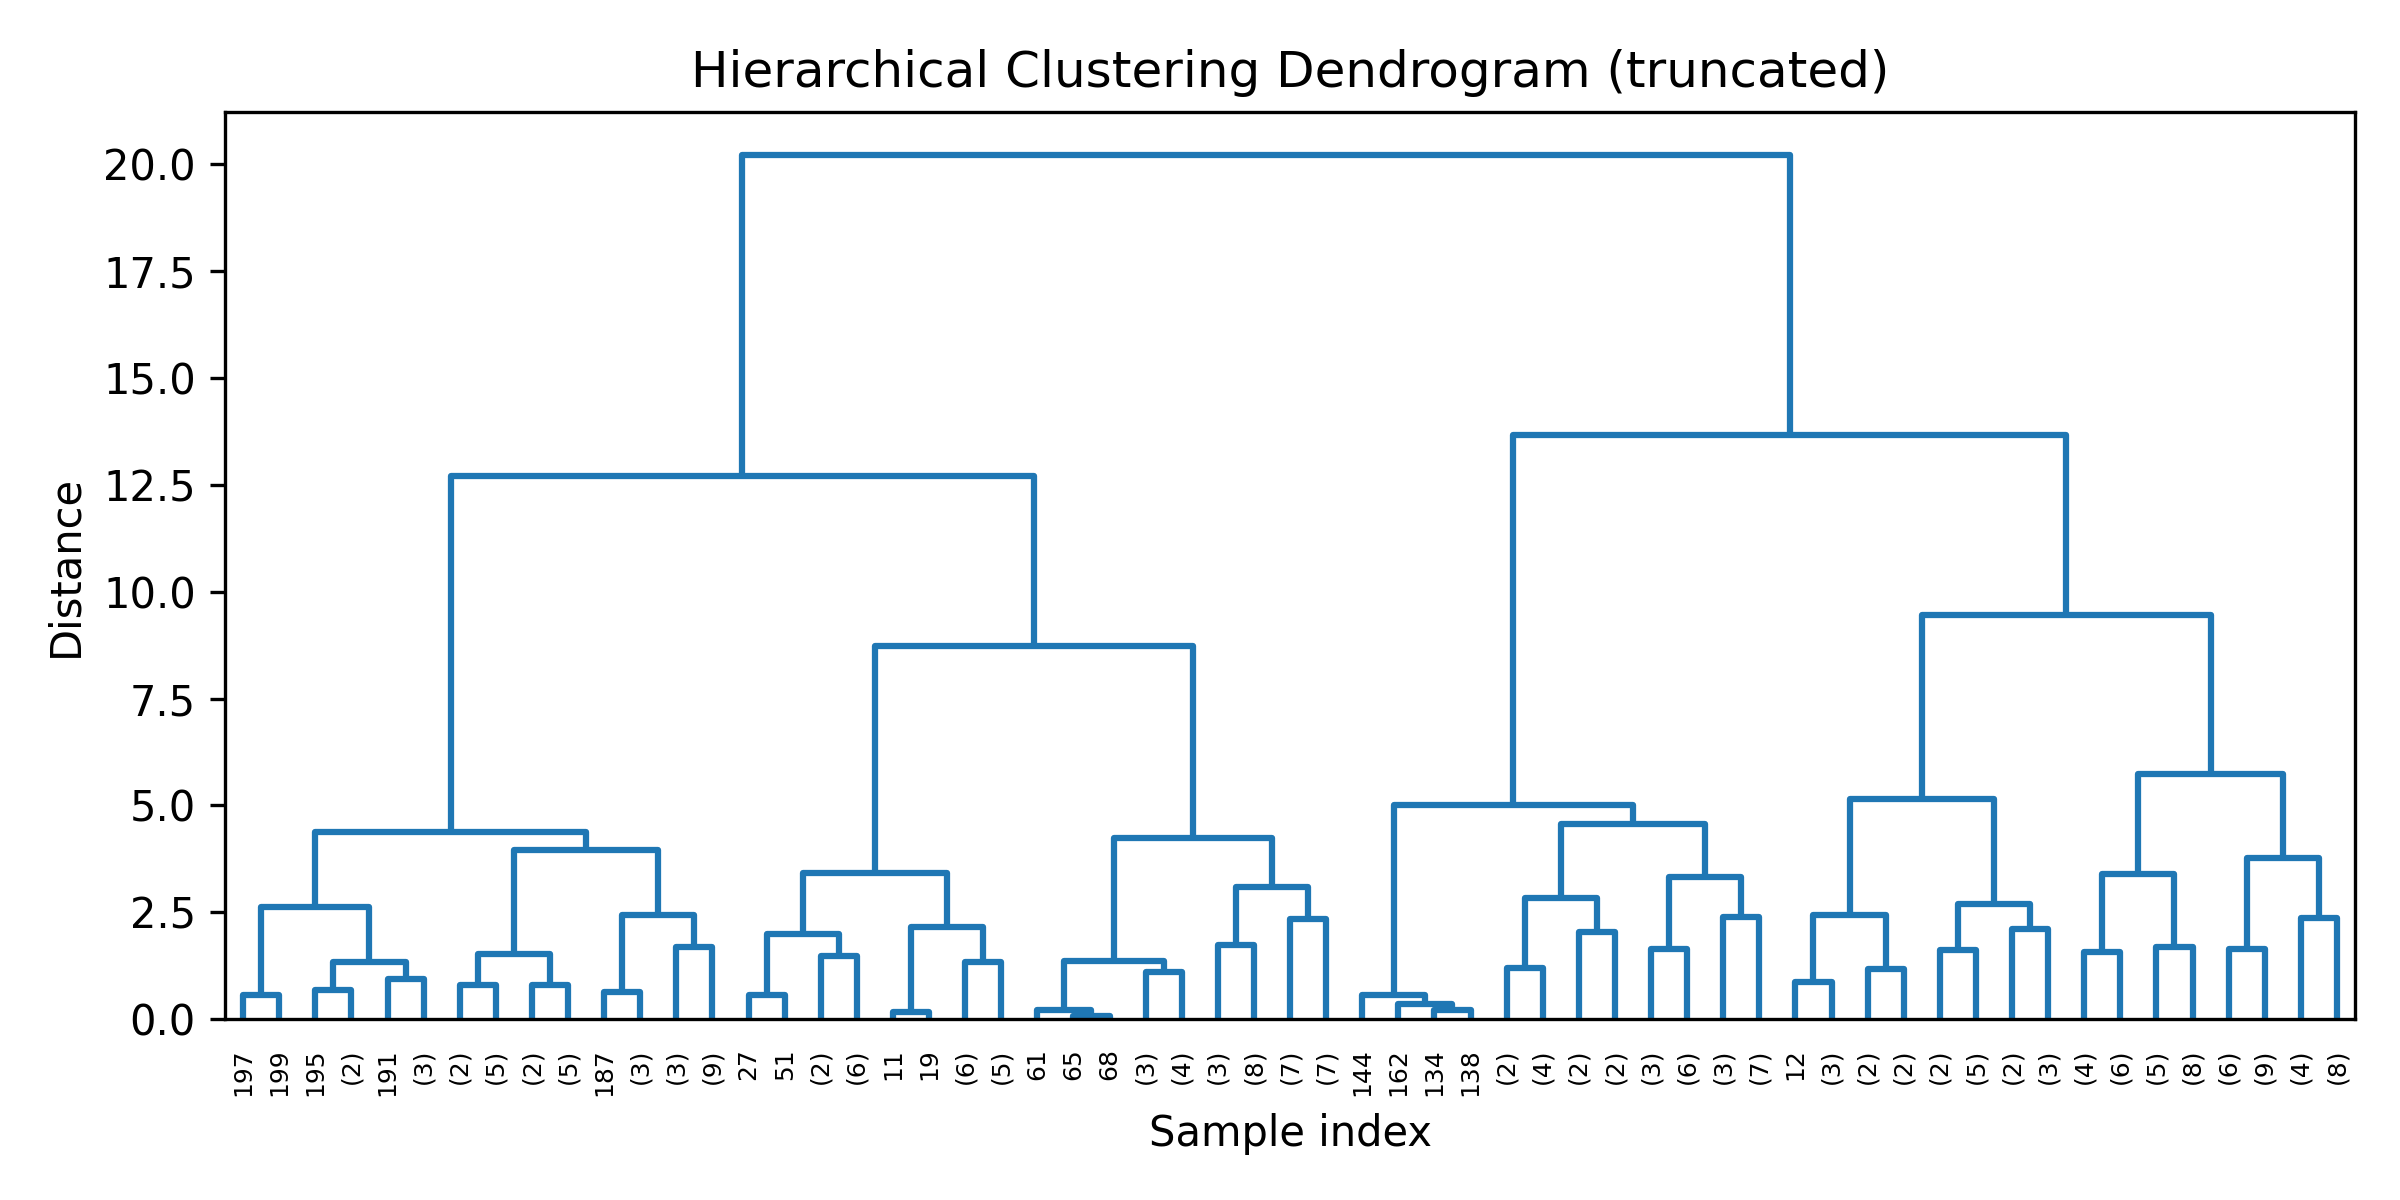
\includegraphics[width=\linewidth]{figures2/dendrogram.png}
    \caption{层次聚类的截断树状图(Ward linkage, level = 5)}
    \label{fig:dendro}
\end{figure}

\paragraph{4.3 代码与文件结构}
\begin{itemize}
    \item 项目根目录包含 \texttt{task1.py} 与 \texttt{task2.py} 两个脚本,分别对应监督与无监督实验。
    \item 生成的图片自动保存于
          \texttt{./figures}(监督学习)与
          \texttt{./figures2}(无监督学习)文件夹,已在 \texttt{task\#.py} 启动时通过 \verb|Path.mkdir| 自动创建。
    \item LaTeX 文档与 \texttt{report.tex} 位于 \texttt{LAB2/} 根目录,编译后生成 \texttt{report.pdf},所有图片通过相对路径引用,确保可重现性。
\end{itemize}

% ---------------- 实验总结 ----------------


\section*{实验总结}

本实验依次完成了监督学习与无监督学习两大任务,系统地验证了缺失值处理策略和聚类方法对模型性能的影响。

\paragraph{监督学习成果} 
基于 Iris 数据集比较了四种缺失值策略与四类经典分类器的组合。结果表明:
\begin{itemize}
    \item \emph{median} 填补在总体准确率(\num{93.3}\%)与加权 $F_1$ 指标上均略优于其他策略
    \item \textbf{Decision Tree}、\textbf{SVM} 与 \textbf{KNN} 在 median 策略下表现最为稳定
    \item \emph{drop} 策略虽然可保持样本纯净度,却因训练集规模收缩导致 LogReg 模型性能明显下降
\end{itemize}

\paragraph{无监督学习成果}
针对 Mall Customers 数据集完成了标准化、降维、肘部法则与轮廓系数分析,得到以下结论:
\begin{itemize}
    \item 通过轮廓系数分析确定最佳簇数 $k=6$
    \item \textbf{K-Means} 取得最佳内部评估指标:Silhouette = \num{0.356},CH = \num{99.7},DB = \num{1.005}
    \item 经验证,K-Means 在该数据集上的聚类效果优于层次聚类与 DBSCAN
\end{itemize}

\paragraph{综合结论}
通过本实验,我们验证了适当的缺失值填补策略(尤其是 median 方法)与合理的簇数选择(基于 Silhouette 系数最大化)能显著提高模型的泛化能力与聚类一致性。这些发现为后续更复杂的数据挖掘任务与模型扩展提供了可靠的技术基准和方法参考。

\end{document}